% Options for packages loaded elsewhere
\PassOptionsToPackage{unicode}{hyperref}
\PassOptionsToPackage{hyphens}{url}
%
\documentclass[
]{article}
\usepackage{lmodern}
\usepackage{amssymb,amsmath}
\usepackage{ifxetex,ifluatex}
\ifnum 0\ifxetex 1\fi\ifluatex 1\fi=0 % if pdftex
  \usepackage[T1]{fontenc}
  \usepackage[utf8]{inputenc}
  \usepackage{textcomp} % provide euro and other symbols
\else % if luatex or xetex
  \usepackage{unicode-math}
  \defaultfontfeatures{Scale=MatchLowercase}
  \defaultfontfeatures[\rmfamily]{Ligatures=TeX,Scale=1}
\fi
% Use upquote if available, for straight quotes in verbatim environments
\IfFileExists{upquote.sty}{\usepackage{upquote}}{}
\IfFileExists{microtype.sty}{% use microtype if available
  \usepackage[]{microtype}
  \UseMicrotypeSet[protrusion]{basicmath} % disable protrusion for tt fonts
}{}
\makeatletter
\@ifundefined{KOMAClassName}{% if non-KOMA class
  \IfFileExists{parskip.sty}{%
    \usepackage{parskip}
  }{% else
    \setlength{\parindent}{0pt}
    \setlength{\parskip}{6pt plus 2pt minus 1pt}}
}{% if KOMA class
  \KOMAoptions{parskip=half}}
\makeatother
\usepackage{xcolor}
\IfFileExists{xurl.sty}{\usepackage{xurl}}{} % add URL line breaks if available
\IfFileExists{bookmark.sty}{\usepackage{bookmark}}{\usepackage{hyperref}}
\hypersetup{
  pdftitle={Ionotropic receptors as the driving force behind human synapse establishment},
  pdfauthor={Lucas H. Viscardi; Danilo O. Imparato; Maria Cátira Bortolini; Rodrigo J. S. Dalmolin},
  pdfkeywords={Evolution, Nervous system},
  hidelinks,
  pdfcreator={LaTeX via pandoc}}
\urlstyle{same} % disable monospaced font for URLs
\usepackage[margin=1in]{geometry}
\usepackage{color}
\usepackage{fancyvrb}
\newcommand{\VerbBar}{|}
\newcommand{\VERB}{\Verb[commandchars=\\\{\}]}
\DefineVerbatimEnvironment{Highlighting}{Verbatim}{commandchars=\\\{\}}
% Add ',fontsize=\small' for more characters per line
\usepackage{framed}
\definecolor{shadecolor}{RGB}{48,48,48}
\newenvironment{Shaded}{\begin{snugshade}}{\end{snugshade}}
\newcommand{\AlertTok}[1]{\textcolor[rgb]{1.00,0.81,0.69}{#1}}
\newcommand{\AnnotationTok}[1]{\textcolor[rgb]{0.50,0.62,0.50}{\textbf{#1}}}
\newcommand{\AttributeTok}[1]{\textcolor[rgb]{0.80,0.80,0.80}{#1}}
\newcommand{\BaseNTok}[1]{\textcolor[rgb]{0.86,0.64,0.64}{#1}}
\newcommand{\BuiltInTok}[1]{\textcolor[rgb]{0.80,0.80,0.80}{#1}}
\newcommand{\CharTok}[1]{\textcolor[rgb]{0.86,0.64,0.64}{#1}}
\newcommand{\CommentTok}[1]{\textcolor[rgb]{0.50,0.62,0.50}{#1}}
\newcommand{\CommentVarTok}[1]{\textcolor[rgb]{0.50,0.62,0.50}{\textbf{#1}}}
\newcommand{\ConstantTok}[1]{\textcolor[rgb]{0.86,0.64,0.64}{\textbf{#1}}}
\newcommand{\ControlFlowTok}[1]{\textcolor[rgb]{0.94,0.87,0.69}{#1}}
\newcommand{\DataTypeTok}[1]{\textcolor[rgb]{0.87,0.87,0.75}{#1}}
\newcommand{\DecValTok}[1]{\textcolor[rgb]{0.86,0.86,0.80}{#1}}
\newcommand{\DocumentationTok}[1]{\textcolor[rgb]{0.50,0.62,0.50}{#1}}
\newcommand{\ErrorTok}[1]{\textcolor[rgb]{0.76,0.75,0.62}{#1}}
\newcommand{\ExtensionTok}[1]{\textcolor[rgb]{0.80,0.80,0.80}{#1}}
\newcommand{\FloatTok}[1]{\textcolor[rgb]{0.75,0.75,0.82}{#1}}
\newcommand{\FunctionTok}[1]{\textcolor[rgb]{0.94,0.94,0.56}{#1}}
\newcommand{\ImportTok}[1]{\textcolor[rgb]{0.80,0.80,0.80}{#1}}
\newcommand{\InformationTok}[1]{\textcolor[rgb]{0.50,0.62,0.50}{\textbf{#1}}}
\newcommand{\KeywordTok}[1]{\textcolor[rgb]{0.94,0.87,0.69}{#1}}
\newcommand{\NormalTok}[1]{\textcolor[rgb]{0.80,0.80,0.80}{#1}}
\newcommand{\OperatorTok}[1]{\textcolor[rgb]{0.94,0.94,0.82}{#1}}
\newcommand{\OtherTok}[1]{\textcolor[rgb]{0.94,0.94,0.56}{#1}}
\newcommand{\PreprocessorTok}[1]{\textcolor[rgb]{1.00,0.81,0.69}{\textbf{#1}}}
\newcommand{\RegionMarkerTok}[1]{\textcolor[rgb]{0.80,0.80,0.80}{#1}}
\newcommand{\SpecialCharTok}[1]{\textcolor[rgb]{0.86,0.64,0.64}{#1}}
\newcommand{\SpecialStringTok}[1]{\textcolor[rgb]{0.80,0.58,0.58}{#1}}
\newcommand{\StringTok}[1]{\textcolor[rgb]{0.80,0.58,0.58}{#1}}
\newcommand{\VariableTok}[1]{\textcolor[rgb]{0.80,0.80,0.80}{#1}}
\newcommand{\VerbatimStringTok}[1]{\textcolor[rgb]{0.80,0.58,0.58}{#1}}
\newcommand{\WarningTok}[1]{\textcolor[rgb]{0.50,0.62,0.50}{\textbf{#1}}}
\usepackage{graphicx,grffile}
\makeatletter
\def\maxwidth{\ifdim\Gin@nat@width>\linewidth\linewidth\else\Gin@nat@width\fi}
\def\maxheight{\ifdim\Gin@nat@height>\textheight\textheight\else\Gin@nat@height\fi}
\makeatother
% Scale images if necessary, so that they will not overflow the page
% margins by default, and it is still possible to overwrite the defaults
% using explicit options in \includegraphics[width, height, ...]{}
\setkeys{Gin}{width=\maxwidth,height=\maxheight,keepaspectratio}
% Set default figure placement to htbp
\makeatletter
\def\fps@figure{htbp}
\makeatother
\setlength{\emergencystretch}{3em} % prevent overfull lines
\providecommand{\tightlist}{%
  \setlength{\itemsep}{0pt}\setlength{\parskip}{0pt}}
\setcounter{secnumdepth}{-\maxdimen} % remove section numbering
\usepackage{booktabs}
\usepackage{longtable}
\usepackage{array}
\usepackage{multirow}
\usepackage{wrapfig}
\usepackage{float}
\usepackage{colortbl}
\usepackage{pdflscape}
\usepackage{tabu}
\usepackage{threeparttable}
\usepackage{threeparttablex}
\usepackage[normalem]{ulem}
\usepackage{makecell}
\usepackage{xcolor}
\usepackage{subfig}
\let\oldShaded\Shaded
\let\endoldShaded\endShaded
\renewenvironment{Shaded}{\scriptsize\oldShaded}{\endoldShaded}
\let\oldverbatim\verbatim
\let\endoldverbatim\endverbatim
\renewenvironment{verbatim}{\scriptsize\oldverbatim}{\endoldverbatim}
\usepackage{caption}
\captionsetup{justification=raggedright,singlelinecheck=false}
\captionsetup{margin={2pt,0pt}}
\floatplacement{figure}{H}

\title{Ionotropic receptors as the driving force behind human synapse
establishment}
\usepackage{etoolbox}
\makeatletter
\providecommand{\subtitle}[1]{% add subtitle to \maketitle
  \apptocmd{\@title}{\par {\large #1 \par}}{}{}
}
\makeatother
\subtitle{Supplementary Material}
\author{Lucas H. Viscardi \and Danilo O. Imparato \and Maria Cátira Bortolini \and Rodrigo J. S. Dalmolin}
\date{}

\begin{document}
\maketitle
\begin{abstract}
The origin of nervous systems is a main theme in biology and its
mechanisms are largely underlied by synaptic neurotransmission. The
search for pan-neuronal genes has failed to explain synapses emergence
since synaptic elements are present in multiple aneural organisms. We
questioned how the interactions among these elements evolved and to what
extent does it relate to our understanding of the nervous systems
complexity. We infer the human neurotransmission gene network based on
genes present in GABAergic, glutamatergic, serotonergic, dopaminergic,
and cholinergic systems, and reconstruct the evolutionary scenario of
synapse emergence. Our results outline the distribution of
neurotransmitter systems and synaptic functions as taxa diverge. We find
that the ionotropic receptors emergence in the cnidarian last common
ancestor was the driving force behind the advent of the anatomical
synapse and the development of nervous systems. We suggest that after
Placozoa origin there was a positive selection under a more restricted
and specific activation of ionotropic receptors. This different
selective pressure counterparting the broader amino acid activation in
plants could be striking for the evolution of the nervous system.
\end{abstract}

{
\setcounter{tocdepth}{3}
\tableofcontents
}
\hypertarget{project-structure}{%
\section{Project structure}\label{project-structure}}

This is the title page

\hypertarget{preprocessing}{%
\section{Preprocessing}\label{preprocessing}}

This topic refers mainly to data wrangling done before the actual
analysis with the intent of making it simpler.

\hypertarget{eukaryota-species-tree}{%
\subsection{Eukaryota species tree}\label{eukaryota-species-tree}}

We opted to use the TimeTree database in order to obtain an standardized
Eukaryota species tree. However, some species were not present in it, so
we devised a way to fill them in based on NCBI Taxonomy data.

\hypertarget{ncbi-taxonomy-tree}{%
\subsubsection{NCBI Taxonomy tree}\label{ncbi-taxonomy-tree}}

First we preprocess NCBI Taxonomy data to leave only STRING eukaryotes,
thus making the task easier. \textbf{Resources}

\begin{table}[H]

\caption{\label{tab:string_species}Lists all organisms in STRING v11.}
\begin{tabular}[t]{rllll>{\raggedright\arraybackslash}p{18em}}
\toprule
\multicolumn{6}{c}{\bgroup\fontsize{12}{14}\selectfont \cellcolor[HTML]{EEEEEE}{\ttfamily{\textbf{string\_species}}}\egroup{}} \\
\cmidrule(l{3pt}r{3pt}){1-6}
\# & Col. name & Col. type & Used? & Example & Description\\
\midrule
\rowcolor{gray!6}  1 & taxid & character & yes & 9606 & NCBI Taxonomy identifier\\
2 & string\_type & character & no & core & if the genome of this species is core or periphery\\
\rowcolor{gray!6}  3 & string\_name & character & yes & Homo sapiens & STRING species name\\
4 & ncbi\_official\_name & character & no & Homo sapiens & NCBI Taxonomy species name\\
\bottomrule
\multicolumn{6}{l}{\textbf{Location: } data-raw/download/species.v11.0.txt}\\
\multicolumn{6}{l}{\textbf{Source: } stringdb-static.org/download/species.v11.0.txt}\\
\end{tabular}
\end{table}
\begin{table}[H]

\caption{\label{tab:ncbi_merged_ids}Links outdated taxon IDs to corresponding new ones.}
\begin{tabular}[t]{rllll>{\raggedright\arraybackslash}p{18em}}
\toprule
\multicolumn{6}{c}{\bgroup\fontsize{12}{14}\selectfont \cellcolor[HTML]{EEEEEE}{\ttfamily{\textbf{ncbi\_merged\_ids}}}\egroup{}} \\
\cmidrule(l{3pt}r{3pt}){1-6}
\# & Col. name & Col. type & Used? & Example & Description\\
\midrule
\rowcolor{gray!6}  1 & taxid & character & yes & 140100 & id of node that has been merged\\
2 & new\_taxid & character & yes & 666 & id of node that is the result of merging\\
\bottomrule
\multicolumn{6}{l}{\textbf{Location: } data-raw/download/taxdump/merged.dmp}\\
\multicolumn{6}{l}{\textbf{Source: } ftp.ncbi.nlm.nih.gov/pub/taxonomy/taxdump.tar.gz}\\
\end{tabular}
\end{table}
\begin{table}[H]

\caption{\label{tab:ncbi_edgelist}Represents taxonomy nodes.}
\begin{tabular}[t]{rllll>{\raggedright\arraybackslash}p{18em}}
\toprule
\multicolumn{6}{c}{\bgroup\fontsize{12}{14}\selectfont \cellcolor[HTML]{EEEEEE}{\ttfamily{\textbf{ncbi\_edgelist}}}\egroup{}} \\
\cmidrule(l{3pt}r{3pt}){1-6}
\# & Col. name & Col. type & Used? & Example & Description\\
\midrule
\rowcolor{gray!6}  1 & taxid & character & yes & 2 & node id in NCBI taxonomy database\\
2 & parent\_taxid & character & yes & 131567 & parent node id in NCBI taxonomy database\\
\rowcolor{gray!6}  3 & rank & character & no & superkingdom & rank of this node\\
4 & ... & ... & no & ... & (too many unrelated fields)\\
\bottomrule
\multicolumn{6}{l}{\textbf{Location: } data-raw/download/taxdump/nodes.dmp}\\
\multicolumn{6}{l}{\textbf{Source: } ftp.ncbi.nlm.nih.gov/pub/taxonomy/taxdump.tar.gz}\\
\end{tabular}
\end{table}
\begin{table}[H]

\caption{\label{tab:ncbi_taxon_names}Links taxon IDs to actual species names.}
\begin{tabular}[t]{rllll>{\raggedright\arraybackslash}p{18em}}
\toprule
\multicolumn{6}{c}{\bgroup\fontsize{12}{14}\selectfont \cellcolor[HTML]{EEEEEE}{\ttfamily{\textbf{ncbi\_taxon\_names}}}\egroup{}} \\
\cmidrule(l{3pt}r{3pt}){1-6}
\# & Col. name & Col. type & Used? & Example & Description\\
\midrule
\rowcolor{gray!6}  1 & taxid & character & yes & 2 & the id of node associated with this name\\
2 & name & character & yes & Monera & name itself\\
\rowcolor{gray!6}  3 & unique\_name & character & no & Monera <bacteria> & the unique variant of this name if name not unique\\
4 & name\_class & character & yes & scientific name & type of name\\
\bottomrule
\multicolumn{6}{l}{\textbf{Location: } data-raw/download/taxdump/names.dmp}\\
\multicolumn{6}{l}{\textbf{Source: } ftp.ncbi.nlm.nih.gov/pub/taxonomy/taxdump.tar.gz}\\
\end{tabular}
\end{table}

\textbf{Duplicated genera}\\
Some species from different kingdoms may have the same genus name.
Duplicated genera must be noted down because we will use them to fill in
missing species at a later time.

\begin{Shaded}
\begin{Highlighting}[]
\CommentTok{# keeping genera nodes}
\NormalTok{genera_taxids <-}\StringTok{ }\NormalTok{ncbi_edgelist }\OperatorTok
\StringTok{  }\KeywordTok{filter}\NormalTok{(rank }\OperatorTok{==}\StringTok{ "genus"}\NormalTok{) }\OperatorTok
\StringTok{  }\KeywordTok{select}\NormalTok{(}\DataTypeTok{taxid =}\NormalTok{ n1, rank)}

\NormalTok{duplicated_genera <-}\StringTok{ }\NormalTok{ncbi_taxon_names }\OperatorTok
\StringTok{  }\CommentTok{# keeping scientific names}
\StringTok{  }\KeywordTok{filter}\NormalTok{(type }\OperatorTok{==}\StringTok{ "scientific name"}\NormalTok{) }\OperatorTok
\StringTok{  }\KeywordTok{select}\NormalTok{(}\DataTypeTok{taxid =}\NormalTok{ name, ncbi_name) }\OperatorTok
\StringTok{  }\KeywordTok{inner_join}\NormalTok{(genera_taxids) }\OperatorTok
\StringTok{  }\CommentTok{# extracting and saving duplicated values}
\StringTok{  }\KeywordTok{pull}\NormalTok{(ncbi_name) }\OperatorTok
\StringTok{  }\KeywordTok{extract}\NormalTok{(}\KeywordTok{duplicated}\NormalTok{(.)) }\OperatorTok
\StringTok{  }\KeywordTok{write}\NormalTok{(}\StringTok{"duplicated_genera.txt"}\NormalTok{)}
\end{Highlighting}
\end{Shaded}

\textbf{Updating STRING taxon IDs}\\
Some organisms taxon IDs are outdated in STRING. We must update them to
work with the most recent NCBI Taxonomy data.

\begin{Shaded}
\begin{Highlighting}[]
\NormalTok{string_species }\OperatorTok
\StringTok{  }\KeywordTok{left_join}\NormalTok{(ncbi_merged_ids) }\OperatorTok
\StringTok{  }\KeywordTok{mutate}\NormalTok{(}\DataTypeTok{new_taxid =} \KeywordTok{coalesce}\NormalTok{(new_taxid, taxid))}
\end{Highlighting}
\end{Shaded}

\textbf{Creating tree graph}\\
The first step is to create a directed graph representing the NCBI
Taxonomy tree.

\begin{Shaded}
\begin{Highlighting}[]
\CommentTok{# leaving only "scientific name" rows}
\NormalTok{ncbi_taxon_names }\OperatorTok
\StringTok{  }\KeywordTok{filter}\NormalTok{(type }\OperatorTok{==}\StringTok{ "scientific name"}\NormalTok{) }\OperatorTok
\StringTok{  }\KeywordTok{select}\NormalTok{(name, ncbi_name)}

\CommentTok{# finding Eukaryota taxid}
\NormalTok{eukaryota_taxon_id <-}\StringTok{ }\KeywordTok{subset}\NormalTok{(ncbi_taxon_names, ncbi_name }\OperatorTok{==}\StringTok{ "Eukaryota"}\NormalTok{, }\StringTok{"name"}\NormalTok{, }\DataTypeTok{drop =} \OtherTok{TRUE}\NormalTok{)}

\CommentTok{# creating graph}
\NormalTok{g <-}\StringTok{ }\KeywordTok{graph_from_data_frame}\NormalTok{(ncbi_edgelist[,}\DecValTok{2}\OperatorTok{:}\DecValTok{1}\NormalTok{], }\DataTypeTok{directed =} \OtherTok{TRUE}\NormalTok{, }\DataTypeTok{vertices =}\NormalTok{ ncbi_taxon_names)}

\CommentTok{# easing memory}
\KeywordTok{rm}\NormalTok{(ncbi_edgelist, ncbi_merged_ids)}
\end{Highlighting}
\end{Shaded}

\textbf{Traversing the graph}\\
The second step is to traverse the graph from the Eukaryota root node to
STRING species nodes. This automatically drops all non-eukaryotes and
results in a species tree representing only STRING eukaryotes (476).

\begin{Shaded}
\begin{Highlighting}[]
\NormalTok{eukaryote_root <-}\StringTok{ }\KeywordTok{V}\NormalTok{(g)[eukaryota_taxon_id]}
\NormalTok{eukaryote_leaves <-}\StringTok{ }\KeywordTok{V}\NormalTok{(g)[string_species[[}\StringTok{"new_taxid"}\NormalTok{]]]}

\CommentTok{# not_found <- subset(string_species, !new_taxid %in% ncbi_taxon_names$name)}

\NormalTok{eukaryote_paths <-}\StringTok{ }\KeywordTok{shortest_paths}\NormalTok{(g, }\DataTypeTok{from =}\NormalTok{ eukaryote_root, }\DataTypeTok{to =}\NormalTok{ eukaryote_leaves, }\DataTypeTok{mode =} \StringTok{"out"}\NormalTok{)}\OperatorTok{$}\NormalTok{vpath}

\NormalTok{eukaryote_vertices <-}\StringTok{ }\NormalTok{eukaryote_paths }\OperatorTok\StringTok{ }\NormalTok{unlist }\OperatorTok\StringTok{ }\NormalTok{unique}

\NormalTok{eukaryote_tree <-}\StringTok{ }\KeywordTok{induced_subgraph}\NormalTok{(g, eukaryote_vertices, }\DataTypeTok{impl =} \StringTok{"create_from_scratch"}\NormalTok{)}
\end{Highlighting}
\end{Shaded}

\textbf{Saving}\\
Saving \texttt{ncbi\_tree} and \texttt{string\_eukaryotes} for package
use. These data files are documented by the package. We also create a
plain text file \texttt{476\_ncbi\_eukaryotes.txt} containing the
updated names of all 476 STRING eukaryotes. This file will be queried
against the TimeTree website.

\begin{Shaded}
\begin{Highlighting}[]
\NormalTok{ncbi_tree <-}\StringTok{ }\NormalTok{treeio}\OperatorTok{::}\KeywordTok{as.phylo}\NormalTok{(eukaryote_tree)}

\NormalTok{string_eukaryotes <-}\StringTok{ }\NormalTok{string_species }\OperatorTok
\StringTok{  }\KeywordTok{filter}\NormalTok{(new_taxid }\OperatorTok\StringTok{ }\NormalTok{ncbi_tree}\OperatorTok{$}\NormalTok{tip.label) }\OperatorTok
\StringTok{  }\KeywordTok{inner_join}\NormalTok{(ncbi_taxon_names, }\DataTypeTok{by =} \KeywordTok{c}\NormalTok{(}\StringTok{"new_taxid"}\NormalTok{ =}\StringTok{ "name"}\NormalTok{))}

\KeywordTok{write}\NormalTok{(string_eukaryotes[[}\StringTok{"ncbi_name"}\NormalTok{]],}\StringTok{"476_ncbi_eukaryotes.txt"}\NormalTok{)}

\KeywordTok{write.tree}\NormalTok{(ncbi_tree, }\StringTok{"tree_ncbi.nwk"}\NormalTok{)}
\NormalTok{usethis}\OperatorTok{::}\KeywordTok{use_data}\NormalTok{(string_eukaryotes, }\DataTypeTok{overwrite =} \OtherTok{TRUE}\NormalTok{)}
\end{Highlighting}
\end{Shaded}



\hypertarget{duplicated-genera}{%
\subsubsection{Duplicated Genera}\label{duplicated-genera}}

Some species from different kingdoms may share the same genus name.
These genera must be noted down because one of the ways we fill in
missing species is by looking at genera names.
For \texttt{taxid\_rank} and \texttt{ncbi\_taxon\_names} see
\hyperref[tab:ncbi_edgelist]{Table 3} and
\hyperref[tab:ncbi_taxon_names]{Table 4}, respectively.

\begin{Shaded}
\begin{Highlighting}[]
\CommentTok{# keeping genera nodes}
\NormalTok{taxid_rank }\OperatorTok\StringTok{ }\KeywordTok{filter}\NormalTok{(rank }\OperatorTok{==}\StringTok{ "genus"}\NormalTok{)}

\CommentTok{# keeping scientific names}
\NormalTok{ncbi_taxon_names }\OperatorTok
\StringTok{  }\KeywordTok{filter}\NormalTok{(type }\OperatorTok{==}\StringTok{ "scientific name"}\NormalTok{) }\OperatorTok
\StringTok{  }\KeywordTok{select}\NormalTok{(taxid, ncbi_name) }\OperatorTok
\StringTok{  }\KeywordTok{inner_join}\NormalTok{(taxid_rank)}

\CommentTok{# extracting and saving duplicated values}
\NormalTok{duplicated_genera <-}\StringTok{ }\NormalTok{ncbi_taxon_names }\OperatorTok
\StringTok{  }\KeywordTok{pull}\NormalTok{(ncbi_name) }\OperatorTok
\StringTok{  }\KeywordTok{extract}\NormalTok{(}\KeywordTok{duplicated}\NormalTok{(.)) }\OperatorTok
\StringTok{  }\KeywordTok{write}\NormalTok{(}\StringTok{"duplicated_genera.txt"}\NormalTok{)}
\end{Highlighting}
\end{Shaded}



\hypertarget{hybrid-tree}{%
\subsubsection{Hybrid tree}\label{hybrid-tree}}

Once we have both the NCBI eukaryotes tree and the list of duplicated
genera, we can start assembling the complete hybrid tree.
\texttt{}~\\
\textbf{Resources}\\
Besides downloading all TimeTree species data
(\texttt{Eukaryota\_species.nwk}) we also need to manually query the
website for the 476 STRING eukaryotes
(\texttt{476\_ncbi\_eukaryotes.txt}). The file is called
\texttt{476\_ncbi\_eukaryotes.txt} because it contains updated NCBI
Taxonomy names rather than STRING outdated names. This ensures better
results.

\begin{Shaded}
\begin{Highlighting}[]
\KeywordTok{download_if_missing}\NormalTok{(}
  \KeywordTok{paste0}\NormalTok{(}\StringTok{"http://timetree.org/ajax/direct_download"}\NormalTok{,}
         \StringTok{"?direct-download-format=newick"}\NormalTok{,}
         \StringTok{"&direct-download-id=23070"}\NormalTok{,}
         \StringTok{"&direct-download-rank=species"}\NormalTok{),}
  \StringTok{"Eukaryota_species.nwk"}
\NormalTok{)}
\end{Highlighting}
\end{Shaded}

\texttt{timetree\_newick} is the tree obtained by manually uploading
\texttt{476\_ncbi\_eukaryotes.txt} to the TimeTree website.
\texttt{tree\_85k} is the complete Eukaryota tree we have just
downloaded.

\begin{Shaded}
\begin{Highlighting}[]
\CommentTok{# loading species names and taxon ids}
\KeywordTok{load}\NormalTok{(}\StringTok{"../data/string_eukaryotes.rda"}\NormalTok{)}

\CommentTok{# loading newick tree manually obtained from timetree}
\NormalTok{timetree_newick <-}\StringTok{ }\KeywordTok{read.tree}\NormalTok{(}\StringTok{"download/timetree_335_eukaryotes.nwk"}\NormalTok{)}

\CommentTok{# the following genera names are unreliable and should not be searched for}
\NormalTok{duplicated_genera <-}\StringTok{ }\KeywordTok{scan}\NormalTok{(}\StringTok{"duplicated_genera.txt"}\NormalTok{, }\DataTypeTok{what =} \StringTok{"character"}\NormalTok{)}

\CommentTok{# loading all TimeTree species data we have just download (85000 species)}
\NormalTok{tree_85k <-}\StringTok{ }\KeywordTok{read.tree}\NormalTok{(}\StringTok{"download/Eukaryota_species.nwk"}\NormalTok{)}
\end{Highlighting}
\end{Shaded}

\textbf{Unfound species with matching genera}\\
Some of the 476 STRING eukaryotes are not present in the TimeTree
database. However, sometimes TimeTree does contain tree data for closely
related species (e.g.~\emph{Monosiga brevicollis} is not present, but
\emph{Monosiga ovata} is). Therefore, we can use these closely related
species as proxies for the actual species. This is done by searching for
genera names in the complete database (\texttt{Eukaryota\_species.nwk}).
In the given \emph{Monosiga brevicollis} example, we search for
\emph{Monosiga} in the complete database. We see that there is
information for at least one other species of the \emph{Monosiga} genus
(in this case, \emph{Monosiga ovata}), so we add \emph{Monosiga
brevicollis} as a sister branch to the found species.

When you search for a term in TimeTree, it uses a synonym list obtained
from NCBI to try to resolve it. Sometimes TimeTree will resolve a
searched term to a scientific name different from the one you searched
for. The problem with this is that TimeTree does not make it obvious
that it is returning a different term. The first step is to find out
which species resolved to different names in the
\texttt{timetree\_335\_eukaryotes.nwk} file:

\begin{Shaded}
\begin{Highlighting}[]
\CommentTok{# plot(timetree_newick %>% ladderize, type = "cladogram", use.edge.length = F)}

\CommentTok{# replacing timetree species underscores with spaces}
\NormalTok{timetree_newick[[}\StringTok{"tip.label"}\NormalTok{]] }\OperatorTok\StringTok{ }\KeywordTok{str_replace_all}\NormalTok{(}\StringTok{"_"}\NormalTok{, }\StringTok{" "}\NormalTok{)}

\CommentTok{# which timetree species' names exactly match with ncbi's}
\NormalTok{taxid_indexes <-}\StringTok{ }\NormalTok{timetree_newick[[}\StringTok{"tip.label"}\NormalTok{]] }\OperatorTok\StringTok{ }\KeywordTok{match}\NormalTok{(string_eukaryotes[[}\StringTok{"ncbi_name"}\NormalTok{]])}

\CommentTok{# find out which timetree species names didn't exactly match ncbi's}
\NormalTok{unmatched_names <-}\StringTok{ }\NormalTok{timetree_newick[[}\StringTok{"tip.label"}\NormalTok{]] }\OperatorTok\StringTok{ }\NormalTok{magrittr}\OperatorTok{::}\KeywordTok{extract}\NormalTok{(taxid_indexes }\OperatorTok\StringTok{ }\NormalTok{is.na)}
\KeywordTok{print}\NormalTok{(unmatched_names)}
\end{Highlighting}
\end{Shaded}

\begin{verbatim}
## [1] "Cercospora fijiensis"     "Arthroderma benhamiae"   
## [3] "Macropus eugenii"         "Ostreococcus lucimarinus"
## [5] "Oryza nivara"
\end{verbatim}

\begin{Shaded}
\begin{Highlighting}[]
\CommentTok{# manually creating lookup table to be joined}
\NormalTok{ncbi_to_timetree <-}\StringTok{ }\KeywordTok{tribble}\NormalTok{(}
  \OperatorTok{~}\NormalTok{timetree_name,              }\OperatorTok{~}\NormalTok{ncbi_name,}
  \StringTok{"Cercospora fijiensis"}\NormalTok{,      }\StringTok{"Pseudocercospora fijiensis"}\NormalTok{,}
  \StringTok{"Arthroderma benhamiae"}\NormalTok{,     }\StringTok{"Trichophyton benhamiae"}\NormalTok{,}
  \StringTok{"Macropus eugenii"}\NormalTok{,          }\StringTok{"Notamacropus eugenii"}\NormalTok{,}
  \StringTok{"Ostreococcus lucimarinus"}\NormalTok{,  }\StringTok{"Ostreococcus sp. 'lucimarinus'"}\NormalTok{,}
  \StringTok{"Oryza nivara"}\NormalTok{,              }\StringTok{"Oryza sativa f. spontanea"}
\NormalTok{)}

\CommentTok{# joining info}
\NormalTok{species_dictionary <-}\StringTok{ }\NormalTok{string_eukaryotes }\OperatorTok\StringTok{ }\KeywordTok{left_join}\NormalTok{(ncbi_to_timetree)}

\CommentTok{# coalescing NAs to ncbi_name}
\NormalTok{species_dictionary }\OperatorTok
\StringTok{  }\KeywordTok{mutate}\NormalTok{(}\DataTypeTok{timetree_name =} \KeywordTok{coalesce}\NormalTok{(timetree_name, ncbi_name)) }\OperatorTok
\StringTok{  }\KeywordTok{mutate}\NormalTok{(}\DataTypeTok{timetree_name =} \KeywordTok{ifelse}\NormalTok{(timetree_name }\OperatorTok\StringTok{ }\NormalTok{timetree_newick[[}\StringTok{"tip.label"}\NormalTok{]], timetree_name, }\OtherTok{NA}\NormalTok{))}
\end{Highlighting}
\end{Shaded}

Now we can start looking for unfound species genera in the complete tree
data.

\begin{Shaded}
\begin{Highlighting}[]
\CommentTok{# annotating genera}
\NormalTok{species_dictionary }\OperatorTok
\StringTok{  }\KeywordTok{mutate}\NormalTok{(}\DataTypeTok{genus_search =} \KeywordTok{coalesce}\NormalTok{(timetree_name, ncbi_name) }\OperatorTok
\StringTok{  }\KeywordTok{strsplit}\NormalTok{(}\StringTok{" "}\NormalTok{) }\OperatorTok
\StringTok{  }\KeywordTok{sapply}\NormalTok{(}\StringTok{"["}\NormalTok{, }\DecValTok{1}\NormalTok{))}

\CommentTok{# unique genera}
\NormalTok{selected_genera <-}\StringTok{ }\NormalTok{species_dictionary[[}\StringTok{"genus_search"}\NormalTok{]] }\OperatorTok\StringTok{ }\NormalTok{unique}

\CommentTok{# these are unreliable selected_genera:}
\NormalTok{unreliable_genera <-}\StringTok{ }\KeywordTok{intersect}\NormalTok{(selected_genera, duplicated_genera)}

\CommentTok{# ensuring a cleaner newick file with only necessary data}
\CommentTok{# this is actually really important}
\NormalTok{tree_85k[[}\StringTok{"node.label"}\NormalTok{]] <-}\StringTok{ }\OtherTok{NULL}
\NormalTok{tree_85k[[}\StringTok{"edge.length"}\NormalTok{]] <-}\StringTok{ }\OtherTok{NULL}

\CommentTok{# replacing timetree's underscores with spaces}
\NormalTok{tree_85k[[}\StringTok{"tip.label"}\NormalTok{]] }\OperatorTok\StringTok{ }\KeywordTok{str_replace_all}\NormalTok{(}\StringTok{"_"}\NormalTok{, }\StringTok{" "}\NormalTok{)}

\CommentTok{# storing genus}
\NormalTok{tree_85k[[}\StringTok{"tip.genus"}\NormalTok{]] <-}\StringTok{ }\KeywordTok{sapply}\NormalTok{(}\KeywordTok{strsplit}\NormalTok{(tree_85k[[}\StringTok{"tip.label"}\NormalTok{]],}\StringTok{" "}\NormalTok{), }\StringTok{"["}\NormalTok{, }\DecValTok{1}\NormalTok{)}
\NormalTok{tree_85k_genera <-}\StringTok{ }\NormalTok{tree_85k[[}\StringTok{"tip.genus"}\NormalTok{]] }\OperatorTok\StringTok{ }\NormalTok{unique}

\CommentTok{# subtracting unreliable genera}
\NormalTok{tree_85k_genera }\OperatorTok\StringTok{ }\KeywordTok{setdiff}\NormalTok{(unreliable_genera)}

\CommentTok{# keeping only selected genera, including unreliable ones}
\NormalTok{tree_genus <-}\StringTok{ }\NormalTok{tree_85k }\OperatorTok\StringTok{ }\KeywordTok{keep.tip}\NormalTok{(., tip.label[tip.genus }\OperatorTok\StringTok{ }\NormalTok{selected_genera])}
\NormalTok{tree_genus[[}\StringTok{"tip.genus"}\NormalTok{]] <-}\StringTok{ }\KeywordTok{sapply}\NormalTok{(}\KeywordTok{strsplit}\NormalTok{(tree_genus[[}\StringTok{"tip.label"}\NormalTok{]],}\StringTok{" "}\NormalTok{), }\StringTok{"["}\NormalTok{, }\DecValTok{1}\NormalTok{)}

\CommentTok{# unfound species which genera are present in the 85k tree}
\NormalTok{unfound_species <-}\StringTok{ }\NormalTok{species_dictionary }\OperatorTok
\StringTok{  }\KeywordTok{filter}\NormalTok{(}\KeywordTok{is.na}\NormalTok{(timetree_name) }\OperatorTok{&}\StringTok{ }\NormalTok{genus_search }\OperatorTok\StringTok{ }\NormalTok{tree_85k_genera)}
\end{Highlighting}
\end{Shaded}

Once we figured out which species have proxy genera in the complete
data, we can start filling them in as sister branches.

\begin{Shaded}
\begin{Highlighting}[]
\CommentTok{# for each unfound species which genus is present in the 85k tree,}
\ControlFlowTok{for}\NormalTok{(i }\ControlFlowTok{in} \DecValTok{1}\OperatorTok{:}\KeywordTok{nrow}\NormalTok{(unfound_species))\{}
  \CommentTok{# we search for all species of this genus ("sister species") in the 85k tree}
  \CommentTok{# this part is tricky because bind.tip rebuilds the tree from scratch}
  \CommentTok{# so we need to keep removing underscores. there are better ways to do this.}
\NormalTok{  tip_genus <-}\StringTok{ }\NormalTok{tree_genus[[}\StringTok{"tip.label"}\NormalTok{]] }\OperatorTok\StringTok{ }\KeywordTok{strsplit}\NormalTok{(}\StringTok{"[_ ]"}\NormalTok{) }\OperatorTok\StringTok{ }\KeywordTok{sapply}\NormalTok{(}\StringTok{"["}\NormalTok{, }\DecValTok{1}\NormalTok{)}
\NormalTok{  sister_species <-}\StringTok{ }\NormalTok{tree_genus[[}\StringTok{"tip.label"}\NormalTok{]][tip_genus }\OperatorTok{==}\StringTok{ }\NormalTok{unfound_species[[i, }\StringTok{"genus_search"}\NormalTok{]]]}
  \CommentTok{# we obtain the sister_species' most recent common ancestor (MRCA)}
  \CommentTok{# c(.[1]) is a hack because the MRCA function only works with at least 2 nodes}
\NormalTok{  where <-}\StringTok{ }\KeywordTok{getMRCA}\NormalTok{(tree_genus, sister_species }\OperatorTok\StringTok{ }\KeywordTok{c}\NormalTok{(.[}\DecValTok{1}\NormalTok{]))}
  \CommentTok{# and then add a leaf node linked to this MRCA}
\NormalTok{  tree_genus }\OperatorTok\StringTok{ }\KeywordTok{bind.tip}\NormalTok{(}\DataTypeTok{tip.label =}\NormalTok{ unfound_species[[i, }\StringTok{"ncbi_name"}\NormalTok{]], }\DataTypeTok{where =}\NormalTok{ where)}
\NormalTok{\}}

\CommentTok{# for some reason bind.tip adds underscores to species names}
\NormalTok{tree_genus[[}\StringTok{"tip.label"}\NormalTok{]] }\OperatorTok\StringTok{ }\KeywordTok{str_replace_all}\NormalTok{(}\StringTok{"_"}\NormalTok{, }\StringTok{" "}\NormalTok{)}

\CommentTok{# keeping track of found species}
\NormalTok{found_species <-}\StringTok{ }\NormalTok{species_dictionary }\OperatorTok\StringTok{ }\KeywordTok{filter}\NormalTok{(}\OperatorTok{!}\KeywordTok{is.na}\NormalTok{(timetree_name) }\OperatorTok{|}\StringTok{ }\NormalTok{genus_search }\OperatorTok\StringTok{ }\NormalTok{tree_85k_genera)}
\CommentTok{# forced_name means it either was found in timetree or we forced it by looking at genera names}
\NormalTok{found_species }\OperatorTok\StringTok{ }\KeywordTok{mutate}\NormalTok{(}\DataTypeTok{forced_name =} \KeywordTok{coalesce}\NormalTok{(timetree_name, ncbi_name))}

\CommentTok{# so we keep only found species in this tree we are building (timetree + forced by genera)}
\NormalTok{tree_genus }\OperatorTok\StringTok{ }\KeywordTok{keep.tip}\NormalTok{(found_species[[}\StringTok{"forced_name"}\NormalTok{]])}

\CommentTok{# which found_species rows correspond to each tip.label?}
\NormalTok{match_tiplabel_name <-}\StringTok{ }\KeywordTok{match}\NormalTok{(tree_genus[[}\StringTok{"tip.label"}\NormalTok{]], found_species[[}\StringTok{"forced_name"}\NormalTok{]])}

\NormalTok{tree_genus }\OperatorTok\StringTok{ }\KeywordTok{list_modify}\NormalTok{(}
\CommentTok{# converting to ncbi taxids}
  \DataTypeTok{tip.label =}\NormalTok{ found_species[[}\StringTok{"new_taxid"}\NormalTok{]][match_tiplabel_name]}
\NormalTok{)}
\end{Highlighting}
\end{Shaded}

\textbf{Species of unfound genera}\\
In this part, we try to fill in the remaining missing species (those
which genera were not found in TimeTree) by searching for their closest
relatives (according to NCBI Taxonomy) that are present in the current
tree. Once we find its two closest relatives, we can add the missing
species as a branch from their LCA. This is a conservative approach.

\begin{Shaded}
\begin{Highlighting}[]
\CommentTok{# converting ncbi phylo to igraph}
\NormalTok{graph_ncbi <-}\StringTok{ }\KeywordTok{read.tree}\NormalTok{(}\StringTok{"tree_ncbi.nwk"}\NormalTok{) }\OperatorTok\StringTok{ }\KeywordTok{as.igraph.phylo}\NormalTok{(}\DataTypeTok{directed =} \OtherTok{TRUE}\NormalTok{)}

\CommentTok{# converting phylo to igraph}
\NormalTok{graph_genus <-}\StringTok{ }\KeywordTok{as.igraph.phylo}\NormalTok{(tree_genus, }\DataTypeTok{directed =} \OtherTok{TRUE}\NormalTok{)}

\CommentTok{# for each species which genus is not in timetree}
\CommentTok{# we'll look for its two closest species (in the NCBI tree) which are present in the tree_genus we just built}
\NormalTok{unfound_genera <-}\StringTok{ }\NormalTok{species_dictionary }\OperatorTok\StringTok{ }\KeywordTok{filter}\NormalTok{(}\KeywordTok{is.na}\NormalTok{(timetree_name) }\OperatorTok{&}\StringTok{ }\OperatorTok{!}\NormalTok{genus_search }\OperatorTok\StringTok{ }\NormalTok{tree_85k_genera)}

\CommentTok{# this is the igraph equivalent of "phylo_tree$tip.label"}
\NormalTok{tip_nodes <-}\StringTok{ }\KeywordTok{V}\NormalTok{(graph_ncbi)[}\KeywordTok{degree}\NormalTok{(graph_ncbi, }\DataTypeTok{mode =} \StringTok{"out"}\NormalTok{) }\OperatorTok{==}\StringTok{ }\DecValTok{0}\NormalTok{]}

\CommentTok{# undirected distances between all species nodes}
\NormalTok{tip_distances <-}\StringTok{ }\NormalTok{graph_ncbi }\OperatorTok
\StringTok{  }\KeywordTok{distances}\NormalTok{(}\DataTypeTok{v =}\NormalTok{ tip_nodes, }\DataTypeTok{to =}\NormalTok{ tip_nodes, }\DataTypeTok{mode =} \StringTok{"all"}\NormalTok{) }\OperatorTok
\StringTok{  }\KeywordTok{as_tibble}\NormalTok{(}\DataTypeTok{rownames =} \StringTok{"from"}\NormalTok{) }\OperatorTok
\StringTok{  }\KeywordTok{pivot_longer}\NormalTok{(}\OperatorTok{-}\NormalTok{from, }\DataTypeTok{names_to =} \StringTok{"to"}\NormalTok{, }\DataTypeTok{values_to =} \StringTok{"distance"}\NormalTok{)}

\CommentTok{# removing self references (zero distances)}
\NormalTok{tip_distances }\OperatorTok\StringTok{ }\KeywordTok{filter}\NormalTok{(distance }\OperatorTok{>}\StringTok{ }\DecValTok{0}\NormalTok{)}

\CommentTok{# we only want to search for species of unfound genera}
\NormalTok{tip_distances }\OperatorTok\StringTok{ }\KeywordTok{inner_join}\NormalTok{(unfound_genera }\OperatorTok\StringTok{ }\KeywordTok{select}\NormalTok{(}\DataTypeTok{from =}\NormalTok{ new_taxid))}

\CommentTok{# we only want to find species already present in the genus_tree}
\NormalTok{tip_distances }\OperatorTok\StringTok{ }\KeywordTok{inner_join}\NormalTok{(found_species }\OperatorTok\StringTok{ }\KeywordTok{select}\NormalTok{(}\DataTypeTok{to =}\NormalTok{ new_taxid))}

\CommentTok{# we only want the two closest relatives}
\NormalTok{tip_distances }\OperatorTok
\StringTok{  }\KeywordTok{group_by}\NormalTok{(from) }\OperatorTok
\StringTok{  }\KeywordTok{top_n}\NormalTok{(}\OperatorTok{-}\DecValTok{2}\NormalTok{, distance) }\OperatorTok\StringTok{ }\CommentTok{# top 2 smallest distances}
\StringTok{  }\KeywordTok{top_n}\NormalTok{(}\DecValTok{2}\NormalTok{, to) }\CommentTok{# more than 2 species have the same smallest distance, so we get the first ones}

\CommentTok{# out distance matrix between all nodes in tree, needed to find MRCAs}
\NormalTok{out_distances <-}\StringTok{ }\NormalTok{graph_genus }\OperatorTok\StringTok{ }\KeywordTok{distances}\NormalTok{(}\DataTypeTok{mode =} \StringTok{"out"}\NormalTok{)}

\CommentTok{# for each species of unfound genera,}
\CommentTok{# we find the MRCA for its two closest relatives}
\NormalTok{unfound_genera_mrca <-}\StringTok{ }\NormalTok{tip_distances }\OperatorTok\StringTok{ }\KeywordTok{group_by}\NormalTok{(from) }\OperatorTok\StringTok{ }\KeywordTok{summarise}\NormalTok{(}\DataTypeTok{mrca =}\NormalTok{ \{}
  \CommentTok{# which rows have no infinite distances? the last one represents the MRCA}
\NormalTok{  mrca_row_index <-}\StringTok{ }\KeywordTok{max}\NormalTok{(}\KeywordTok{which}\NormalTok{(}\KeywordTok{rowSums}\NormalTok{(}\KeywordTok{is.infinite}\NormalTok{(out_distances[, to])) }\OperatorTok{==}\StringTok{ }\DecValTok{0}\NormalTok{))}
  \KeywordTok{rownames}\NormalTok{(out_distances)[mrca_row_index]}
\NormalTok{\})}

\CommentTok{# adding unfound genera species nodes}
\NormalTok{graph_genus }\OperatorTok\StringTok{ }\KeywordTok{add_vertices}\NormalTok{(}\KeywordTok{nrow}\NormalTok{(unfound_genera_mrca), }\DataTypeTok{color =} \StringTok{"red"}\NormalTok{, }\DataTypeTok{attr =} \KeywordTok{list}\NormalTok{(}\DataTypeTok{name =}\NormalTok{ unfound_genera_mrca[[}\StringTok{"from"}\NormalTok{]]))}

\CommentTok{# defining unfound genera species edges}
\CommentTok{# edges_to_add[1] -> edges_to_add[2], edges_to_add[2] -> edges_to_add[3]...}
\NormalTok{edges_to_add <-}\StringTok{ }\KeywordTok{V}\NormalTok{(graph_genus)[unfound_genera_mrca }\OperatorTok\StringTok{ }\KeywordTok{select}\NormalTok{(mrca, from) }\OperatorTok\StringTok{ }\NormalTok{t }\OperatorTok\StringTok{ }\NormalTok{as.vector]}\OperatorTok{$}\NormalTok{name}

\CommentTok{# connecting species leafs to the supposed MRCA}
\NormalTok{graph_genus }\OperatorTok\StringTok{ }\KeywordTok{add_edges}\NormalTok{(}\KeywordTok{V}\NormalTok{(graph_genus)[edges_to_add])}

\CommentTok{# plotting}
\CommentTok{# plot(as.undirected(graph_genus), layout = layout_as_tree(graph_genus), vertex.label = NA, vertex.size=2)}

\CommentTok{# finally converting to phylo format}
\NormalTok{phylo_graph_genus <-}\StringTok{ }\NormalTok{treeio}\OperatorTok{::}\KeywordTok{as.phylo}\NormalTok{(graph_genus)}

\CommentTok{# which species_dictionary rows correspond to each tip.label?}
\NormalTok{match_tiplabel_taxid <-}\StringTok{ }\KeywordTok{match}\NormalTok{(phylo_graph_genus[[}\StringTok{"tip.label"}\NormalTok{]], species_dictionary[[}\StringTok{"new_taxid"}\NormalTok{]])}

\NormalTok{phylo_graph_genus }\OperatorTok\StringTok{ }\KeywordTok{list_modify}\NormalTok{(}
  \CommentTok{# adding tip.alias (this is not exported with write.tree)}
  \DataTypeTok{tip.alias =}\NormalTok{ species_dictionary[[}\StringTok{"string_name"}\NormalTok{]][match_tiplabel_taxid],}
  \CommentTok{# converting back to string ids}
  \DataTypeTok{tip.label =}\NormalTok{ species_dictionary[[}\StringTok{"taxid"}\NormalTok{]][match_tiplabel_taxid]}
\NormalTok{)}

\CommentTok{# ensuring a cleaner newick file with only necessary data}
\NormalTok{phylo_graph_genus[[}\StringTok{"node.label"}\NormalTok{]] <-}\StringTok{ }\OtherTok{NULL}
\NormalTok{phylo_graph_genus[[}\StringTok{"edge.length"}\NormalTok{]] <-}\StringTok{ }\OtherTok{NULL}

\CommentTok{# usethis::use_data(phylo_graph_genus, overwrite = TRUE)}
\CommentTok{# write.tree(phylo_graph_genus, "../data/hybrid_tree.nwk")}
\end{Highlighting}
\end{Shaded}

\textbf{Ctenophora as sister to all animals}\\
According to TimeTree, Ctenophora remains as a sister group to Cnidaria.
We believe the most recent consensus in literature is to consider them a
sister group to all animals. The following code block moves
\emph{Mnemiopsis leidyi}, the only ctenophore in our analysis, to the
base of the metazoan lineage.

\begin{Shaded}
\begin{Highlighting}[]
\CommentTok{# reordering tip.labels}
\NormalTok{from_to <-}\StringTok{ }\KeywordTok{c}\NormalTok{(}
  \StringTok{"400682"}\NormalTok{ =}\StringTok{ "27923"}\NormalTok{,  }\CommentTok{# amphimedon to mnemiopsis}
  \StringTok{"10228"}\NormalTok{  =}\StringTok{ "400682"}\NormalTok{, }\CommentTok{# trichoplax to amphimedon}
  \StringTok{"27923"}\NormalTok{  =}\StringTok{ "10228"}   \CommentTok{# mnemiopsis to trichoplax}
\NormalTok{)}

\NormalTok{modified_phylo <-}\StringTok{ }\NormalTok{phylo_graph_genus}

\NormalTok{modified_phylo[[}\StringTok{"tip.label"}\NormalTok{]] }\OperatorTok\StringTok{ }\KeywordTok{recode}\NormalTok{(}\OperatorTok{!!!}\NormalTok{from_to)}

\KeywordTok{write.tree}\NormalTok{(modified_phylo, }\StringTok{"../data/hybrid_tree_modified.nwk"}\NormalTok{)}
\end{Highlighting}
\end{Shaded}

\begin{figure}
\centering
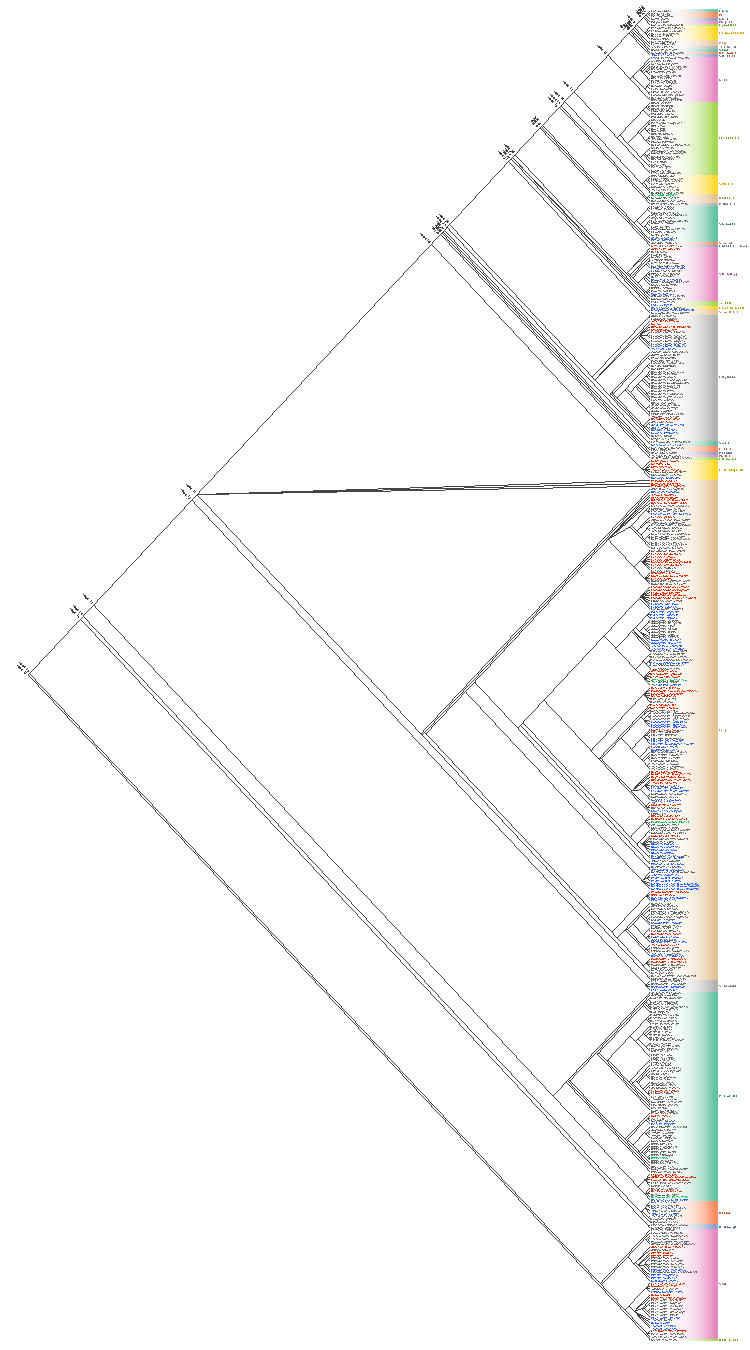
\includegraphics[width=\textwidth,height=0.95\textheight]{../data-raw/tree_hybrid.pdf}
\caption{Complete 476 eukaryotes tree. Green species have been filled in
by a genus proxy in TimeTree. Red species have been filled in by looking
at NCBI Taxonomy. Clade naming is described further in this document.}
\end{figure}


\hypertarget{gene-selection-and-annotation}{%
\subsection{Gene selection and
annotation}\label{gene-selection-and-annotation}}

The anchoring point for this study is basic annotation about genes and
the pathways in which they participate. This section describes the
process of structuring such data. In the end we will have a table to
which all kinds of additional data will be left joined into.
\hypertarget{neurotransmitter-systems-annotation}{%
\subsubsection{Neurotransmitter systems
annotation}\label{neurotransmitter-systems-annotation}}

We start by querying the KEGG api for the pathways of interest.
Resulting data is then pivoted to a wider format.

\begin{table}[H]

\caption{\label{tab:link_pathway_entrez}All links between genes and pathways in KEGG.}
\begin{tabular}[t]{rlllll}
\toprule
\multicolumn{6}{c}{\bgroup\fontsize{12}{14}\selectfont \cellcolor[HTML]{EEEEEE}{\ttfamily{\textbf{link\_pathway\_entrez}}}\egroup{}} \\
\cmidrule(l{3pt}r{3pt}){1-6}
\# & Col. name & Col. type & Used? & Example & Description\\
\midrule
\rowcolor{gray!6}  1 & entrez\_id & character & yes & hsa:10411 & NCBI Taxonomy identifier\\
2 & pathway\_id & character & yes & path:hsa04726 & KEGG pathway ID\\
\bottomrule
\multicolumn{6}{l}{\textbf{Location: } data-raw/download/link\_pathway\_entrez.tsv}\\
\multicolumn{6}{l}{\textbf{Source: } http://rest.kegg.jp/link/pathway/hsa}\\
\end{tabular}
\end{table}

\begin{Shaded}
\begin{Highlighting}[]
\NormalTok{pathways <-}\StringTok{ }\KeywordTok{tribble}\NormalTok{(}
  \OperatorTok{~}\NormalTok{pathway_id,      }\OperatorTok{~}\NormalTok{pathway_name, }
  \StringTok{"path:hsa04724"}\NormalTok{,  }\StringTok{"glutamatergic"}\NormalTok{,}
  \StringTok{"path:hsa04725"}\NormalTok{,  }\StringTok{"cholinergic"}\NormalTok{,  }
  \StringTok{"path:hsa04726"}\NormalTok{,  }\StringTok{"serotonergic"}\NormalTok{, }
  \StringTok{"path:hsa04727"}\NormalTok{,  }\StringTok{"gabaergic"}\NormalTok{,    }
  \StringTok{"path:hsa04728"}\NormalTok{,  }\StringTok{"dopaminergic"}
\NormalTok{)}

\CommentTok{# removing hsa prefix}
\NormalTok{link_pathway_entrez[[}\StringTok{"entrez_id"}\NormalTok{]] }\OperatorTok\StringTok{ }\KeywordTok{str_split_n}\NormalTok{(}\StringTok{":"}\NormalTok{, }\DecValTok{2}\NormalTok{)}

\CommentTok{# filtering for pathways of interest and pivoting}
\NormalTok{gene_pathways <-}\StringTok{ }\KeywordTok{inner_join}\NormalTok{(link_pathway_entrez, pathways) }\OperatorTok
\StringTok{  }\KeywordTok{mutate}\NormalTok{(}\DataTypeTok{n =} \DecValTok{1}\NormalTok{) }\OperatorTok
\StringTok{  }\KeywordTok{pivot_wider}\NormalTok{(}
    \DataTypeTok{id_cols     =}\NormalTok{ entrez_id,}
    \DataTypeTok{names_from  =}\NormalTok{ pathway_name, }
    \DataTypeTok{values_from =}\NormalTok{ n,}
    \DataTypeTok{values_fn   =} \KeywordTok{list}\NormalTok{(}\DataTypeTok{n =}\NormalTok{ length),}
    \DataTypeTok{values_fill =} \KeywordTok{list}\NormalTok{(}\DataTypeTok{n =} \DecValTok{0}\NormalTok{)}
\NormalTok{  ) }\OperatorTok
\StringTok{  }\KeywordTok{mutate}\NormalTok{(}\DataTypeTok{system_count =} \KeywordTok{rowSums}\NormalTok{(}\KeywordTok{select}\NormalTok{(., }\OperatorTok{-}\NormalTok{entrez_id)))}

\CommentTok{# exporting for package use}
\NormalTok{usethis}\OperatorTok{::}\KeywordTok{use_data}\NormalTok{(gene_pathways, }\DataTypeTok{overwrite =} \OtherTok{TRUE}\NormalTok{)}
\end{Highlighting}
\end{Shaded}

\begin{verbatim}
## <U+2714> Setting active project to 'C:/R/neuro'
## <U+2714> Saving 'gene_pathways' to 'data/gene_pathways.rda'
\end{verbatim}

\begin{table}[H]
\centering
\resizebox{\linewidth}{!}{
\begin{tabular}{lrrrrrr}
\toprule
\multicolumn{7}{c}{\ttfamily{tail(gene\_pathways)}} \\
\cmidrule(l{3pt}r{3pt}){1-7}
entrez\_id & glutamatergic & cholinergic & serotonergic & gabaergic & dopaminergic & system\_count\\
\midrule
\rowcolor{gray!6}  805 & 0 & 0 & 0 & 0 & 1 & 1\\
808 & 0 & 0 & 0 & 0 & 1 & 1\\
\rowcolor{gray!6}  810 & 0 & 0 & 0 & 0 & 1 & 1\\
84152 & 0 & 0 & 0 & 0 & 1 & 1\\
\rowcolor{gray!6}  91860 & 0 & 0 & 0 & 0 & 1 & 1\\
\addlinespace
9575 & 0 & 0 & 0 & 0 & 1 & 1\\
\bottomrule
\end{tabular}}
\end{table}

\hypertarget{base-id-lookup-table}{%
\subsubsection{Base ID lookup table}\label{base-id-lookup-table}}

Now we start building a base ID lookup table containing entrez gene IDs,
STRING ensembl protein IDs, ensembl gene IDs, STRING protein names and
entrez gene names. Every piece of data in subsequent analyses will be
progressively joined to it.

\begin{table}[H]

\caption{\label{tab:link_entrez_string}Conversion dictionary from entrez ID to STRING's ensembl protein ID.}
\begin{tabular}[t]{rlllll}
\toprule
\multicolumn{6}{c}{\bgroup\fontsize{12}{14}\selectfont \cellcolor[HTML]{EEEEEE}{\ttfamily{\textbf{link\_entrez\_string}}}\egroup{}} \\
\cmidrule(l{3pt}r{3pt}){1-6}
\# & Col. name & Col. type & Used? & Example & Description\\
\midrule
\rowcolor{gray!6}  1 & taxid & numeric & no & 9606 & NCBI Taxonomy ID\\
2 & entrez\_id & numeric & yes & 7157 & entrez gene ID\\
\rowcolor{gray!6}  3 & string\_id & character & yes & 9606.ENSP00000269305 & STRING ID\\
\bottomrule
\multicolumn{6}{l}{\textbf{Location: } data-raw/download/human.entrez\_2\_string.2018.tsv.gz}\\
\multicolumn{6}{l}{\textbf{Source: } https://string-db.org/mapping\_files/entrez/human.entrez\_2\_string.2018.tsv.gz}\\
\end{tabular}
\end{table}
\begin{table}[H]

\caption{\label{tab:string_names}Conversion dictionary from STRING ID to protein name.}
\begin{tabular}[t]{rlllll}
\toprule
\multicolumn{6}{c}{\bgroup\fontsize{12}{14}\selectfont \cellcolor[HTML]{EEEEEE}{\ttfamily{\textbf{string\_names}}}\egroup{}} \\
\cmidrule(l{3pt}r{3pt}){1-6}
\# & Col. name & Col. type & Used? & Example & Description\\
\midrule
\rowcolor{gray!6}  1 & taxid & numeric & no & 9606 & NCBI Taxonomy ID\\
2 & string\_name & character & yes & TP53 & protein name\\
\rowcolor{gray!6}  3 & string\_id & character & yes & 9606.ENSP00000269305 & STRING ID\\
\bottomrule
\multicolumn{6}{l}{\textbf{Location: } data-raw/download/human.name\_2\_string.tsv.gz}\\
\multicolumn{6}{l}{\textbf{Source: } https://string-db.org/mapping\_files/STRING\_display\_names/human.name\_2\_string.tsv.gz}\\
\end{tabular}
\end{table}
\begin{table}[H]

\caption{\label{tab:entrez_names}Conversion dictionary from entrez ID to gene name.}
\begin{tabular}[t]{rlllll}
\toprule
\multicolumn{6}{c}{\bgroup\fontsize{12}{14}\selectfont \cellcolor[HTML]{EEEEEE}{\ttfamily{\textbf{entrez\_names}}}\egroup{}} \\
\cmidrule(l{3pt}r{3pt}){1-6}
\# & Col. name & Col. type & Used? & Example & Description\\
\midrule
\rowcolor{gray!6}  1 & taxid & numeric & no & 9606 & taxon ID\\
2 & entrez\_id & character & yes & 7157 & entrez gene ID\\
\rowcolor{gray!6}  3 & entrez\_name & character & yes & TP53 & gene name\\
4 & ... & ... & no & ... & (too many unrelated fields)\\
\bottomrule
\multicolumn{6}{l}{\textbf{Location: } data-raw/download/Homo\_sapiens.gene\_info.gz}\\
\multicolumn{6}{l}{\textbf{Source: } https://ftp.ncbi.nlm.nih.gov/gene/DATA/GENE\_INFO/Mammalia/Homo\_sapiens.gene\_info.gz}\\
\end{tabular}
\end{table}
\begin{table}[H]

\caption{\label{tab:link_ensembl_entrez}Conversion dictionary from entrez ID to ensembl gene (ENSG) ID.}
\begin{tabular}[t]{rlllll}
\toprule
\multicolumn{6}{c}{\bgroup\fontsize{12}{14}\selectfont \cellcolor[HTML]{EEEEEE}{\ttfamily{\textbf{link\_ensembl\_entrez}}}\egroup{}} \\
\cmidrule(l{3pt}r{3pt}){1-6}
\# & Col. name & Col. type & Used? & Example & Description\\
\midrule
\rowcolor{gray!6}  1 & entrez\_id & character & yes & hsa:7157 & entrez gene ID\\
2 & ensembl\_id & character & yes & ensembl:ENSG00000141510 & ensembl gene ID\\
\bottomrule
\multicolumn{6}{l}{\textbf{Location: } data-raw/download/link\_ensembl\_entrez.tsv}\\
\multicolumn{6}{l}{\textbf{Source: } http://rest.genome.jp/link/ensembl/hsa}\\
\end{tabular}
\end{table}

\begin{Shaded}
\begin{Highlighting}[]
\CommentTok{# removing all kegg prefixes (e.g. "hsa:")}
\NormalTok{link_ensembl_entrez }\OperatorTok\StringTok{ }\KeywordTok{mutate_all}\NormalTok{(str_split_n, }\StringTok{":"}\NormalTok{, }\DecValTok{2}\NormalTok{)}

\CommentTok{# joining all data}
\NormalTok{gene_ids <-}\StringTok{ }\NormalTok{gene_pathways }\OperatorTok
\StringTok{  }\KeywordTok{select}\NormalTok{(entrez_id) }\OperatorTok
\StringTok{  }\KeywordTok{left_join}\NormalTok{(link_ensembl_entrez) }\OperatorTok
\StringTok{  }\KeywordTok{left_join}\NormalTok{(link_entrez_string) }\OperatorTok
\StringTok{  }\KeywordTok{left_join}\NormalTok{(string_names) }\OperatorTok
\StringTok{  }\KeywordTok{left_join}\NormalTok{(entrez_names)}
\end{Highlighting}
\end{Shaded}

Some STRING proteins couldn't be automatically resolved, so we perform
it manually

\begin{Shaded}
\begin{Highlighting}[]
\NormalTok{gene_ids[}\OperatorTok{!}\KeywordTok{complete.cases}\NormalTok{(gene_ids),]}
\end{Highlighting}
\end{Shaded}

\begin{tabular}{lllll}
\toprule
entrez\_id & ensembl\_id & string\_id & string\_name & entrez\_name\\
\midrule
\rowcolor{gray!6}  100137049 & ENSG00000243708 & NA & NA & PLA2G4B\\
85358 & ENSG00000251322 & NA & NA & SHANK3\\
\rowcolor{gray!6}  8681 & ENSG00000168970 & NA & NA & JMJD7-PLA2G4B\\
1139 & ENSG00000175344 & NA & NA & CHRNA7\\
\rowcolor{gray!6}  107987478 & NA & NA & NA & LOC107987478\\
\addlinespace
107987479 & NA & NA & NA & LOC107987479\\
\rowcolor{gray!6}  1564 & ENSG00000205702 & NA & NA & CYP2D7\\
801 & ENSG00000198668 & NA & NA & CALM1\\
\rowcolor{gray!6}  805 & ENSG00000143933 & NA & NA & CALM2\\
808 & ENSG00000160014 & NA & NA & CALM3\\
\bottomrule
\end{tabular}

\begin{Shaded}
\begin{Highlighting}[]
\NormalTok{complete_info <-}\StringTok{ }\KeywordTok{tribble}\NormalTok{(}
\CommentTok{##########################################################################################}
 \OperatorTok{~}\NormalTok{entrez_id,       }\OperatorTok{~}\NormalTok{ensembl_id,             }\OperatorTok{~}\NormalTok{string_id,    }\OperatorTok{~}\NormalTok{string_name,    }\OperatorTok{~}\NormalTok{entrez_name,}\CommentTok{#}
\StringTok{"100137049"}\NormalTok{, }\StringTok{"ENSG00000243708"}\NormalTok{, }\StringTok{"9606.ENSP00000396045"}\NormalTok{,       }\StringTok{"PLA2G4B"}\NormalTok{,       }\StringTok{"PLA2G4B"}\NormalTok{,}\CommentTok{#}
    \StringTok{"85358"}\NormalTok{, }\StringTok{"ENSG00000251322"}\NormalTok{,                     }\OtherTok{NA}\NormalTok{,              }\OtherTok{NA}\NormalTok{,        }\StringTok{"SHANK3"}\NormalTok{,}\CommentTok{#}
     \StringTok{"8681"}\NormalTok{, }\StringTok{"ENSG00000168970"}\NormalTok{, }\StringTok{"9606.ENSP00000371886"}\NormalTok{, }\StringTok{"JMJD7-PLA2G4B"}\NormalTok{, }\StringTok{"JMJD7-PLA2G4B"}\NormalTok{,}\CommentTok{#}
     \StringTok{"1139"}\NormalTok{, }\StringTok{"ENSG00000175344"}\NormalTok{, }\StringTok{"9606.ENSP00000407546"}\NormalTok{,        }\StringTok{"CHRNA7"}\NormalTok{,        }\StringTok{"CHRNA7"}\NormalTok{,}\CommentTok{#}
\StringTok{"107987478"}\NormalTok{,                }\OtherTok{NA}\NormalTok{,                     }\OtherTok{NA}\NormalTok{,              }\OtherTok{NA}\NormalTok{,  }\StringTok{"LOC107987478"}\NormalTok{,}\CommentTok{#}
\StringTok{"107987479"}\NormalTok{,                }\OtherTok{NA}\NormalTok{,                     }\OtherTok{NA}\NormalTok{,              }\OtherTok{NA}\NormalTok{,  }\StringTok{"LOC107987479"}\NormalTok{,}\CommentTok{#}
     \StringTok{"1564"}\NormalTok{, }\StringTok{"ENSG00000205702"}\NormalTok{,                     }\OtherTok{NA}\NormalTok{,              }\OtherTok{NA}\NormalTok{,        }\StringTok{"CYP2D7"}\NormalTok{,}\CommentTok{#}
      \StringTok{"801"}\NormalTok{, }\StringTok{"ENSG00000198668"}\NormalTok{, }\StringTok{"9606.ENSP00000349467"}\NormalTok{,         }\StringTok{"CALM1"}\NormalTok{,         }\StringTok{"CALM1"}\NormalTok{,}\CommentTok{#}
      \StringTok{"805"}\NormalTok{, }\StringTok{"ENSG00000143933"}\NormalTok{, }\StringTok{"9606.ENSP00000272298"}\NormalTok{,         }\StringTok{"CALM2"}\NormalTok{,         }\StringTok{"CALM2"}\NormalTok{,}\CommentTok{#}
      \StringTok{"808"}\NormalTok{, }\StringTok{"ENSG00000160014"}\NormalTok{, }\StringTok{"9606.ENSP00000291295"}\NormalTok{,         }\StringTok{"CALM3"}\NormalTok{,         }\StringTok{"CALM3"} \CommentTok{#}
\CommentTok{##########################################################################################}
\NormalTok{)}


\CommentTok{# removing incomplete cases and adding updated ones}
\NormalTok{gene_ids }\OperatorTok\StringTok{ }\NormalTok{na.omit }\OperatorTok\StringTok{ }\KeywordTok{bind_rows}\NormalTok{(complete_info)}

\CommentTok{# removing taxid prefix from STRING IDs}
\NormalTok{gene_ids[[}\StringTok{"string_id"}\NormalTok{]] }\OperatorTok\StringTok{ }\KeywordTok{str_split_n}\NormalTok{(}\StringTok{"}\CharTok{\textbackslash{}\textbackslash{}}\StringTok{."}\NormalTok{, }\DecValTok{2}\NormalTok{)}

\CommentTok{# exporting for package use}
\NormalTok{usethis}\OperatorTok{::}\KeywordTok{use_data}\NormalTok{(gene_ids, }\DataTypeTok{overwrite =} \OtherTok{TRUE}\NormalTok{)}
\end{Highlighting}
\end{Shaded}

\begin{verbatim}
## <U+2714> Saving 'gene_ids' to 'data/gene_ids.rda'
\end{verbatim}


\hypertarget{neuroexclusivity}{%
\subsection{Neuroexclusivity}\label{neuroexclusivity}}

Neuroexclusivity data consists of gene expression collected from Gexe
Expression Atlas and the KEGG pathways themselves.
\hypertarget{expression-neuroexclusivity}{%
\subsubsection{Expression
neuroexclusivity}\label{expression-neuroexclusivity}}

Multiple wide .tsv files are preprocessed into a single long data frame.
We also create a template file for manually classifying tissues into
nervous or non-nervous categories.

\textbf{Resources}\\
We start by searching Gene Expression Atlas for experiments that have
human baseline expression data at the tissue level. For each experiment,
TPM expression data is downloaded to the \texttt{data-raw/download/gxa/}
directory. The following 8 experiments could be found (hyperlinked):

\begin{itemize}
\tightlist
\item
  \href{https://www.ebi.ac.uk/gxa/experiments/E-MTAB-513}{E-MTAB-513}
\item
  \href{https://www.ebi.ac.uk/gxa/experiments/E-MTAB-2836}{E-MTAB-2836}
\item
  \href{https://www.ebi.ac.uk/gxa/experiments/E-MTAB-3358}{E-MTAB-3358}
\item
  \href{https://www.ebi.ac.uk/gxa/experiments/E-MTAB-3708}{E-MTAB-3708}
\item
  \href{https://www.ebi.ac.uk/gxa/experiments/E-MTAB-3716}{E-MTAB-3716}
\item
  \href{https://www.ebi.ac.uk/gxa/experiments/E-MTAB-4344}{E-MTAB-4344}
\item
  \href{https://www.ebi.ac.uk/gxa/experiments/E-MTAB-4840}{E-MTAB-4840}
\item
  \href{https://www.ebi.ac.uk/gxa/experiments/E-MTAB-5214}{E-MTAB-5214}
\end{itemize}

\textbf{Reshaping}\\
Loading and pivoting all data to a long format.

\begin{Shaded}
\begin{Highlighting}[]
\CommentTok{# Loading}
\NormalTok{gene_expression <-}\StringTok{ }\KeywordTok{sapply}\NormalTok{(}
  \KeywordTok{list.files}\NormalTok{(}\StringTok{"download/gxa/"}\NormalTok{, }\DataTypeTok{full.names =}\NormalTok{ T),}
\NormalTok{  read_tsv,}
  \DataTypeTok{comment =} \StringTok{"#"}\NormalTok{,}
  \DataTypeTok{simplify =} \OtherTok{FALSE}\NormalTok{,}
  \DataTypeTok{USE.NAMES =} \OtherTok{TRUE}
\NormalTok{)}

\CommentTok{# Pivoting}
\NormalTok{gene_expression }\OperatorTok
\StringTok{  }\KeywordTok{map_dfr}\NormalTok{(pivot_longer, }\DataTypeTok{cols =} \OperatorTok{-}\NormalTok{(}\DecValTok{1}\OperatorTok{:}\DecValTok{2}\NormalTok{), }\DataTypeTok{names_to =} \StringTok{"tissue"}\NormalTok{, }\DataTypeTok{values_to =} \StringTok{"tpm"}\NormalTok{) }\OperatorTok
\StringTok{  }\NormalTok{na.omit }\OperatorTok
\StringTok{  }\KeywordTok{select}\NormalTok{(}\DataTypeTok{ensembl_id =} \StringTok{`}\DataTypeTok{Gene ID}\StringTok{`}\NormalTok{, tissue, tpm)}
\end{Highlighting}
\end{Shaded}

\textbf{Cleaning}\\
A lot of tissue annotation can be collapsed into single levels
(e.g.~``brain'' and ``brain fragment'' can be considered the same
tissue). The cleaning is performed and expression data is exported for
analysis.

\begin{Shaded}
\begin{Highlighting}[]
\CommentTok{# E-MTAB-4840 has comma separated developmental stage info (removing everything before ", ")}
\NormalTok{gene_expression }\OperatorTok\StringTok{ }\KeywordTok{mutate}\NormalTok{(}\DataTypeTok{tissue =} \KeywordTok{str_remove}\NormalTok{(tissue, }\StringTok{"^.+, "}\NormalTok{))}

\NormalTok{tissue_names_fix <-}\StringTok{ }\KeywordTok{c}\NormalTok{(}
  \StringTok{"brain fragment"}\NormalTok{                     =}\StringTok{ "brain"}\NormalTok{,}
  \StringTok{"forebrain fragment"}\NormalTok{                 =}\StringTok{ "forebrain"}\NormalTok{,}
  \StringTok{"forebrain and midbrain"}\NormalTok{             =}\StringTok{ "forebrain"}\NormalTok{,}
  \StringTok{"hindbrain fragment"}\NormalTok{                 =}\StringTok{ "hindbrain"}\NormalTok{,}
  \StringTok{"hindbrain without cerebellum"}\NormalTok{       =}\StringTok{ "hindbrain"}\NormalTok{,}
  \StringTok{"hippocampus proper"}\NormalTok{                 =}\StringTok{ "hippocampus"}\NormalTok{,}
  \StringTok{"hippocampal formation"}\NormalTok{              =}\StringTok{ "hippocampus"}\NormalTok{,}
  \StringTok{"diencephalon and midbrain"}\NormalTok{          =}\StringTok{ "diencephalon"}\NormalTok{,}
  \StringTok{"visceral (omentum) adipose tissue"}\NormalTok{  =}\StringTok{ "adipose tissue"}\NormalTok{,}
  \StringTok{"subcutaneous adipose tissue"}\NormalTok{        =}\StringTok{ "adipose tissue"}\NormalTok{,}
  \StringTok{"spinal cord (cervical c-1)"}\NormalTok{         =}\StringTok{ "spinal cord"}\NormalTok{,}
  \StringTok{"C1 segment of cervical spinal cord"}\NormalTok{ =}\StringTok{ "spinal cord"}
\NormalTok{)}

\NormalTok{gene_expression }\OperatorTok\StringTok{ }\KeywordTok{mutate}\NormalTok{(}\DataTypeTok{tissue =} \KeywordTok{recode}\NormalTok{(tissue, }\OperatorTok{!!!}\NormalTok{tissue_names_fix))}
           
\CommentTok{# Subseting for genes of interest}
\NormalTok{gene_expression }\OperatorTok\StringTok{ }\KeywordTok{filter}\NormalTok{(ensembl_id }\OperatorTok\StringTok{ }\NormalTok{gene_ids[[}\StringTok{"ensembl_id"}\NormalTok{]])}

\CommentTok{# Exporting for package use}
\NormalTok{usethis}\OperatorTok{::}\KeywordTok{use_data}\NormalTok{(gene_expression, }\DataTypeTok{overwrite =} \OtherTok{TRUE}\NormalTok{)}
\end{Highlighting}
\end{Shaded}

\textbf{Tissue classification}\\
For subsequent analyses, we need to distinguish if a tissue is part of
the nervous system or not. This is done by hand. The first step is to
write a temp file to
\texttt{data-raw/temp/temp\_tissue\_classification.tsv} with all tissue
names. This serves as a base for the completed
\texttt{data/neuroexclusivity\_classification\_tissue} file.

\begin{Shaded}
\begin{Highlighting}[]
\NormalTok{gene_expression }\OperatorTok
\StringTok{  }\KeywordTok{select}\NormalTok{(tissue) }\OperatorTok
\StringTok{  }\NormalTok{unique }\OperatorTok
\StringTok{  }\NormalTok{arrange }\OperatorTok
\StringTok{  }\KeywordTok{mutate}\NormalTok{(}\DataTypeTok{is_nervous =} \OtherTok{NA}\NormalTok{) }\OperatorTok
\StringTok{  }\KeywordTok{write_tsv}\NormalTok{(}\StringTok{"temp/temp_tissue_classification.tsv"}\NormalTok{)}
\end{Highlighting}
\end{Shaded}

\hypertarget{pathway-neuroexclusivity}{%
\subsubsection{Pathway
neuroexclusivity}\label{pathway-neuroexclusivity}}

In this section we create a template file for classifying pathways into
nervous or non-nervous.

\textbf{Resources} For \texttt{link\_pathway\_entrez} see
\hyperref[tab:link_pathway_entrez]{Table 5}.

\begin{table}[H]

\caption{\label{tab:pathway_names}KEGG pathway names.}
\resizebox{\linewidth}{!}{
\begin{tabular}[t]{rlllll}
\toprule
\multicolumn{6}{c}{\bgroup\fontsize{12}{14}\selectfont \cellcolor[HTML]{EEEEEE}{\ttfamily{\textbf{pathway\_names}}}\egroup{}} \\
\cmidrule(l{3pt}r{3pt}){1-6}
\# & Col. name & Col. type & Used? & Example & Description\\
\midrule
\rowcolor{gray!6}  1 & pathway\_id & character & yes & path:hsa04726 & KEGG pathway ID\\
2 & pathway\_name & character & yes & Serotonergic synapse - Homo sapiens (human) & pathway name\\
\bottomrule
\multicolumn{6}{l}{\textbf{Location: } data-raw/download/pathway\_names.tsv}\\
\multicolumn{6}{l}{\textbf{Source: } http://rest.kegg.jp/list/pathway/hsa}\\
\end{tabular}}
\end{table}

\textbf{Pathway classification}\\
Just like tissues, we need to distinguish if a pathway is related to the
nervous system or not. This is done by hand. The first step is to write
a temp file to \texttt{data-raw/temp/temp\_pathway\_classification.tsv}
with all pathway names. This serves as a base for the completed
\texttt{data/neuroexclusivity\_classification\_pathway.tsv} file.

\begin{Shaded}
\begin{Highlighting}[]
\CommentTok{# Removing species prefix ("hsa:")}
\NormalTok{link_pathway_entrez[[}\StringTok{"entrez_id"}\NormalTok{]] }\OperatorTok\StringTok{ }\KeywordTok{str_split_n}\NormalTok{(}\StringTok{"}\CharTok{\textbackslash{}\textbackslash{}}\StringTok{:"}\NormalTok{, }\DecValTok{2}\NormalTok{)}

\NormalTok{selected_genes_pathways <-}\StringTok{ }\NormalTok{link_pathway_entrez }\OperatorTok\StringTok{ }\KeywordTok{filter}\NormalTok{(entrez_id }\OperatorTok\StringTok{ }\NormalTok{gene_ids[[}\StringTok{"entrez_id"}\NormalTok{]])}

\NormalTok{unique_pathway_ids <-}\StringTok{ }\NormalTok{selected_genes_pathways }\OperatorTok\StringTok{ }\KeywordTok{pull}\NormalTok{(pathway_id) }\OperatorTok\StringTok{ }\NormalTok{unique}

\NormalTok{pathway_names }\OperatorTok\StringTok{ }\KeywordTok{filter}\NormalTok{(pathway_id }\OperatorTok\StringTok{ }\NormalTok{unique_pathway_ids) }\OperatorTok
\StringTok{  }\KeywordTok{mutate}\NormalTok{(}\DataTypeTok{is_nervous =} \OtherTok{NA}\NormalTok{) }\OperatorTok
\StringTok{  }\KeywordTok{write_tsv}\NormalTok{(}\StringTok{"temp/temp_pathway_classification.tsv"}\NormalTok{)}
\end{Highlighting}
\end{Shaded}



\hypertarget{orthology-data}{%
\subsection{Orthology data}\label{orthology-data}}

This section refers to orthology data exported for geneplast use.
Essentialy, we subset the global STRING mapping between proteins and
orthologous groups into a smaller dataset containing only information
about the orthogroups related to our selected genes.
\begin{table}[H]

\caption{\label{tab:cogs}Orthologous groups (COGs, NOGs, KOGs) and their proteins.}
\resizebox{\linewidth}{!}{
\begin{tabular}[t]{rllll>{\raggedright\arraybackslash}p{18em}}
\toprule
\multicolumn{6}{c}{\bgroup\fontsize{12}{14}\selectfont \cellcolor[HTML]{EEEEEE}{\ttfamily{\textbf{cogs}}}\egroup{}} \\
\cmidrule(l{3pt}r{3pt}){1-6}
\# & Col. name & Col. type & Used? & Example & Description\\
\midrule
\rowcolor{gray!6}  1 & taxid.string\_id & character & yes & 9606.ENSP00000269305 & STRING protein ID\\
2 & start\_position & numeric & no & 1 & residue where orthogroup mapping starts\\
\rowcolor{gray!6}  3 & end\_position & numeric & no & 393 & residue where orthogroup mapping ends\\
4 & cog\_id & character & yes & NOG08732 & orthologous group ID\\
\rowcolor{gray!6}  5 & protein\_annotation & character & no & Cellular tumor antigen p53; [...] & protein description\\
\bottomrule
\multicolumn{6}{l}{\textbf{Location: } data-raw/download/COG.mappings.v11.0.txt.gz}\\
\multicolumn{6}{l}{\textbf{Source: } https://stringdb-static.org/download/COG.mappings.v11.0.txt.gz}\\
\end{tabular}}
\end{table}

\begin{Shaded}
\begin{Highlighting}[]
\CommentTok{# Spliting first column into taxid and string_id}
\NormalTok{cogs }\OperatorTok\StringTok{ }\KeywordTok{separate}\NormalTok{(taxid.string_id, }\DataTypeTok{into =} \KeywordTok{c}\NormalTok{(}\StringTok{"taxid"}\NormalTok{,}\StringTok{"string_id"}\NormalTok{), }\DataTypeTok{sep =} \StringTok{"}\CharTok{\textbackslash{}\textbackslash{}}\StringTok{."}\NormalTok{, }\DataTypeTok{extra =} \StringTok{"merge"}\NormalTok{)}

\CommentTok{# keeping only eukaryotes}
\NormalTok{cogs }\OperatorTok\StringTok{ }\KeywordTok{filter}\NormalTok{(taxid }\OperatorTok\StringTok{ }\NormalTok{string_eukaryotes[[}\StringTok{"taxid"}\NormalTok{]])}

\CommentTok{# Subsetting cogs of interest}
\NormalTok{gene_cogs <-}\StringTok{ }\NormalTok{cogs }\OperatorTok
\StringTok{    }\KeywordTok{filter}\NormalTok{(string_id }\OperatorTok\StringTok{ }\NormalTok{gene_ids[[}\StringTok{"string_id"}\NormalTok{]]) }\OperatorTok
\StringTok{    }\KeywordTok{select}\NormalTok{(}\OperatorTok{-}\NormalTok{taxid) }\OperatorTok
\StringTok{    }\KeywordTok{group_by}\NormalTok{(string_id) }\OperatorTok
\StringTok{    }\KeywordTok{summarise}\NormalTok{(}\DataTypeTok{n =} \KeywordTok{n}\NormalTok{(), }\DataTypeTok{cog_id =} \KeywordTok{paste}\NormalTok{(cog_id, }\DataTypeTok{collapse =} \StringTok{"/"}\NormalTok{))}
\end{Highlighting}
\end{Shaded}

Some proteins are assigned to multiple COGs. It is our understanding
that such infrequent cases are merely artifacts of the clustering
algorithm. Therefore, we choose to manually assign them to single COGs.
The criteria we use is how similar the human proteins are to other ones
in the group. For instance, SHANK1 (ENSP00000293441) is assigned to both
COG0666 and KOG4375 groups. However, COG0666 represents an akyrin repeat
and bears no other similarities to SHANK1.

\begin{Shaded}
\begin{Highlighting}[]
\NormalTok{gene_cogs }\OperatorTok\StringTok{ }\KeywordTok{filter}\NormalTok{(n }\OperatorTok{>}\StringTok{ }\DecValTok{1}\NormalTok{)}
\end{Highlighting}
\end{Shaded}

\begin{tabular}{lrl}
\toprule
string\_id & n & cog\_id\\
\midrule
\rowcolor{gray!6}  ENSP00000290472 & 2 & KOG1028/KOG1325\\
ENSP00000293441 & 2 & COG0666/KOG4375\\
\rowcolor{gray!6}  ENSP00000356436 & 2 & COG5038/KOG1325\\
ENSP00000371886 & 3 & COG1226/KOG1028/KOG1325\\
\rowcolor{gray!6}  ENSP00000380442 & 2 & KOG1028/KOG1325\\
\addlinespace
ENSP00000382434 & 2 & KOG1028/KOG1325\\
\rowcolor{gray!6}  ENSP00000396045 & 2 & KOG1028/KOG1325\\
ENSP00000469689 & 2 & COG0666/KOG4375\\
\bottomrule
\end{tabular}

\begin{Shaded}
\begin{Highlighting}[]
\NormalTok{gene_cogs_resolved <-}\StringTok{ }\KeywordTok{tribble}\NormalTok{(}
\CommentTok{##############################}
       \OperatorTok{~}\NormalTok{string_id,   }\OperatorTok{~}\NormalTok{cog_id,}\CommentTok{#}
\StringTok{"ENSP00000356436"}\NormalTok{, }\StringTok{"KOG1325"}\NormalTok{,}\CommentTok{# PLA2G4A}
\StringTok{"ENSP00000396045"}\NormalTok{, }\StringTok{"KOG1325"}\NormalTok{,}\CommentTok{# PLA2G4B}
\StringTok{"ENSP00000290472"}\NormalTok{, }\StringTok{"KOG1325"}\NormalTok{,}\CommentTok{# PLA2G4D}
\StringTok{"ENSP00000382434"}\NormalTok{, }\StringTok{"KOG1325"}\NormalTok{,}\CommentTok{# PLA2G4E}
\StringTok{"ENSP00000380442"}\NormalTok{, }\StringTok{"KOG1325"}\NormalTok{,}\CommentTok{# PLA2G4F}
\StringTok{"ENSP00000371886"}\NormalTok{, }\StringTok{"KOG1325"}\NormalTok{,}\CommentTok{# JMJD7-PLA2G4B}
\StringTok{"ENSP00000293441"}\NormalTok{, }\StringTok{"KOG4375"}\NormalTok{,}\CommentTok{# SHANK1}
\StringTok{"ENSP00000469689"}\NormalTok{, }\StringTok{"KOG4375"}\NormalTok{,}\CommentTok{# SHANK2}
\NormalTok{)}\CommentTok{#############################}

\NormalTok{gene_cogs }\OperatorTok
\StringTok{  }\CommentTok{# Removing unresolved cases}
\StringTok{  }\KeywordTok{filter}\NormalTok{(n }\OperatorTok{==}\StringTok{ }\DecValTok{1}\NormalTok{) }\OperatorTok
\StringTok{  }\KeywordTok{select}\NormalTok{(}\OperatorTok{-}\NormalTok{n) }\OperatorTok
\StringTok{  }\CommentTok{# Adding the manual assignments}
\StringTok{  }\KeywordTok{bind_rows}\NormalTok{(gene_cogs_resolved)}
\end{Highlighting}
\end{Shaded}

\begin{Shaded}
\begin{Highlighting}[]
\CommentTok{# Exporting for package use}
\NormalTok{usethis}\OperatorTok{::}\KeywordTok{use_data}\NormalTok{(cogs, }\DataTypeTok{overwrite =} \OtherTok{TRUE}\NormalTok{)}
\NormalTok{usethis}\OperatorTok{::}\KeywordTok{use_data}\NormalTok{(gene_cogs, }\DataTypeTok{overwrite =} \OtherTok{TRUE}\NormalTok{)}
\end{Highlighting}
\end{Shaded}



\hypertarget{network}{%
\subsection{Network}\label{network}}

In this section we search the STRING API for our proteins of interest
and recompute the combined interaction score.
\hypertarget{retrieving-network-data}{%
\subsubsection{Retrieving network data}\label{retrieving-network-data}}

Querying the API endpoint for the STRING IDs we collected.

\begin{Shaded}
\begin{Highlighting}[]
\NormalTok{identifiers <-}\StringTok{ }\NormalTok{gene_ids }\OperatorTok\StringTok{ }\KeywordTok{pull}\NormalTok{(string_id) }\OperatorTok\StringTok{ }\NormalTok{na.omit }\OperatorTok\StringTok{ }\KeywordTok{paste0}\NormalTok{(}\DataTypeTok{collapse=}\StringTok{"%0d"}\NormalTok{)}

\ControlFlowTok{if}\NormalTok{ (}\OperatorTok{!}\KeywordTok{file.exists}\NormalTok{(}\StringTok{"download/string_ids.tsv"}\NormalTok{)) \{}
    \KeywordTok{postForm}\NormalTok{(}
      \StringTok{"http://string-db.org/api/tsv/get_string_ids"}
\NormalTok{      ,}\DataTypeTok{identifiers =}\NormalTok{ identifiers}
\NormalTok{      ,}\DataTypeTok{echo_query  =} \StringTok{"1"}
\NormalTok{      ,}\DataTypeTok{species     =} \StringTok{"9606"}
\NormalTok{    ) }\OperatorTok
\StringTok{    }\KeywordTok{write}\NormalTok{(}\StringTok{"download/string_ids.tsv"}\NormalTok{)}
\NormalTok{\}}
\end{Highlighting}
\end{Shaded}

\begin{table}[H]

\caption{\label{tab:string_ids}STRING interaction network with channel specific scores.}
\begin{tabular}[t]{rlllll}
\toprule
\multicolumn{6}{c}{\bgroup\fontsize{12}{14}\selectfont \cellcolor[HTML]{EEEEEE}{\ttfamily{\textbf{string\_ids}}}\egroup{}} \\
\cmidrule(l{3pt}r{3pt}){1-6}
\# & Col. name & Col. type & Used? & Example & Description\\
\midrule
\rowcolor{gray!6}  1 & queryItem & character & yes & ENSP00000258400 & queried term\\
2 & queryIndex & numeric & yes & 266 & index of queried term\\
\rowcolor{gray!6}  3 & stringId & character & yes & 9606.ENSP00000258400 & STRING ID\\
4 & ncbiTaxonId & numeric & yes & 9606 & NCBI Taxonomy ID\\
\rowcolor{gray!6}  5 & taxonName & character & yes & Homo sapiens & species name\\
\addlinespace
6 & preferredName & character & yes & HTR2B & common protein name\\
\rowcolor{gray!6}  7 & annotation & character & yes & 5-hydroxytryptamine receptor 2B; [...] & protein annotation\\
\bottomrule
\multicolumn{6}{l}{\textbf{Location: } data-raw/download/string\_ids.tsv}\\
\multicolumn{6}{l}{\textbf{Source: } http://string-db.org/api/tsv/get\_string\_ids}\\
\end{tabular}
\end{table}

Now we need to make sure that the API succesfully resolves the protein
IDs we searched for.

\begin{Shaded}
\begin{Highlighting}[]
\NormalTok{api_ids <-}\StringTok{ }\KeywordTok{read_tsv}\NormalTok{(}\StringTok{"download/string_ids.tsv"}\NormalTok{, }\DataTypeTok{comment =} \StringTok{""}\NormalTok{, }\DataTypeTok{quote =} \StringTok{""}\NormalTok{)}

\CommentTok{# removing taxid prefix}
\NormalTok{api_ids }\OperatorTok\StringTok{ }\KeywordTok{mutate}\NormalTok{(}\DataTypeTok{stringId =} \KeywordTok{str_split_n}\NormalTok{(stringId, }\StringTok{"}\CharTok{\textbackslash{}\textbackslash{}}\StringTok{."}\NormalTok{, }\DecValTok{2}\NormalTok{))}

\CommentTok{# removing inexact matches (queried id is different from resolved id)}
\NormalTok{api_ids }\OperatorTok\StringTok{ }\KeywordTok{group_by}\NormalTok{(queryItem) }\OperatorTok\StringTok{ }\KeywordTok{filter}\NormalTok{(queryItem }\OperatorTok{==}\StringTok{ }\NormalTok{stringId)}

\CommentTok{# setequal must return true if ids matched exatcly}
\KeywordTok{setequal}\NormalTok{(}
\NormalTok{  gene_ids }\OperatorTok\StringTok{ }\KeywordTok{pull}\NormalTok{(string_id) }\OperatorTok\StringTok{ }\NormalTok{na.omit,}
\NormalTok{  api_ids  }\OperatorTok\StringTok{ }\KeywordTok{pull}\NormalTok{(stringId)}
\NormalTok{)}
\end{Highlighting}
\end{Shaded}

\begin{verbatim}
## [1] TRUE
\end{verbatim}

Once IDs are correct, we can query the network API endpoint to obtain
the protein interaction edgelist.

\begin{Shaded}
\begin{Highlighting}[]
\CommentTok{# it is important to query this endpoint with the species prefix ("9606.")}
\NormalTok{identifiers <-}\StringTok{ }\NormalTok{api_ids }\OperatorTok\StringTok{ }\KeywordTok{pull}\NormalTok{(stringId) }\OperatorTok\StringTok{ }\NormalTok{na.omit }\OperatorTok\StringTok{ }\NormalTok{\{ }\KeywordTok{paste0}\NormalTok{(}\StringTok{"9606."}\NormalTok{, ., }\DataTypeTok{collapse=}\StringTok{"%0d"}\NormalTok{) \}}

\ControlFlowTok{if}\NormalTok{ (}\OperatorTok{!}\KeywordTok{file.exists}\NormalTok{(}\StringTok{"download/string_edgelist.tsv"}\NormalTok{)) \{}
    \KeywordTok{postForm}\NormalTok{(}
      \StringTok{"http://string-db.org/api/tsv/network"}
\NormalTok{      ,}\DataTypeTok{identifiers =}\NormalTok{ identifiers}
\NormalTok{      ,}\DataTypeTok{species     =} \StringTok{"9606"}
\NormalTok{    ) }\OperatorTok
\StringTok{    }\KeywordTok{write}\NormalTok{(}\StringTok{"download/string_edgelist.tsv"}\NormalTok{)}
\NormalTok{\}}
\end{Highlighting}
\end{Shaded}

\begin{table}[H]

\caption{\label{tab:string_edgelist}STRING interaction network with channel specific scores.}
\begin{tabular}[t]{rlllll}
\toprule
\multicolumn{6}{c}{\bgroup\fontsize{12}{14}\selectfont \cellcolor[HTML]{EEEEEE}{\ttfamily{\textbf{string\_edgelist}}}\egroup{}} \\
\cmidrule(l{3pt}r{3pt}){1-6}
\# & Col. name & Col. type & Used? & Example & Description\\
\midrule
\rowcolor{gray!6}  1 & stringId\_A & character & yes & ENSP00000215659 & STRING ID (protein A)\\
2 & stringId\_B & character & yes & ENSP00000211287 & STRING ID (protein B)\\
\rowcolor{gray!6}  3 & preferredName\_A & character & yes & MAPK12 & common protein name (protein A)\\
4 & preferredName\_B & character & yes & MAPK13 & common protein name (protein B)\\
\rowcolor{gray!6}  5 & ncbiTaxonId & numeric & yes & 9606 & NCBI Taxonomy ID\\
\addlinespace
6 & score & numeric & yes & 0.948 & combined score\\
\rowcolor{gray!6}  7 & nscore & numeric & yes & 0 & gene neighborhood score\\
8 & fscore & numeric & yes & 0 & gene fusion score\\
\rowcolor{gray!6}  9 & pscore & numeric & yes & 0.014223 & phylogenetic profile score\\
10 & ascore & numeric & yes & 0 & coexpression score\\
\addlinespace
\rowcolor{gray!6}  11 & escore & numeric & yes & 0.485 & experimental score\\
12 & dscore & numeric & yes & 0.9 & database score\\
\rowcolor{gray!6}  13 & tscore & numeric & yes & 0.02772 & textmining score\\
\bottomrule
\multicolumn{6}{l}{\textbf{Location: } data-raw/download/string\_edgelist.tsv}\\
\multicolumn{6}{l}{\textbf{Source: } http://string-db.org/api/tsv/network}\\
\end{tabular}
\end{table}

\hypertarget{recomputing-scores}{%
\subsubsection{Recomputing scores}\label{recomputing-scores}}

From
\href{https://string-db.org/cgi/info.pl?footer_active_subpage=scores}{string-db.org}:

\begin{quote}
``In STRING, each protein-protein interaction is annotated with one or
more `scores'. Importantly, these scores do not indicate the strength or
the specificity of the interaction. Instead, they are indicators of
confidence, i.e.~how likely STRING judges an interaction to be true,
given the available evidence. All scores rank from 0 to 1, with 1 being
the highest possible confidence.''
\end{quote}

For the sake of this project, we will only use experimental and database
scores with a combined value \textgreater= 0.7, a high confidence
threshold according to the STRING database. The combined score is given
by the following expression, as stated in
\href{https://doi.org/10.1093/nar/gki005}{von Mering C et al, 2005}:
\[S\ =\ 1\ {-}\ {{\prod}_{i}}\left(1\ {-}\ S_{i}\right)\]

\begin{Shaded}
\begin{Highlighting}[]
\NormalTok{string_edgelist <-}\StringTok{ }\KeywordTok{read_tsv}\NormalTok{(}\StringTok{"download/string_edgelist.tsv"}\NormalTok{)}

\NormalTok{string_edgelist }\OperatorTok
\StringTok{  }\KeywordTok{mutate}\NormalTok{(}\DataTypeTok{cs =} \KeywordTok{combine_scores}\NormalTok{(., }\KeywordTok{c}\NormalTok{(}\StringTok{"e"}\NormalTok{,}\StringTok{"d"}\NormalTok{))) }\OperatorTok
\StringTok{  }\KeywordTok{filter}\NormalTok{(cs }\OperatorTok{>=}\StringTok{ }\FloatTok{0.7}\NormalTok{) }\OperatorTok
\StringTok{  }\KeywordTok{select}\NormalTok{(stringId_A, stringId_B)}

\CommentTok{# how many edgelist proteins are absent in gene_ids (should return 0)}
\KeywordTok{setdiff}\NormalTok{(}
\NormalTok{  string_edgelist }\OperatorTok\StringTok{ }\KeywordTok{c}\NormalTok{(stringId_A, stringId_B),}
\NormalTok{  gene_ids }\OperatorTok\StringTok{ }\KeywordTok{pull}\NormalTok{(string_id)}
\NormalTok{)}

\CommentTok{# exporting for package use}
\NormalTok{usethis}\OperatorTok{::}\KeywordTok{use_data}\NormalTok{(string_edgelist, }\DataTypeTok{overwrite =} \OtherTok{TRUE}\NormalTok{)}
\end{Highlighting}
\end{Shaded}



\hypertarget{analysis}{%
\section{Analysis}\label{analysis}}

Analysis

\hypertarget{root-inference}{%
\subsection{Root inference}\label{root-inference}}

To estimate the evolutionary root of a given gene, i.e.~the ancestor
from which its genetic archetype (orthologous group) is vertically
inherited, we use orthologous group annotation from the STRING database.
The presence and absence of orthologous groups in the species of a
cladogram are used to determine its most likely ancestor.
Loading initial resources:

\begin{Shaded}
\begin{Highlighting}[]
\KeywordTok{library}\NormalTok{(tidyverse)}
\KeywordTok{library}\NormalTok{(magrittr)}
\KeywordTok{library}\NormalTok{(geneplast)}
\KeywordTok{library}\NormalTok{(ape)}
\KeywordTok{library}\NormalTok{(XML)}
\KeywordTok{library}\NormalTok{(rentrez)}
\KeywordTok{library}\NormalTok{(neurotransmissionevolution)}

\KeywordTok{data}\NormalTok{(}
\NormalTok{  cogs,}
\NormalTok{  gene_cogs,}
\NormalTok{  string_eukaryotes,}
  \DataTypeTok{package =} \StringTok{"neurotransmissionevolution"}
\NormalTok{)}

\NormalTok{phyloTree <-}\StringTok{ }\KeywordTok{read.tree}\NormalTok{(}\StringTok{"../data/hybrid_tree_modified.nwk"}\NormalTok{) }\OperatorTok\StringTok{ }\KeywordTok{rotatePhyloTree}\NormalTok{(}\StringTok{"9606"}\NormalTok{)}
\end{Highlighting}
\end{Shaded}

We perform some minor data formatting before feeding it to geneplast

\begin{Shaded}
\begin{Highlighting}[]
\CommentTok{# Formating cogdata column names for geneplast}
\NormalTok{cogs }\OperatorTok\StringTok{ }\KeywordTok{select}\NormalTok{(}\DataTypeTok{protein_id =}\NormalTok{ string_id, }\DataTypeTok{ssp_id =}\NormalTok{ taxid, cog_id)}

\CommentTok{# Adding species names to taxid tree}
\NormalTok{phyloTree }\OperatorTok\StringTok{ }\KeywordTok{list_modify}\NormalTok{(}
  \DataTypeTok{tip.alias =}\NormalTok{ string_eukaryotes }\OperatorTok\StringTok{ }\NormalTok{string_name[}\KeywordTok{match}\NormalTok{(phyloTree[[}\StringTok{"tip.label"}\NormalTok{]], taxid)]}
\NormalTok{)}
\end{Highlighting}
\end{Shaded}

\hypertarget{geneplast}{%
\subsubsection{Geneplast}\label{geneplast}}

Geneplast's \texttt{groot.preprocess} function structures an
\texttt{ogr} object on which \texttt{groot} will perform the rooting. We
then retrieve the numeric root (\texttt{groot.get("results")}) for the
\texttt{cogs\_of\_interest}, that is, orthologous groups pertaining to
neurotransmission genes.

\begin{Shaded}
\begin{Highlighting}[]
\NormalTok{cogs_of_interest <-}\StringTok{ }\NormalTok{gene_cogs }\OperatorTok\StringTok{ }\KeywordTok{pull}\NormalTok{(cog_id) }\OperatorTok\StringTok{ }\NormalTok{unique}

\NormalTok{ogr <-}\StringTok{ }\KeywordTok{groot.preprocess}\NormalTok{(}
  \DataTypeTok{cogdata   =}\NormalTok{ cogs,}
  \DataTypeTok{phyloTree =}\NormalTok{ phyloTree,}
  \DataTypeTok{spid      =} \StringTok{"9606"}\NormalTok{,}
  \DataTypeTok{cogids    =}\NormalTok{ cogs_of_interest}
\NormalTok{)}

\NormalTok{roots <-}\StringTok{ }\KeywordTok{groot}\NormalTok{(ogr, }\DataTypeTok{nPermutations =} \DecValTok{1}\NormalTok{) }\OperatorTok
\StringTok{  }\KeywordTok{groot.get}\NormalTok{(}\StringTok{"results"}\NormalTok{) }\OperatorTok
\StringTok{  }\KeywordTok{rownames_to_column}\NormalTok{(}\StringTok{"cog_id"}\NormalTok{) }\OperatorTok
\StringTok{  }\KeywordTok{select}\NormalTok{(cog_id, }\DataTypeTok{root =}\NormalTok{ Root) }\OperatorTok
\StringTok{  }\KeywordTok{write_tsv}\NormalTok{(}\StringTok{"geneplast_roots.tsv"}\NormalTok{)}
\end{Highlighting}
\end{Shaded}

\hypertarget{clade-names}{%
\subsubsection{Clade names}\label{clade-names}}

Each root branches to a clade that diverged from humans some time in the
past. It is nice to have these clades taxonomically named to ease our
interpretation. Unlike NCBI Taxonomy, TimeTree's internal nodes are not
named. Therefore, we query the NCBI Taxonomy API to try to find most
clade names automatically. It is important to note that we are using a
hybrid tree primarily built from TimeTree data. This means NCBI Taxonomy
naming will not perfectly match clades in our tree. For instance, root
\#36 branches to a clade containing 38 species from the SAR supergroup,
but also 1 species from the Haptista rank, namely \emph{Emiliania
huxleyi}. The Haptista group is a sister clade to SAR, so it might be
the case that \emph{Emiliania huxleyi} is actually correctly placed
together with SAR species by TimeTree, given their evolutionary
proximity. Resolving these naming conflicts is not trivial and falls out
of our scope.

\begin{Shaded}
\begin{Highlighting}[]
\CommentTok{# Querying NCBI Taxonomy with our taxids}
\NormalTok{lineages <-}\StringTok{ }\KeywordTok{entrez_fetch}\NormalTok{(}
  \DataTypeTok{db      =} \StringTok{"taxonomy"}\NormalTok{,}
  \DataTypeTok{id      =}\NormalTok{ string_eukaryotes[[}\StringTok{"new_taxid"}\NormalTok{]],}
  \DataTypeTok{rettype =} \StringTok{"xml"}\NormalTok{,}
  \DataTypeTok{retmode =} \StringTok{"xml"}\NormalTok{,}
  \DataTypeTok{parsed  =} \OtherTok{TRUE}
\NormalTok{)}

\CommentTok{# Parsing the XML result and retrieving lineage data}
\NormalTok{string_eukaryotes }\OperatorTok\StringTok{ }\KeywordTok{mutate}\NormalTok{(}
  \DataTypeTok{root        =}\NormalTok{ ogr}\OperatorTok{@}\NormalTok{tree}\OperatorTok{$}\NormalTok{tip.group[taxid],}
  \DataTypeTok{lineage_txt =} \KeywordTok{xpathSApply}\NormalTok{(lineages, }\StringTok{"//Lineage"}\NormalTok{, XML}\OperatorTok{::}\NormalTok{xmlValue)}
\NormalTok{)}

\CommentTok{# Writing all lineage data to manually check for edge cases}
\NormalTok{string_eukaryotes }\OperatorTok
\StringTok{  }\KeywordTok{select}\NormalTok{(root, lineage_txt) }\OperatorTok
\StringTok{  }\KeywordTok{arrange}\NormalTok{(root, lineage_txt) }\OperatorTok
\StringTok{  }\KeywordTok{write_tsv}\NormalTok{(}\StringTok{"temp/species_lineage.txt"}\NormalTok{)}

\CommentTok{# The following chain of dplyr verbs}
\CommentTok{# is responsible for figuring out the best clade names}
\NormalTok{root_names <-}\StringTok{ }\NormalTok{string_eukaryotes }\OperatorTok
\StringTok{  }
\StringTok{  }\CommentTok{# Long format lineages}
\StringTok{  }\KeywordTok{mutate}\NormalTok{(}
     \DataTypeTok{lineage_split =} \KeywordTok{strsplit}\NormalTok{(lineage_txt, }\StringTok{"; "}\NormalTok{)}
\NormalTok{  ) }\OperatorTok
\StringTok{  }\KeywordTok{unnest_longer}\NormalTok{(}
     \DataTypeTok{col        =}\NormalTok{ lineage_split}
\NormalTok{    ,}\DataTypeTok{values_to  =} \StringTok{"clade_name"}
\NormalTok{    ,}\DataTypeTok{indices_to =} \StringTok{"clade_depth"}
\NormalTok{  ) }\OperatorTok
\StringTok{  }
\StringTok{  }\CommentTok{# Counting and dropping the last group}
\StringTok{  }\KeywordTok{group_by}\NormalTok{(root, clade_depth, clade_name) }\OperatorTok
\StringTok{  }\KeywordTok{tally}\NormalTok{(}\DataTypeTok{sort =} \OtherTok{TRUE}\NormalTok{) }\OperatorTok
\StringTok{  }
\StringTok{  }\CommentTok{# Collapsing lineages by clade depths}
\StringTok{  }\KeywordTok{summarise}\NormalTok{(}
     \DataTypeTok{diverging_rank =} \KeywordTok{n_distinct}\NormalTok{(clade_name) }\OperatorTok{>}\StringTok{ }\DecValTok{1}
\NormalTok{    ,}\DataTypeTok{clade_name     =} \KeywordTok{ifelse}\NormalTok{(diverging_rank, }\KeywordTok{paste0}\NormalTok{(clade_name, }\StringTok{" ("}\NormalTok{, n,}\StringTok{")"}\NormalTok{, }\DataTypeTok{collapse =} \StringTok{"; "}\NormalTok{), clade_name)}
\NormalTok{  ) }\OperatorTok
\StringTok{  }
\StringTok{  }\CommentTok{# Removing diverging ranks after the first one}
\StringTok{  }\KeywordTok{filter}\NormalTok{(}\KeywordTok{cumsum}\NormalTok{(diverging_rank) }\OperatorTok{<=}\StringTok{ }\DecValTok{1}\NormalTok{) }\OperatorTok
\StringTok{  }
\StringTok{  }\CommentTok{# Removing irrelevant basal ranks (eg Eukaryota)}
\StringTok{  }\KeywordTok{group_by}\NormalTok{(clade_depth) }\OperatorTok
\StringTok{  }\KeywordTok{arrange}\NormalTok{(root) }\OperatorTok
\StringTok{  }\KeywordTok{filter}\NormalTok{(}\OperatorTok{!}\NormalTok{(}\KeywordTok{duplicated}\NormalTok{(clade_name) }\OperatorTok{|}\StringTok{ }\KeywordTok{duplicated}\NormalTok{(clade_name, }\DataTypeTok{fromLast =} \OtherTok{TRUE}\NormalTok{)) }\OperatorTok{|}\StringTok{ }\NormalTok{diverging_rank) }\OperatorTok
\StringTok{  }
\StringTok{  }\CommentTok{# Choosing name}
\StringTok{  }\KeywordTok{group_by}\NormalTok{(root) }\OperatorTok
\StringTok{  }\KeywordTok{summarise}\NormalTok{(}\DataTypeTok{clade_name =} \KeywordTok{first}\NormalTok{(clade_name, }\DataTypeTok{order_by =}\NormalTok{ clade_depth)) }\OperatorTok
\StringTok{  }\KeywordTok{write_tsv}\NormalTok{(}\StringTok{"temp/temp_geneplast_clade_names.tsv"}\NormalTok{)}
\end{Highlighting}
\end{Shaded}

Some automatically named clades are resolved by hand. The following
table shows clade names before and after manual checking:

\begin{Shaded}
\begin{Highlighting}[]
\CommentTok{# Loading manually resolved names, based on temp/temp_geneplast_clade_names.tsv}
\NormalTok{lca_names <-}\StringTok{ }\KeywordTok{read_tsv}\NormalTok{(}\StringTok{"geneplast_clade_names.tsv"}\NormalTok{)}

\NormalTok{root_names }\OperatorTok
\StringTok{  }\KeywordTok{rename}\NormalTok{(}\StringTok{"Automatic name"}\NormalTok{ =}\StringTok{ }\NormalTok{clade_name) }\OperatorTok
\StringTok{  }\KeywordTok{inner_join}\NormalTok{(lca_names) }\OperatorTok
\StringTok{  }\KeywordTok{rename}\NormalTok{(}\StringTok{"Corrected name"}\NormalTok{ =}\StringTok{ }\NormalTok{clade_name, }\StringTok{"Root"}\NormalTok{ =}\StringTok{ }\NormalTok{root) }\OperatorTok
\StringTok{  }\NormalTok{knitr}\OperatorTok{::}\KeywordTok{kable}\NormalTok{(}\DataTypeTok{caption =} \StringTok{"Clade names before and after manual checking."}\NormalTok{, }\DataTypeTok{booktabs =} \OtherTok{TRUE}\NormalTok{, }\DataTypeTok{linesep =} \StringTok{""}\NormalTok{) }\OperatorTok
\StringTok{  }\NormalTok{kableExtra}\OperatorTok{::}\KeywordTok{kable_styling}\NormalTok{(}\DataTypeTok{position =} \StringTok{"left"}\NormalTok{, }\DataTypeTok{latex_options =} \KeywordTok{c}\NormalTok{(}\StringTok{"striped"}\NormalTok{, }\StringTok{"HOLD_position"}\NormalTok{))}
\end{Highlighting}
\end{Shaded}

\begin{table}[H]

\caption{\label{tab:unnamed-chunk-6}Clade names before and after manual checking.}
\begin{tabular}[t]{rll}
\toprule
Root & Automatic name & Corrected name\\
\midrule
\rowcolor{gray!6}  1 & Homo & Homo\\
2 & Pan & Pan\\
\rowcolor{gray!6}  3 & Gorilla & Gorilla\\
4 & Ponginae & Ponginae\\
\rowcolor{gray!6}  5 & Hylobatidae & Hylobatidae\\
6 & Cercopithecoidea & Cercopithecoidea\\
\rowcolor{gray!6}  7 & Platyrrhini & Platyrrhini\\
8 & Tarsiiformes & Tarsiiformes\\
\rowcolor{gray!6}  9 & Strepsirrhini & Strepsirrhini\\
10 & Dermoptera & Dermoptera\\
\rowcolor{gray!6}  11 & Scandentia & Scandentia\\
12 & Glires & Glires\\
\rowcolor{gray!6}  13 & Laurasiatheria & Laurasiatheria\\
14 & Afrotheria (6); Xenarthra (1) & Afrotheria\\
\rowcolor{gray!6}  15 & Metatheria & Metatheria\\
16 & Prototheria & Prototheria\\
\rowcolor{gray!6}  17 & Sauropsida & Sauropsida\\
18 & Amphibia & Amphibia\\
\rowcolor{gray!6}  19 & Coelacanthimorpha & Coelacanthimorpha\\
20 & Actinopterygii & Actinopterygii\\
\rowcolor{gray!6}  21 & Tunicata & Tunicata\\
22 & Cephalochordata & Cephalochordata\\
\rowcolor{gray!6}  23 & Echinodermata (1); Hemichordata (1) & Ambulacraria\\
24 & Ecdysozoa (43); Spiralia (2) & Ecdysozoa\\
\rowcolor{gray!6}  25 & Spiralia & Spiralia\\
26 & Cnidaria & Cnidaria\\
\rowcolor{gray!6}  27 & Placozoa & Placozoa\\
28 & Porifera & Porifera\\
\rowcolor{gray!6}  29 & Ctenophora & Ctenophora\\
30 & Opisthokonta (5); Apusozoa (1); Cryptophyceae (1) & Unicellular holozoans\\
\rowcolor{gray!6}  31 & Fungi & Fungi\\
32 & Amoebozoa & Amoebozoa\\
\rowcolor{gray!6}  33 & Viridiplantae & Viridiplantae\\
34 & Discoba (6); Metamonada (1); Sar (1) & Discoba\\
\rowcolor{gray!6}  35 & Rhodophyta & Rhodophyta\\
36 & Sar (38); Haptista (1) & SAR\\
\rowcolor{gray!6}  37 & Metamonada & Metamonada\\
\bottomrule
\end{tabular}
\end{table}

\hypertarget{phyletic-patterns}{%
\subsubsection{Phyletic patterns}\label{phyletic-patterns}}

Visualizing the presence/absence matrix according to inferred roots and
species' clades

\begin{Shaded}
\begin{Highlighting}[]
\NormalTok{lca_names }\OperatorTok\StringTok{ }\KeywordTok{rename}\NormalTok{(}\StringTok{"lca"}\NormalTok{ =}\StringTok{ }\NormalTok{root)}

\NormalTok{lca_spp <-}\StringTok{ }\NormalTok{ogr}\OperatorTok{@}\NormalTok{spbranches }\OperatorTok
\StringTok{  }\KeywordTok{rename}\NormalTok{(}\StringTok{"taxid"}\NormalTok{ =}\StringTok{ }\NormalTok{ssp_id, }\StringTok{"species"}\NormalTok{ =}\StringTok{ }\NormalTok{ssp_name, }\StringTok{"lca"}\NormalTok{ =}\StringTok{ `}\DataTypeTok{9606}\StringTok{`}\NormalTok{) }\OperatorTok
\StringTok{  }\KeywordTok{mutate}\NormalTok{(}\DataTypeTok{taxid_order =} \KeywordTok{row_number}\NormalTok{())}
  
\CommentTok{# Saving for use in abundance computation}
\NormalTok{lca_spp }\OperatorTok\StringTok{ }\KeywordTok{select}\NormalTok{(lca, taxid, taxid_order) }\OperatorTok\StringTok{ }\KeywordTok{write_tsv}\NormalTok{(}\StringTok{"geneplast_clade_taxids.tsv"}\NormalTok{)}

\NormalTok{cog_pam <-}\StringTok{ }\NormalTok{ogr}\OperatorTok{@}\NormalTok{orthoct[,}\OperatorTok{-}\DecValTok{1}\NormalTok{]}

\NormalTok{long_pam <-}\StringTok{ }\NormalTok{cog_pam }\OperatorTok
\StringTok{  }\KeywordTok{rownames_to_column}\NormalTok{(}\StringTok{"taxid"}\NormalTok{) }\OperatorTok
\StringTok{  }\KeywordTok{pivot_longer}\NormalTok{(}\OperatorTok{-}\NormalTok{taxid, }\DataTypeTok{names_to =} \StringTok{"cog_id"}\NormalTok{) }\OperatorTok
\StringTok{  }\KeywordTok{left_join}\NormalTok{(lca_spp) }\OperatorTok
\StringTok{  }\KeywordTok{left_join}\NormalTok{(lca_names) }\OperatorTok
\StringTok{  }\KeywordTok{left_join}\NormalTok{(roots) }\OperatorTok
\StringTok{  }\KeywordTok{mutate}\NormalTok{(}
    \DataTypeTok{cog_id       =} \KeywordTok{fct_reorder}\NormalTok{(cog_id, root),}
    \DataTypeTok{species      =} \KeywordTok{fct_reorder}\NormalTok{(species, }\KeywordTok{desc}\NormalTok{(taxid_order)),}
    \DataTypeTok{clade_name   =} \KeywordTok{fct_reorder}\NormalTok{(clade_name, lca),}
    \DataTypeTok{root         =} \KeywordTok{as_factor}\NormalTok{(root),}
    \DataTypeTok{clade_stripe =} \KeywordTok{as.numeric}\NormalTok{(}\KeywordTok{as_factor}\NormalTok{(lca)) }\OperatorTok\StringTok{ }\DecValTok{2} \OperatorTok{==}\StringTok{ }\DecValTok{0}
\NormalTok{  ) }\OperatorTok
\StringTok{  }\CommentTok{# Stripe every other species}
\StringTok{  }\KeywordTok{group_by}\NormalTok{(cog_id) }\OperatorTok
\StringTok{  }\KeywordTok{mutate}\NormalTok{(}\DataTypeTok{spp_stripe =} \KeywordTok{as.numeric}\NormalTok{(species) }\OperatorTok\StringTok{ }\DecValTok{2} \OperatorTok{==}\StringTok{ }\DecValTok{0}\NormalTok{) }\OperatorTok
\StringTok{  }\CommentTok{# Removing empty tiles}
\StringTok{  }\KeywordTok{filter}\NormalTok{(value }\OperatorTok{==}\StringTok{ }\DecValTok{1}\NormalTok{) }\OperatorTok
\StringTok{  }\CommentTok{# Stripe every other cog}
\StringTok{  }\KeywordTok{group_by}\NormalTok{(taxid) }\OperatorTok
\StringTok{  }\KeywordTok{mutate}\NormalTok{(}\DataTypeTok{cog_stripe =} \KeywordTok{as.numeric}\NormalTok{(cog_id) }\OperatorTok\StringTok{ }\DecValTok{2} \OperatorTok{==}\StringTok{ }\DecValTok{0}\NormalTok{)}

\KeywordTok{ggplot}\NormalTok{(long_pam, }\KeywordTok{aes}\NormalTok{(}\DataTypeTok{x =}\NormalTok{ cog_id, }\DataTypeTok{y =}\NormalTok{ species)) }\OperatorTok{+}
\StringTok{  }\KeywordTok{geom_tile}\NormalTok{(}\KeywordTok{aes}\NormalTok{(}\DataTypeTok{fill =}\NormalTok{ clade_stripe }\OperatorTok{+}\StringTok{ }\FloatTok{0.3} \OperatorTok{*}\StringTok{ }\KeywordTok{xor}\NormalTok{(spp_stripe, cog_stripe))) }\OperatorTok{+}
\StringTok{  }\KeywordTok{scale_fill_gradient}\NormalTok{(}\DataTypeTok{low =} \StringTok{"#424242"}\NormalTok{, }\DataTypeTok{high =} \StringTok{"#212121"}\NormalTok{) }\OperatorTok{+}
\StringTok{  }\KeywordTok{facet_grid}\NormalTok{(clade_name }\OperatorTok{~}\StringTok{ }\NormalTok{root, }\DataTypeTok{scales =} \StringTok{"free"}\NormalTok{, }\DataTypeTok{space =} \StringTok{"free"}\NormalTok{) }\OperatorTok{+}
\StringTok{  }\KeywordTok{xlab}\NormalTok{(}\StringTok{"COGs"}\NormalTok{) }\OperatorTok{+}
\StringTok{  }\KeywordTok{ylab}\NormalTok{(}\StringTok{"Species"}\NormalTok{) }\OperatorTok{+}
\StringTok{  }\KeywordTok{theme}\NormalTok{(}
     \DataTypeTok{legend.position    =} \StringTok{"none"}
\NormalTok{    ,}\DataTypeTok{strip.background   =} \KeywordTok{element_blank}\NormalTok{()}
\NormalTok{    ,}\DataTypeTok{strip.text.x       =} \KeywordTok{element_text}\NormalTok{(}\DataTypeTok{size =} \DecValTok{4}\NormalTok{, }\DataTypeTok{angle =} \DecValTok{0}\NormalTok{, }\DataTypeTok{vjust =} \DecValTok{0}\NormalTok{)}
\NormalTok{    ,}\DataTypeTok{strip.text.y       =} \KeywordTok{element_text}\NormalTok{(}\DataTypeTok{size =} \DecValTok{5}\NormalTok{, }\DataTypeTok{angle =} \DecValTok{0}\NormalTok{, }\DataTypeTok{hjust =} \DecValTok{0}\NormalTok{)}
\NormalTok{    ,}\DataTypeTok{axis.text.x        =} \KeywordTok{element_text}\NormalTok{(}\DataTypeTok{size =} \DecValTok{3}\NormalTok{, }\DataTypeTok{angle =} \DecValTok{-45}\NormalTok{, }\DataTypeTok{vjust =} \DecValTok{0}\NormalTok{, }\DataTypeTok{hjust =} \FloatTok{0.125}\NormalTok{)}
\NormalTok{    ,}\DataTypeTok{axis.text.y        =} \KeywordTok{element_text}\NormalTok{(}\DataTypeTok{size =} \DecValTok{4}\NormalTok{)}
\NormalTok{    ,}\DataTypeTok{axis.title         =} \KeywordTok{element_text}\NormalTok{(}\DataTypeTok{size =} \DecValTok{8}\NormalTok{)}
\NormalTok{    ,}\DataTypeTok{axis.ticks         =} \KeywordTok{element_line}\NormalTok{(}\DataTypeTok{size =} \FloatTok{0.25}\NormalTok{)}
\NormalTok{    ,}\DataTypeTok{panel.grid.major.y =} \KeywordTok{element_line}\NormalTok{(}\DataTypeTok{size =} \FloatTok{0.25}\NormalTok{)}
\NormalTok{    ,}\DataTypeTok{panel.grid.major.x =} \KeywordTok{element_blank}\NormalTok{()}
\NormalTok{    ,}\DataTypeTok{panel.spacing      =} \KeywordTok{unit}\NormalTok{(}\FloatTok{0.25}\NormalTok{, }\StringTok{"pt"}\NormalTok{)}
\NormalTok{    ,}\DataTypeTok{plot.margin        =} \KeywordTok{unit}\NormalTok{(}\KeywordTok{c}\NormalTok{(}\DecValTok{0}\NormalTok{,}\DecValTok{0}\NormalTok{,}\DecValTok{0}\NormalTok{,}\DecValTok{0}\NormalTok{), }\StringTok{"mm"}\NormalTok{)}
\NormalTok{  )}
\end{Highlighting}
\end{Shaded}

\clearpage

\thispagestyle{empty}

\pdfpageheight=33in

\begin{figure}[p]

\caption{Presence of orthologous groups in species. The horizontal axis is grouped according to assigned roots. The vertical axis is grouped by clades. A checkerboard pattern is superimposed to aid visualization.}\label{fig:phyletic_patterns}

{\centering 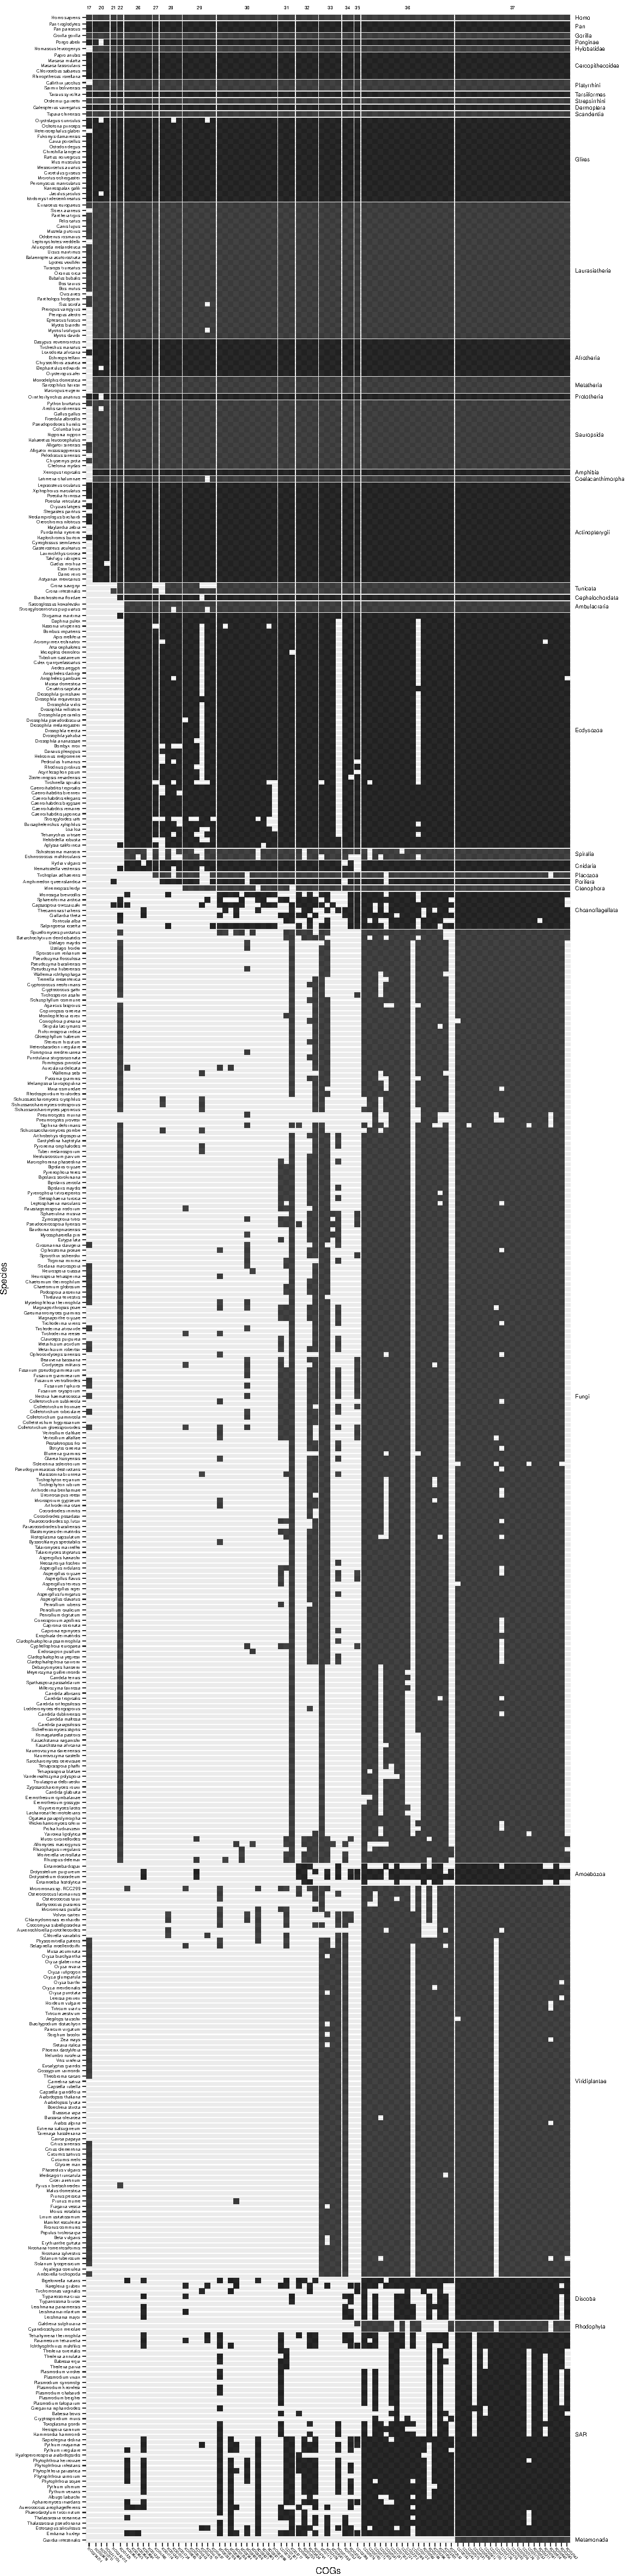
\includegraphics[height=31in, width=7in]{figs/analysis.geneplast.phyletic_patterns-1} }

\end{figure}

\clearpage

\pdfpageheight=11in

\hypertarget{adhesion-genes}{%
\subsubsection{Adhesion genes}\label{adhesion-genes}}

Aditionally\ldots{}

\begin{Shaded}
\begin{Highlighting}[]
\KeywordTok{data}\NormalTok{(}
\NormalTok{  adhesion_genes,}
\NormalTok{  gene_cogs_extra,}
  \DataTypeTok{package =} \StringTok{"neurotransmissionevolution"}
\NormalTok{)}

\NormalTok{cogs_of_interest_extra <-}\StringTok{ }\NormalTok{gene_cogs_extra }\OperatorTok\StringTok{ }\KeywordTok{pull}\NormalTok{(cog_id) }\OperatorTok\StringTok{ }\NormalTok{unique}

\NormalTok{ogr_extra <-}\StringTok{ }\KeywordTok{groot.preprocess}\NormalTok{(}
  \DataTypeTok{cogdata   =}\NormalTok{ cogs,}
  \DataTypeTok{phyloTree =}\NormalTok{ phyloTree,}
  \DataTypeTok{spid      =} \StringTok{"9606"}\NormalTok{,}
  \DataTypeTok{cogids    =}\NormalTok{ cogs_of_interest_extra}
\NormalTok{)}

\NormalTok{roots_extra <-}\StringTok{ }\KeywordTok{groot}\NormalTok{(ogr_extra, }\DataTypeTok{nPermutations =} \DecValTok{1}\NormalTok{) }\OperatorTok
\StringTok{  }\KeywordTok{groot.get}\NormalTok{(}\StringTok{"results"}\NormalTok{) }\OperatorTok
\StringTok{  }\KeywordTok{rownames_to_column}\NormalTok{(}\StringTok{"cog_id"}\NormalTok{) }\OperatorTok
\StringTok{  }\KeywordTok{left_join}\NormalTok{(gene_cogs_extra) }\OperatorTok
\StringTok{  }\KeywordTok{left_join}\NormalTok{(adhesion_genes) }\OperatorTok
\StringTok{  }\KeywordTok{left_join}\NormalTok{(lca_names, }\DataTypeTok{by =} \KeywordTok{c}\NormalTok{(}\StringTok{"Root"}\NormalTok{ =}\StringTok{ "lca"}\NormalTok{))}
\end{Highlighting}
\end{Shaded}

\begin{table}[H]

\caption{\label{tab:unnamed-chunk-8}Adhesion genes in the neural system (KEGG Pathway hsa04514).}
\begin{tabular}[t]{llll}
\toprule
String ID & COG & Symbol & Root\\
\midrule
\rowcolor{gray!6}  ENSP00000329797 & NOG10515 & CADM1 & Human-Actinopterygii LCA (\#20)\\
ENSP00000432943 & NOG16799 & MPZ & Human-Actinopterygii LCA (\#20)\\
\rowcolor{gray!6}  ENSP00000352513 & NOG16799 & MPZL1 & Human-Actinopterygii LCA (\#20)\\
ENSP00000361818 & NOG22019 & SDC4 & Human-Actinopterygii LCA (\#20)\\
\rowcolor{gray!6}  ENSP00000357106 & NOG09962 & CADM3 & Human-Tunicata LCA (\#21)\\
ENSP00000264025 & NOG09962 & NECTIN1 & Human-Tunicata LCA (\#21)\\
\rowcolor{gray!6}  ENSP00000418070 & NOG09962 & NECTIN3 & Human-Tunicata LCA (\#21)\\
ENSP00000370542 & NOG05154 & SDC1 & Human-Ambulacraria LCA (\#23)\\
\rowcolor{gray!6}  ENSP00000307046 & NOG05154 & SDC2 & Human-Ambulacraria LCA (\#23)\\
ENSP00000344468 & NOG05154 & SDC3 & Human-Ambulacraria LCA (\#23)\\
\rowcolor{gray!6}  ENSP00000265077 & NOG02372 & VCAN & Human-Cnidaria LCA (\#26)\\
ENSP00000264638 & KOG3516 & CNTNAP1 & Human-Placozoa LCA (\#27)\\
\rowcolor{gray!6}  ENSP00000354778 & KOG3516 & CNTNAP2 & Human-Placozoa LCA (\#27)\\
ENSP00000359085 & KOG3512 & NTNG1 & Human-Placozoa LCA (\#27)\\
\rowcolor{gray!6}  ENSP00000376921 & KOG3512 & NTNG2 & Human-Placozoa LCA (\#27)\\
ENSP00000447006 & KOG3513 & CNTN1 & Human-Ctenophora LCA (\#29)\\
\rowcolor{gray!6}  ENSP00000330633 & KOG3513 & CNTN2 & Human-Ctenophora LCA (\#29)\\
ENSP00000359077 & KOG3513 & L1CAM & Human-Ctenophora LCA (\#29)\\
\rowcolor{gray!6}  ENSP00000344786 & KOG3513 & NFASC & Human-Ctenophora LCA (\#29)\\
ENSP00000368314 & KOG3513 & NRCAM & Human-Ctenophora LCA (\#29)\\
\rowcolor{gray!6}  ENSP00000261769 & KOG3594 & CDH1 & Human-Unicellular holozoans LCA (\#30)\\
ENSP00000269141 & KOG3594 & CDH2 & Human-Unicellular holozoans LCA (\#30)\\
\rowcolor{gray!6}  ENSP00000379350 & KOG1226 & ITGB1 & Human-Unicellular holozoans LCA (\#30)\\
ENSP00000222573 & KOG1226 & ITGB8 & Human-Unicellular holozoans LCA (\#30)\\
\rowcolor{gray!6}  ENSP00000480132 & KOG3510 & NCAM1 & Human-Unicellular holozoans LCA (\#30)\\
ENSP00000383392 & KOG3510 & NCAM2 & Human-Unicellular holozoans LCA (\#30)\\
\rowcolor{gray!6}  ENSP00000350364 & KOG3510 & NEGR1 & Human-Unicellular holozoans LCA (\#30)\\
ENSP00000385142 & KOG3514 & NRXN1 & Human-Unicellular holozoans LCA (\#30)\\
\rowcolor{gray!6}  ENSP00000265459 & KOG3514 & NRXN2 & Human-Unicellular holozoans LCA (\#30)\\
ENSP00000451648 & KOG3514 & NRXN3 & Human-Unicellular holozoans LCA (\#30)\\
\rowcolor{gray!6}  ENSP00000367316 & KOG3637 & ITGA8 & Human-Amoebozoa LCA (\#32)\\
ENSP00000261023 & KOG3637 & ITGAV & Human-Amoebozoa LCA (\#32)\\
\rowcolor{gray!6}  ENSP00000376048 & KOG4475 & MAG & Human-Discoba LCA (\#34)\\
ENSP00000392500 & COG2272 & NLGN1 & Human-SAR LCA (\#36)\\
\rowcolor{gray!6}  ENSP00000305288 & COG2272 & NLGN2 & Human-SAR LCA (\#36)\\
ENSP00000351591 & COG2272 & NLGN3 & Human-SAR LCA (\#36)\\
\rowcolor{gray!6}  ENSP00000370485 & COG2272 & NLGN4X & Human-SAR LCA (\#36)\\
ENSP00000249363 & COG4886 & LRRC4 & Human-Metamonada LCA (\#37)\\
\rowcolor{gray!6}  ENSP00000471502 & COG4886 & LRRC4B & Human-Metamonada LCA (\#37)\\
ENSP00000278198 & COG4886 & LRRC4C & Human-Metamonada LCA (\#37)\\
\rowcolor{gray!6}  ENSP00000353030 & COG5599 & PTPRF & Human-Metamonada LCA (\#37)\\
ENSP00000463325 & COG5599 & PTPRM & Human-Metamonada LCA (\#37)\\
\bottomrule
\end{tabular}
\end{table}


\hypertarget{neuroexclusivity-1}{%
\subsection{Neuroexclusivity}\label{neuroexclusivity-1}}

We characterize genes' relevance to the nervous system by inspecting
what proportion of its activity is related to nervous processes. We
relied on tissue RNA-Seq data, as well as KEGG's pathways themselves.
Loading resources.

\begin{Shaded}
\begin{Highlighting}[]
\KeywordTok{library}\NormalTok{(tidyverse)}
\KeywordTok{library}\NormalTok{(magrittr)}

\KeywordTok{data}\NormalTok{(}
\NormalTok{   gene_ids}
\NormalTok{  ,gene_pathways}
\NormalTok{  ,gene_expression}
\NormalTok{  ,}\DataTypeTok{package =} \StringTok{"neurotransmissionevolution"}
\NormalTok{)}
\end{Highlighting}
\end{Shaded}

\hypertarget{expression-neuroexclusivity}{%
\subsubsection{Expression
neuroexclusivity}\label{expression-neuroexclusivity}}

We start by averaging all \texttt{gene\_expression} collected from the
Expression Atlas by tissue (\texttt{tpm\_avg}). The averaged expression
is filtered for values greather than 0.5 TPM. This ensures further
computations only account for tissues in which genes are actually
expressed. Then, we add the manual tissue classification indicating
which tissues are nervous or not (described in Preprocessing). The
neuroexclusivity index for a gene is the sum of its \texttt{tpm\_avg}
values in nervous tissues divided by the sum its values in all tissues.

\begin{Shaded}
\begin{Highlighting}[]
\NormalTok{tissue_classification <-}\StringTok{ }\KeywordTok{read_tsv}\NormalTok{(}
  \DataTypeTok{file      =} \StringTok{"../data/neuroexclusivity_classification_tissue.tsv"}
\NormalTok{ ,}\DataTypeTok{col_types =} \StringTok{"ci"}
\NormalTok{)}

\CommentTok{# Averaging TPM expression by tissue}
\NormalTok{avg_by_tissue <-}\StringTok{ }\NormalTok{gene_expression }\OperatorTok
\StringTok{  }\KeywordTok{group_by}\NormalTok{(ensembl_id, tissue) }\OperatorTok
\StringTok{  }\KeywordTok{summarise}\NormalTok{(}\DataTypeTok{tpm_avg =} \KeywordTok{mean}\NormalTok{(tpm)) }\OperatorTok
\StringTok{  }\KeywordTok{filter}\NormalTok{(tpm_avg }\OperatorTok{>=}\StringTok{ }\FloatTok{0.5}\NormalTok{) }\OperatorTok
\StringTok{  }\KeywordTok{left_join}\NormalTok{(tissue_classification)}

\CommentTok{# Measuring expression neuroexclusivity}
\NormalTok{expression_neuroexclusivity <-}\StringTok{ }\NormalTok{avg_by_tissue }\OperatorTok
\StringTok{  }\KeywordTok{group_by}\NormalTok{(ensembl_id) }\OperatorTok
\StringTok{  }\KeywordTok{summarise}\NormalTok{(}\DataTypeTok{expression_neuroexclusivity =} \KeywordTok{sum}\NormalTok{(tpm_avg[is_nervous }\OperatorTok{==}\StringTok{ }\DecValTok{1}\NormalTok{])}\OperatorTok{/}\KeywordTok{sum}\NormalTok{(tpm_avg)) }\OperatorTok
\StringTok{  }\KeywordTok{write_tsv}\NormalTok{(}\StringTok{"neuroexclusivity_expression.tsv"}\NormalTok{)}
\end{Highlighting}
\end{Shaded}

\hypertarget{pathway-neuroexclusivity}{%
\subsubsection{Pathway
neuroexclusivity}\label{pathway-neuroexclusivity}}

To find the pathway neuroexclusivity of a gene, we simply divide the
count of nervous pathways by the count of all pathways it participates
in.

\begin{Shaded}
\begin{Highlighting}[]
\NormalTok{pathway_classification <-}\StringTok{ }\KeywordTok{read_tsv}\NormalTok{(}
   \DataTypeTok{file      =} \StringTok{"../data/neuroexclusivity_classification_pathway.tsv"}
\NormalTok{  ,}\DataTypeTok{col_types =} \StringTok{"cci"}
\NormalTok{)}

\NormalTok{link_pathway_entrez <-}\StringTok{ }\KeywordTok{read_tsv}\NormalTok{(}
   \DataTypeTok{file      =} \StringTok{"../data-raw/download/link_pathway_entrez.tsv"}
\NormalTok{  ,}\DataTypeTok{col_names =} \KeywordTok{c}\NormalTok{(}\StringTok{"entrez_id"}\NormalTok{, }\StringTok{"pathway_id"}\NormalTok{)}
\NormalTok{  ,}\DataTypeTok{col_types =} \StringTok{"cc"}
\NormalTok{)}

\CommentTok{# Removing "hsa:" prefix}
\NormalTok{link_pathway_entrez[[}\StringTok{"entrez_id"}\NormalTok{]] }\OperatorTok\StringTok{ }\KeywordTok{str_split_n}\NormalTok{(}\StringTok{"}\CharTok{\textbackslash{}\textbackslash{}}\StringTok{:"}\NormalTok{, }\DecValTok{2}\NormalTok{)}

\CommentTok{# Pathway data related to our genes of interest}
\NormalTok{selected_genes_pathways <-}\StringTok{ }\NormalTok{link_pathway_entrez }\OperatorTok
\StringTok{  }\KeywordTok{filter}\NormalTok{(entrez_id }\OperatorTok\StringTok{ }\NormalTok{gene_ids[[}\StringTok{"entrez_id"}\NormalTok{]]) }\OperatorTok
\StringTok{  }\KeywordTok{left_join}\NormalTok{(pathway_classification) }\OperatorTok
\StringTok{  }\NormalTok{drop_na }\CommentTok{# Dropping general pathways}

\CommentTok{# Measuring pathway neuroexclusivity}
\NormalTok{pathway_neuroexclusivity <-}\StringTok{ }\NormalTok{selected_genes_pathways }\OperatorTok
\StringTok{  }\KeywordTok{group_by}\NormalTok{(entrez_id) }\OperatorTok
\StringTok{  }\KeywordTok{summarise}\NormalTok{(}\DataTypeTok{pathway_neuroexclusivity =} \KeywordTok{sum}\NormalTok{(is_nervous)}\OperatorTok{/}\KeywordTok{length}\NormalTok{(is_nervous)) }\OperatorTok
\StringTok{  }\KeywordTok{write_tsv}\NormalTok{(}\StringTok{"neuroexclusivity_pathway.tsv"}\NormalTok{)}
\end{Highlighting}
\end{Shaded}



\hypertarget{network-1}{%
\subsection{Network}\label{network-1}}

In this section we search the STRING API for our proteins of interest
and recompute the combined interaction score.
\hypertarget{graph-data}{%
\subsubsection{Graph data}\label{graph-data}}

Loading resources:

\begin{Shaded}
\begin{Highlighting}[]
\CommentTok{# Data manipulation}
\KeywordTok{library}\NormalTok{(tidyverse)}
\KeywordTok{library}\NormalTok{(igraph)}
\KeywordTok{library}\NormalTok{(magrittr)}
\KeywordTok{library}\NormalTok{(fuzzyjoin)}

\CommentTok{# Plotting dependencies}
\KeywordTok{library}\NormalTok{(scatterpie)}
\KeywordTok{library}\NormalTok{(UpSetR)}
\KeywordTok{library}\NormalTok{(gridExtra)}
\KeywordTok{library}\NormalTok{(patchwork)}

\CommentTok{# Utils}
\KeywordTok{library}\NormalTok{(neurotransmissionevolution)}

\CommentTok{# Packaged data}
\KeywordTok{data}\NormalTok{(}
\NormalTok{   gene_ids}
\NormalTok{  ,gene_cogs}
\NormalTok{  ,gene_pathways}
\NormalTok{  ,string_edgelist}
\NormalTok{  ,}\DataTypeTok{package =} \StringTok{"neurotransmissionevolution"}
\NormalTok{)}

\CommentTok{# Fresh analysis data}
\NormalTok{cog_roots                   <-}\StringTok{ }\KeywordTok{read_tsv}\NormalTok{(}\StringTok{"geneplast_roots.tsv"}\NormalTok{,             }\DataTypeTok{col_types =} \StringTok{"ci"}\NormalTok{)}
\NormalTok{clade_names                 <-}\StringTok{ }\KeywordTok{read_tsv}\NormalTok{(}\StringTok{"geneplast_clade_names.tsv"}\NormalTok{,       }\DataTypeTok{col_types =} \StringTok{"ic"}\NormalTok{)}
\NormalTok{pathway_neuroexclusivity    <-}\StringTok{ }\KeywordTok{read_tsv}\NormalTok{(}\StringTok{"neuroexclusivity_pathway.tsv"}\NormalTok{,    }\DataTypeTok{col_types =} \StringTok{"cn"}\NormalTok{)}
\NormalTok{expression_neuroexclusivity <-}\StringTok{ }\KeywordTok{read_tsv}\NormalTok{(}\StringTok{"neuroexclusivity_expression.tsv"}\NormalTok{, }\DataTypeTok{col_types =} \StringTok{"cn"}\NormalTok{)}

\CommentTok{# Collapsing similar functions}
\NormalTok{gene_annotation <-}\StringTok{ }\KeywordTok{read_tsv}\NormalTok{(}\StringTok{"../data/gene_annotation.tsv"}\NormalTok{, }\DataTypeTok{col_types =} \StringTok{"cc"}\NormalTok{) }\OperatorTok
\StringTok{  }\KeywordTok{mutate}\NormalTok{(}\DataTypeTok{annotation =} \KeywordTok{case_when}\NormalTok{(}
     \KeywordTok{grepl}\NormalTok{(}\StringTok{"clearance"}\NormalTok{,   annotation) }\OperatorTok{~}\StringTok{ "depletion"}
\NormalTok{    ,}\KeywordTok{grepl}\NormalTok{(}\StringTok{"degradation"}\NormalTok{, annotation) }\OperatorTok{~}\StringTok{ "depletion"}
\NormalTok{    ,}\KeywordTok{grepl}\NormalTok{(}\StringTok{"transport"}\NormalTok{,   annotation) }\OperatorTok{~}\StringTok{ "synthesis"}
\NormalTok{    ,}\OtherTok{TRUE} \OperatorTok{~}\StringTok{ }\NormalTok{annotation}
\NormalTok{  ))}
\end{Highlighting}
\end{Shaded}

We start by joining all gene data and creating the graph object.

\begin{Shaded}
\begin{Highlighting}[]
\CommentTok{# If a gene has more than 1 COG, select the oldest one.}
\CommentTok{# This is unusual, but can happen in cases of gene fusion, for instance.}
\NormalTok{gene_cogs }\OperatorTok
\StringTok{  }\KeywordTok{inner_join}\NormalTok{(cog_roots) }\OperatorTok
\StringTok{  }\KeywordTok{group_by}\NormalTok{(string_id) }\OperatorTok
\StringTok{  }\KeywordTok{filter}\NormalTok{(root }\OperatorTok{==}\StringTok{ }\KeywordTok{max}\NormalTok{(root)) }\OperatorTok
\StringTok{  }\KeywordTok{inner_join}\NormalTok{(clade_names)}

\CommentTok{# Gathering all gene info available}
\NormalTok{vertices <-}\StringTok{ }\NormalTok{gene_ids }\OperatorTok
\StringTok{  }\NormalTok{na.omit }\OperatorTok
\StringTok{  }\KeywordTok{inner_join}\NormalTok{(gene_cogs) }\OperatorTok
\StringTok{  }\KeywordTok{inner_join}\NormalTok{(gene_pathways) }\OperatorTok
\StringTok{  }\KeywordTok{inner_join}\NormalTok{(gene_annotation) }\OperatorTok
\StringTok{  }\KeywordTok{inner_join}\NormalTok{(pathway_neuroexclusivity) }\OperatorTok
\StringTok{  }\KeywordTok{inner_join}\NormalTok{(expression_neuroexclusivity) }\OperatorTok
\StringTok{  }\KeywordTok{mutate}\NormalTok{(}\DataTypeTok{ne =}\NormalTok{ pathway_neuroexclusivity }\OperatorTok{>=}\StringTok{ }\FloatTok{0.9}\NormalTok{) }\OperatorTok
\StringTok{  }\KeywordTok{select}\NormalTok{(string_id, }\KeywordTok{everything}\NormalTok{())}

\CommentTok{# Quick color hack to aid visualization}
\NormalTok{vertices }\OperatorTok
\StringTok{  }\KeywordTok{unite}\NormalTok{(color, glutamatergic}\OperatorTok{:}\NormalTok{dopaminergic, }\DataTypeTok{remove =}\NormalTok{ F) }\OperatorTok
\StringTok{  }\KeywordTok{mutate}\NormalTok{(}\DataTypeTok{color =} \KeywordTok{rainbow}\NormalTok{(color }\OperatorTok\StringTok{ }\NormalTok{n_distinct)[color }\OperatorTok\StringTok{ }\NormalTok{as.factor])}

\NormalTok{g <-}\StringTok{ }\KeywordTok{graph_from_data_frame}\NormalTok{(string_edgelist, }\DataTypeTok{directed =}\NormalTok{ F, }\DataTypeTok{vertices =}\NormalTok{ vertices)}

\CommentTok{# Setting node sizes}
\KeywordTok{V}\NormalTok{(g)}\OperatorTok{$}\NormalTok{size <-}\StringTok{ }\KeywordTok{V}\NormalTok{(g)}\OperatorTok{$}\NormalTok{system_count }\OperatorTok\StringTok{ }\NormalTok{sqrt }\OperatorTok\StringTok{ }\KeywordTok{multiply_by}\NormalTok{(}\DecValTok{5}\NormalTok{)}
\end{Highlighting}
\end{Shaded}

The following block calls an utility function that handles the force
directed layout with the aid of a shiny web server and the VivaGraphJS
javascript library. A computed layout is already available in this
folder.

\begin{Shaded}
\begin{Highlighting}[]
\ControlFlowTok{if}\NormalTok{(}\KeywordTok{file.exists}\NormalTok{(}\StringTok{"network_layout.tsv"}\NormalTok{)) \{}
\NormalTok{  layout <-}\StringTok{ }\KeywordTok{read_tsv}\NormalTok{(}\StringTok{"network_layout.tsv"}\NormalTok{, }\DataTypeTok{col_types =} \StringTok{"dd"}\NormalTok{) }\OperatorTok\StringTok{ }\NormalTok{as.matrix}
\NormalTok{\} }\ControlFlowTok{else}\NormalTok{ \{}
\NormalTok{  layout <-}\StringTok{ }\KeywordTok{vivagraph}\NormalTok{(g, }\DataTypeTok{precompute_multiplier =} \DecValTok{200}\NormalTok{, }\DataTypeTok{precompute_niter =} \DecValTok{1000}\NormalTok{)}
\NormalTok{\}}

\CommentTok{# inserting layout coordinates into graph object}
\KeywordTok{V}\NormalTok{(g)}\OperatorTok{$}\NormalTok{x <-}\StringTok{  }\NormalTok{layout[, }\DecValTok{1}\NormalTok{]}
\CommentTok{# layout matrix comes vertically flipped}
\KeywordTok{V}\NormalTok{(g)}\OperatorTok{$}\NormalTok{y <-}\StringTok{ }\OperatorTok{-}\NormalTok{layout[, }\DecValTok{2}\NormalTok{]}
\end{Highlighting}
\end{Shaded}

We use base ggplot2 to draw the network. Edges are represented by a
common \texttt{geom\_path} layer. The following block retrieves tidy
edge coordinates for the \texttt{geom\_path} calls.

\begin{Shaded}
\begin{Highlighting}[]
\CommentTok{# Recreating the vertices data.frame, now with layout coordinates (lazy way)}
\NormalTok{vertices <-}\StringTok{ }\NormalTok{igraph}\OperatorTok{::}\KeywordTok{as_data_frame}\NormalTok{(g, }\DataTypeTok{what =} \StringTok{"vertices"}\NormalTok{) }\OperatorTok\StringTok{ }\KeywordTok{rename}\NormalTok{(}\DataTypeTok{string_id =}\NormalTok{ name)}

\CommentTok{# The edges and edges_long data.frames will be used to draw lines with geom_path}
\NormalTok{edges <-}\StringTok{ }\NormalTok{string_edgelist }\OperatorTok
\StringTok{    }\KeywordTok{map}\NormalTok{(match, vertices[[}\StringTok{"string_id"}\NormalTok{]]) }\OperatorTok
\StringTok{    }\KeywordTok{map_dfr}\NormalTok{(}\OperatorTok{~}\StringTok{ }\NormalTok{vertices[.x,]) }\OperatorTok
\StringTok{    }\KeywordTok{select}\NormalTok{(x, y, string_id) }\OperatorTok
\StringTok{    }\KeywordTok{cbind}\NormalTok{(}\DataTypeTok{group =} \DecValTok{1}\OperatorTok{:}\KeywordTok{nrow}\NormalTok{(string_edgelist))}

\NormalTok{edges_long <-}\StringTok{ }\NormalTok{string_edgelist }\OperatorTok
\StringTok{  }\KeywordTok{data.frame}\NormalTok{(}
     \DataTypeTok{string_id        =} \KeywordTok{c}\NormalTok{(stringId_A, stringId_B)}
\NormalTok{    ,}\DataTypeTok{group            =} \DecValTok{1}\OperatorTok{:}\KeywordTok{nrow}\NormalTok{(.)}
\NormalTok{    ,}\DataTypeTok{stringsAsFactors =} \OtherTok{FALSE}
\NormalTok{  )}
\end{Highlighting}
\end{Shaded}

Setting up reusable aesthetic parameters to avoid code duplication.

\begin{Shaded}
\begin{Highlighting}[]
\NormalTok{systems <-}\StringTok{ }\KeywordTok{c}\NormalTok{(}
   \StringTok{"cholinergic"}
\NormalTok{  ,}\StringTok{"dopaminergic"}
\NormalTok{  ,}\StringTok{"gabaergic"}
\NormalTok{  ,}\StringTok{"glutamatergic"}
\NormalTok{  ,}\StringTok{"serotonergic"}
\NormalTok{)}
\NormalTok{systems_labeller <-}\StringTok{ }\KeywordTok{c}\NormalTok{(}
   \StringTok{"Cholinergic"}\NormalTok{   =}\StringTok{ "cholinergic"}
\NormalTok{  ,}\StringTok{"Dopaminergic"}\NormalTok{  =}\StringTok{ "dopaminergic"}
\NormalTok{  ,}\StringTok{"GABAergic"}\NormalTok{     =}\StringTok{ "gabaergic"}
\NormalTok{  ,}\StringTok{"Glutamatergic"}\NormalTok{ =}\StringTok{ "glutamatergic"}
\NormalTok{  ,}\StringTok{"Serotonergic"}\NormalTok{  =}\StringTok{ "serotonergic"}
\NormalTok{)}

\NormalTok{edge_color <-}\StringTok{ }\KeywordTok{rgb}\NormalTok{(}\FloatTok{0.7}\NormalTok{, }\FloatTok{0.7}\NormalTok{, }\FloatTok{0.7}\NormalTok{, }\DataTypeTok{alpha =} \FloatTok{0.3}\NormalTok{)}

\NormalTok{color_mappings <-}\StringTok{ }\KeywordTok{c}\NormalTok{(}
  \CommentTok{#----- neurotransmitter systems ----}
   \StringTok{"cholinergic"}\NormalTok{           =}\StringTok{ "#D84315"}
\NormalTok{  ,}\StringTok{"dopaminergic"}\NormalTok{          =}\StringTok{ "#F9A825"}
\NormalTok{  ,}\StringTok{"gabaergic"}\NormalTok{             =}\StringTok{ "#558B2F"}
\NormalTok{  ,}\StringTok{"glutamatergic"}\NormalTok{         =}\StringTok{ "#1565C0"}
\NormalTok{  ,}\StringTok{"serotonergic"}\NormalTok{          =}\StringTok{ "#6A1B9A"}
  \CommentTok{#--- neurotransmission functions ---}
\NormalTok{  ,}\StringTok{"depletion"}\NormalTok{             =}\StringTok{ "#F40000"}
\NormalTok{  ,}\StringTok{"excitability"}\NormalTok{          =}\StringTok{ "#FFAB00"}
\NormalTok{  ,}\StringTok{"receptor-associated"}\NormalTok{   =}\StringTok{ "#D6EE00"}
\NormalTok{  ,}\StringTok{"ionotropic receptor"}\NormalTok{   =}\StringTok{ "#43FF1C"}
\NormalTok{  ,}\StringTok{"metabotropic receptor"}\NormalTok{ =}\StringTok{ "#18FFFF"}
\NormalTok{  ,}\StringTok{"signaling"}\NormalTok{             =}\StringTok{ "#0091EA"}
\NormalTok{  ,}\StringTok{"g-protein"}\NormalTok{             =}\StringTok{ "#0033ff"}
\NormalTok{  ,}\StringTok{"synthesis"}\NormalTok{             =}\StringTok{ "#AA00FF"}
\NormalTok{  ,}\StringTok{"vesicle"}\NormalTok{               =}\StringTok{ "#FF00AA"}
  \CommentTok{#------- is_neuroexclusive ---------}
\NormalTok{  ,}\StringTok{"TRUE"}\NormalTok{                  =}\StringTok{ "#00BFC4"}
\NormalTok{  ,}\StringTok{"FALSE"}\NormalTok{                 =}\StringTok{ "#F8766D"}
  \CommentTok{#-------- network faceting ---------}
\NormalTok{  ,}\StringTok{"past"}\NormalTok{                  =}\StringTok{ "#FFFFFF"}
\NormalTok{  ,}\StringTok{"other"}\NormalTok{                 =}\StringTok{ "#A0A0A0"}
\NormalTok{  ,}\StringTok{"other_edge"}\NormalTok{            =}\StringTok{ }\KeywordTok{rgb}\NormalTok{(}\FloatTok{0.7}\NormalTok{, }\FloatTok{0.7}\NormalTok{, }\FloatTok{0.7}\NormalTok{)}
\NormalTok{  ,}\StringTok{"ne_border"}\NormalTok{             =}\StringTok{ "#000000"}
\NormalTok{)}

\NormalTok{node_fill_scale  <-}\StringTok{ }\KeywordTok{scale_fill_manual}\NormalTok{(}\DataTypeTok{values =}\NormalTok{ color_mappings)}
\NormalTok{node_color_scale <-}\StringTok{ }\KeywordTok{scale_color_manual}\NormalTok{(}\DataTypeTok{values =}\NormalTok{ color_mappings }\OperatorTok\StringTok{ }\KeywordTok{darken}\NormalTok{(}\FloatTok{0.2}\NormalTok{))}

\CommentTok{# Color and size scales for neurotransmission functions}
\NormalTok{plot_scales <-}\StringTok{ }\KeywordTok{list}\NormalTok{(}
\NormalTok{   node_fill_scale}
\NormalTok{  ,node_color_scale}
\NormalTok{  ,}\KeywordTok{scale_radius}\NormalTok{(}\DataTypeTok{range =} \KeywordTok{c}\NormalTok{(}\FloatTok{1.75}\NormalTok{, }\FloatTok{5.00}\NormalTok{), }\DataTypeTok{guide =} \OtherTok{FALSE}\NormalTok{)}
\NormalTok{)}

\NormalTok{past_fill  <-}\StringTok{ "#FFFFFF"} \CommentTok{# past nodes' fill color}
\NormalTok{past_color <-}\StringTok{ "#888888"} \CommentTok{# past nodes' border color}

\CommentTok{# Baking some aesthetic properties into the vertices data.frame}
\NormalTok{vertices }\OperatorTok\StringTok{ }\KeywordTok{mutate}\NormalTok{(}
  \DataTypeTok{shape      =} \KeywordTok{ifelse}\NormalTok{(ne, }\StringTok{"square filled"}\NormalTok{, }\StringTok{"circle filled"}\NormalTok{),}
  \DataTypeTok{color_node =} \KeywordTok{ifelse}\NormalTok{(ne, }\StringTok{"#000000"}\NormalTok{, color_mappings[annotation] }\OperatorTok\StringTok{ }\KeywordTok{darken}\NormalTok{(}\FloatTok{0.2}\NormalTok{)),}
  \DataTypeTok{color_pie  =} \KeywordTok{ifelse}\NormalTok{(ne, }\StringTok{"#000000"}\NormalTok{, }\OtherTok{NA}\NormalTok{),}
\NormalTok{)}

\CommentTok{# Some recurrent ggplot aesthetics}
\NormalTok{edge_aes <-}\StringTok{ }\KeywordTok{aes}\NormalTok{(}\DataTypeTok{x =}\NormalTok{ x, }\DataTypeTok{y =}\NormalTok{ y, }\DataTypeTok{group =}\NormalTok{ group)}
\NormalTok{text_aes <-}\StringTok{ }\KeywordTok{aes}\NormalTok{(}\DataTypeTok{x =}\NormalTok{ x, }\DataTypeTok{y =}\NormalTok{ y, }\DataTypeTok{label =}\NormalTok{ string_name)}
\NormalTok{pie_aes  <-}\StringTok{ }\KeywordTok{aes}\NormalTok{(}\DataTypeTok{x =}\NormalTok{ x, }\DataTypeTok{y =}\NormalTok{ y, }\DataTypeTok{group =}\NormalTok{ string_id, }\DataTypeTok{r =}\NormalTok{ size}\OperatorTok{^}\NormalTok{(}\FloatTok{0.94}\NormalTok{) }\OperatorTok{-}\StringTok{ }\FloatTok{1.5}\NormalTok{)}

\CommentTok{# Fixing xy limits across all plots}
\NormalTok{xy_lim <-}\StringTok{ }\KeywordTok{list}\NormalTok{(}
  \KeywordTok{scale_x_continuous}\NormalTok{(}\DataTypeTok{limits =} \KeywordTok{range}\NormalTok{(vertices[[}\StringTok{"x"}\NormalTok{]]) }\OperatorTok{+}\StringTok{ }\KeywordTok{c}\NormalTok{(}\OperatorTok{-}\DecValTok{50}\NormalTok{, }\DecValTok{50}\NormalTok{)),}
  \KeywordTok{scale_y_continuous}\NormalTok{(}\DataTypeTok{limits =} \KeywordTok{range}\NormalTok{(vertices[[}\StringTok{"y"}\NormalTok{]]) }\OperatorTok{+}\StringTok{ }\KeywordTok{c}\NormalTok{(}\OperatorTok{-}\DecValTok{50}\NormalTok{, }\DecValTok{50}\NormalTok{))}
\NormalTok{)}

\CommentTok{# Emptying theme defaults}
\NormalTok{plot_theme <-}\StringTok{ }\KeywordTok{list}\NormalTok{(}\KeywordTok{coord_equal}\NormalTok{(), }\KeywordTok{theme_void}\NormalTok{())}

\CommentTok{# Allowing more space for multiple network plots}
\NormalTok{diff_theme <-}\StringTok{ }\KeywordTok{list}\NormalTok{(}
  \KeywordTok{coord_equal}\NormalTok{(),}
  \KeywordTok{theme_void}\NormalTok{(),}
  \KeywordTok{theme}\NormalTok{(}
     \DataTypeTok{plot.title         =} \KeywordTok{element_text}\NormalTok{(}\DataTypeTok{size =} \DecValTok{8}\NormalTok{, }\DataTypeTok{hjust =} \FloatTok{0.5}\NormalTok{)}
\NormalTok{    ,}\DataTypeTok{legend.text        =} \KeywordTok{element_text}\NormalTok{(}\DataTypeTok{size =} \DecValTok{6}\NormalTok{)}
\NormalTok{    ,}\DataTypeTok{legend.title       =} \KeywordTok{element_text}\NormalTok{(}\DataTypeTok{size =} \DecValTok{8}\NormalTok{)}
\NormalTok{    ,}\DataTypeTok{legend.key.size    =} \KeywordTok{unit}\NormalTok{( }\DecValTok{1}\NormalTok{, }\StringTok{"mm"}\NormalTok{)}
\NormalTok{    ,}\DataTypeTok{legend.box.spacing =} \KeywordTok{unit}\NormalTok{(}\OperatorTok{-}\DecValTok{2}\NormalTok{, }\StringTok{"mm"}\NormalTok{)}
\NormalTok{    ,}\DataTypeTok{legend.box.margin  =} \KeywordTok{unit}\NormalTok{(}\KeywordTok{c}\NormalTok{(}\DecValTok{0}\NormalTok{, }\DecValTok{2}\NormalTok{, }\DecValTok{0}\NormalTok{, }\DecValTok{0}\NormalTok{), }\StringTok{"mm"}\NormalTok{)}
\NormalTok{    ,}\DataTypeTok{plot.margin        =} \KeywordTok{unit}\NormalTok{(}\KeywordTok{c}\NormalTok{(}\DecValTok{0}\NormalTok{, }\DecValTok{0}\NormalTok{, }\DecValTok{0}\NormalTok{, }\DecValTok{0}\NormalTok{), }\StringTok{"mm"}\NormalTok{)}
\NormalTok{  )}
\NormalTok{)}

\CommentTok{# Numeric vector named with clade names}
\NormalTok{roots <-}\StringTok{ }\NormalTok{vertices }\OperatorTok
\StringTok{  }\KeywordTok{arrange}\NormalTok{(}\OperatorTok{-}\NormalTok{root) }\OperatorTok
\StringTok{  }\KeywordTok{distinct}\NormalTok{(root, clade_name) }\OperatorTok
\StringTok{  }\KeywordTok{set_names}\NormalTok{(root, clade_name)}

\NormalTok{upset_texts <-}\StringTok{ }\KeywordTok{c}\NormalTok{(}
   \DecValTok{3}   \CommentTok{#ytitle}
\NormalTok{  ,}\DecValTok{2}   \CommentTok{#ytick}
\NormalTok{  ,}\DecValTok{1}   \CommentTok{#setsizetitle}
\NormalTok{  ,}\FloatTok{1.5} \CommentTok{#setsizetick}
\NormalTok{  ,}\DecValTok{2}   \CommentTok{#setnames}
\NormalTok{  ,}\FloatTok{2.5} \CommentTok{#barnums}
\NormalTok{)}
\end{Highlighting}
\end{Shaded}

\hypertarget{manuscript-figure-1}{%
\subsubsection{Manuscript figure 1}\label{manuscript-figure-1}}

\begin{Shaded}
\begin{Highlighting}[]
\CommentTok{####################}
\CommentTok{## Common elements}
\CommentTok{####################}
\NormalTok{plot_edges <-}\StringTok{ }\KeywordTok{geom_path}\NormalTok{(}
   \DataTypeTok{data    =}\NormalTok{ edges}
\NormalTok{  ,}\DataTypeTok{mapping =}\NormalTok{ edge_aes}
\NormalTok{  ,}\DataTypeTok{color   =}\NormalTok{ edge_color}
\NormalTok{  ,}\DataTypeTok{size    =} \FloatTok{0.1}
\NormalTok{)}

\NormalTok{plot_text <-}\StringTok{ }\KeywordTok{geom_text}\NormalTok{(}
   \DataTypeTok{data    =}\NormalTok{ vertices}
\NormalTok{  ,}\DataTypeTok{mapping =}\NormalTok{ text_aes}
\NormalTok{  ,}\DataTypeTok{size    =} \DecValTok{1}
\NormalTok{  ,}\DataTypeTok{vjust   =} \DecValTok{0}
\NormalTok{  ,}\DataTypeTok{nudge_y =} \DecValTok{6}
\NormalTok{  ,}\DataTypeTok{alpha   =} \FloatTok{0.5}
\NormalTok{)}

\CommentTok{##############}
\CommentTok{## Figure 1A}
\CommentTok{##############}
\NormalTok{plot_pies <-}\StringTok{ }\KeywordTok{geom_scatterpie}\NormalTok{(}
   \DataTypeTok{data    =}\NormalTok{ vertices}
\NormalTok{  ,}\DataTypeTok{mapping =}\NormalTok{ pie_aes}
\NormalTok{  ,}\DataTypeTok{cols    =}\NormalTok{ systems}
\NormalTok{  ,}\DataTypeTok{color   =} \OtherTok{NA}
\NormalTok{)}

\NormalTok{fig1a <-}\StringTok{ }\KeywordTok{ggplot}\NormalTok{() }\OperatorTok{+}
\StringTok{  }\NormalTok{plot_theme }\OperatorTok{+}
\StringTok{  }\NormalTok{plot_edges }\OperatorTok{+}
\StringTok{  }\NormalTok{plot_pies }\OperatorTok{+}
\StringTok{  }\NormalTok{node_fill_scale }\OperatorTok{+}
\StringTok{  }\NormalTok{plot_text}

\CommentTok{##############}
\CommentTok{## Figure 1B}
\CommentTok{##############}
\NormalTok{plot_nodes <-}\StringTok{ }\KeywordTok{geom_point}\NormalTok{(}
   \DataTypeTok{data    =}\NormalTok{ vertices}
\NormalTok{  ,}\DataTypeTok{mapping =} \KeywordTok{aes}\NormalTok{(x, y, }\DataTypeTok{fill =}\NormalTok{ annotation, }\DataTypeTok{color =}\NormalTok{ annotation, }\DataTypeTok{size =}\NormalTok{ size)}
\NormalTok{  ,}\DataTypeTok{shape   =} \DecValTok{21}
\NormalTok{  ,}\DataTypeTok{stroke  =} \FloatTok{0.5}
\NormalTok{)}
  
\NormalTok{fig1b <-}\StringTok{ }\KeywordTok{ggplot}\NormalTok{() }\OperatorTok{+}
\StringTok{  }\NormalTok{plot_theme }\OperatorTok{+}
\StringTok{  }\NormalTok{plot_edges }\OperatorTok{+}
\StringTok{  }\NormalTok{plot_nodes }\OperatorTok{+}
\StringTok{  }\NormalTok{plot_scales }\OperatorTok{+}
\StringTok{  }\NormalTok{plot_text}

\CommentTok{# Plotting and saving}
\NormalTok{fig1a }\OperatorTok{/}\StringTok{ }\NormalTok{fig1b}
\end{Highlighting}
\end{Shaded}

\begin{Shaded}
\begin{Highlighting}[]
\CommentTok{# ggsave("plots/fig1_raw.pdf", width = 14, height = 7, onefile = F, useDingbats = F)}
\end{Highlighting}
\end{Shaded}

\clearpage

\begin{figure}
\centering
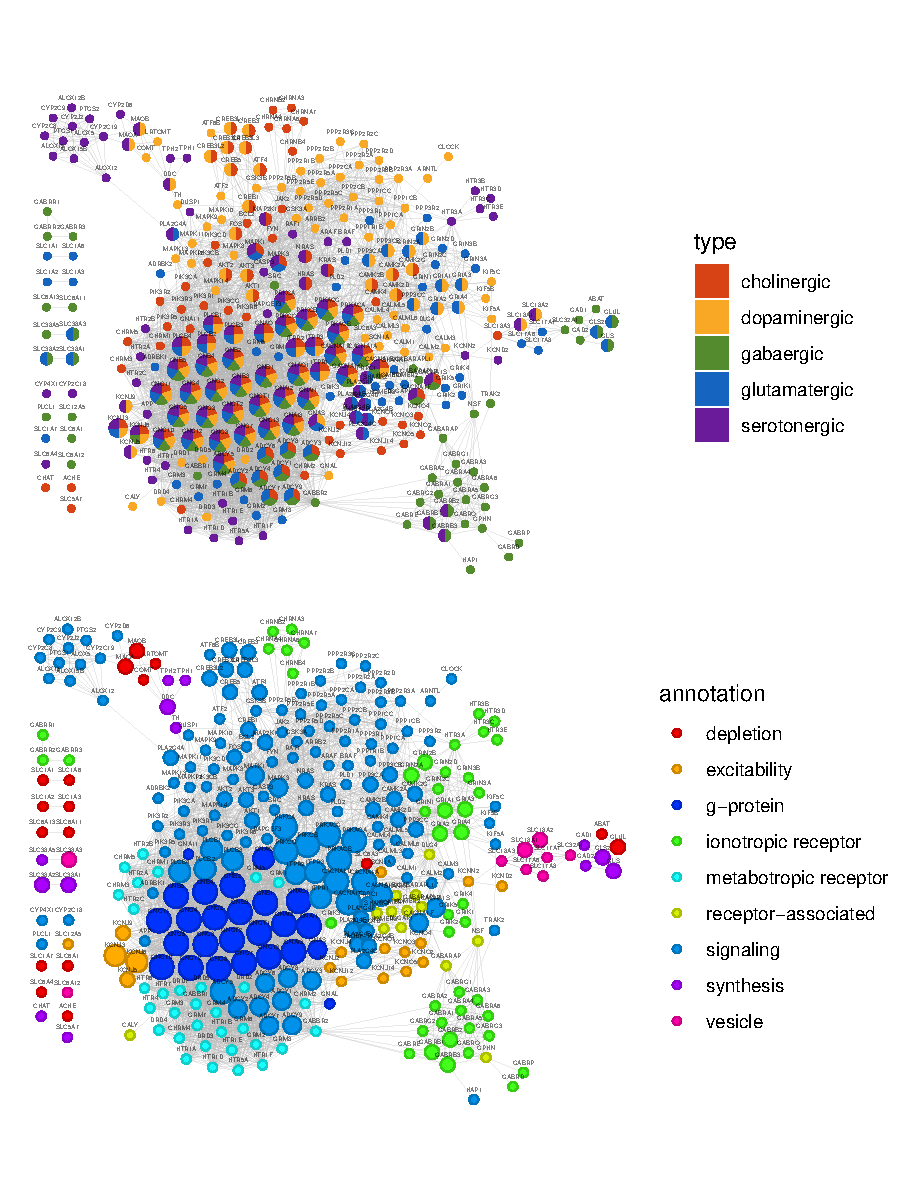
\includegraphics[width=\textwidth,height=0.9\textheight]{figs/analysis.network.fig1_raw-1}
\caption{test.}
\end{figure}

\clearpage

\hypertarget{manuscript-figure-2}{%
\subsubsection{Manuscript figure 2}\label{manuscript-figure-2}}

This figure is produced externally by a program called ViaComplex.
ViaComplex superimposes a heatmap over the network layout based on a
node property. We are going to use nodes neuroexclusivity values. The
following block handles data formatting related to ViaComplex.

\begin{Shaded}
\begin{Highlighting}[]
\CommentTok{# Retrieving the largest connected component}
\NormalTok{subgraphs <-}\StringTok{ }\KeywordTok{decompose.graph}\NormalTok{(g)}
\NormalTok{lcc_index <-}\StringTok{ }\KeywordTok{which.max}\NormalTok{(}\KeywordTok{sapply}\NormalTok{(subgraphs, vcount))}
\NormalTok{lcc       <-}\StringTok{ }\NormalTok{subgraphs[[lcc_index]]}

\CommentTok{# Writing network data to viacomplex's custom format (similar to pajek)}
\CommentTok{# xy_hack adds some extra margin to the plot}
\NormalTok{xy_hack <-}\StringTok{ }\KeywordTok{data.frame}\NormalTok{(}
   \DataTypeTok{name                        =} \KeywordTok{c}\NormalTok{(}\StringTok{"top"}\NormalTok{, }\StringTok{"bot"}\NormalTok{)}
\NormalTok{  ,}\DataTypeTok{x                           =} \KeywordTok{range}\NormalTok{(}\KeywordTok{V}\NormalTok{(lcc)}\OperatorTok{$}\NormalTok{x) }\OperatorTok{+}\StringTok{ }\KeywordTok{c}\NormalTok{(}\OperatorTok{-}\DecValTok{75}\NormalTok{, }\DecValTok{75}\NormalTok{)}
\NormalTok{  ,}\DataTypeTok{y                           =} \KeywordTok{range}\NormalTok{(}\KeywordTok{V}\NormalTok{(lcc)}\OperatorTok{$}\NormalTok{y) }\OperatorTok{+}\StringTok{ }\KeywordTok{c}\NormalTok{(}\OperatorTok{-}\DecValTok{75}\NormalTok{, }\DecValTok{75}\NormalTok{)}
\NormalTok{  ,}\DataTypeTok{pathway_neuroexclusivity    =} \DecValTok{0}
\NormalTok{  ,}\DataTypeTok{expression_neuroexclusivity =} \DecValTok{0}
\NormalTok{  ,}\DataTypeTok{stringsAsFactors            =}\NormalTok{ F}
\NormalTok{)}

\NormalTok{pajek_nodes <-}\StringTok{ }\NormalTok{lcc }\OperatorTok
\StringTok{  }\NormalTok{igraph}\OperatorTok{::}\KeywordTok{as_data_frame}\NormalTok{(}\StringTok{"vertices"}\NormalTok{) }\OperatorTok
\StringTok{  }\KeywordTok{bind_rows}\NormalTok{(xy_hack) }\OperatorTok
\StringTok{  }\KeywordTok{mutate}\NormalTok{(}\DataTypeTok{id =} \KeywordTok{row_number}\NormalTok{(), }\DataTypeTok{y =} \OperatorTok{-}\NormalTok{y)}

\NormalTok{pajek_edges <-}\StringTok{ }\NormalTok{igraph}\OperatorTok{::}\KeywordTok{as_data_frame}\NormalTok{(lcc, }\StringTok{"edges"}\NormalTok{)}

\CommentTok{# Creating the network_viacomplex.net file and sequentially populating it}
\KeywordTok{write}\NormalTok{(}\StringTok{"*edges"}\NormalTok{, }\StringTok{"network_viacomplex.net"}\NormalTok{)}
\KeywordTok{write_tsv}\NormalTok{(}
   \DataTypeTok{x            =}\NormalTok{ pajek_edges}
\NormalTok{  ,}\DataTypeTok{path         =} \StringTok{"network_viacomplex.net"}
\NormalTok{  ,}\DataTypeTok{append       =}\NormalTok{ T}
\NormalTok{  ,}\DataTypeTok{col_names    =}\NormalTok{ F}
\NormalTok{  ,}\DataTypeTok{quote_escape =}\NormalTok{ F}
\NormalTok{)}
\KeywordTok{write}\NormalTok{(}\StringTok{"*nodes"}\NormalTok{, }\StringTok{"network_viacomplex.net"}\NormalTok{, }\DataTypeTok{append =}\NormalTok{ T)}
\KeywordTok{write_tsv}\NormalTok{(}
   \DataTypeTok{x            =}\NormalTok{ pajek_nodes }\OperatorTok\StringTok{ }\KeywordTok{select}\NormalTok{(name, x, y)}
\NormalTok{  ,}\DataTypeTok{path         =} \StringTok{"network_viacomplex.net"}
\NormalTok{  ,}\DataTypeTok{append       =}\NormalTok{ T}
\NormalTok{  ,}\DataTypeTok{col_names    =}\NormalTok{ F}
\NormalTok{  ,}\DataTypeTok{quote_escape =}\NormalTok{ F}
\NormalTok{)}

\KeywordTok{write_tsv}\NormalTok{(}
   \DataTypeTok{x    =}\NormalTok{ pajek_nodes }\OperatorTok\StringTok{ }\KeywordTok{select}\NormalTok{(id, name, pathway_neuroexclusivity)}
\NormalTok{  ,}\DataTypeTok{path =} \StringTok{"network_viacomplex_pathway.dat"}
\NormalTok{)}
\KeywordTok{write_tsv}\NormalTok{(}
   \DataTypeTok{x    =}\NormalTok{ pajek_nodes }\OperatorTok\StringTok{ }\KeywordTok{select}\NormalTok{(id, name, expression_neuroexclusivity)}
\NormalTok{  ,}\DataTypeTok{path =} \StringTok{"network_viacomplex_expression.dat"}
\NormalTok{)}
\end{Highlighting}
\end{Shaded}

\hypertarget{manuscript-figure-3}{%
\subsubsection{Manuscript figure 3}\label{manuscript-figure-3}}

The process for generating Figures 3 and 4 is roughly the same. It
consists of finding what nodes have numeric roots in a given range. In
our analysis, the largest root is numbered 37 and represents the oldest
common ancestor to humans in the cladogram (the Human-Metamonada LCA, as
seen in previous sections). Root number 1 is represented by \emph{Homo
sapiens} itself.\\
The nodes we need to draw are either \texttt{current\_nodes} (roots in a
specified numeric range), or \texttt{past\_nodes} (roots \textgreater{}
such specified range). The edges we need to draw are all edges between
both sets of nodes.\\
\textbf{Manuscript Figure 3A}

\begin{Shaded}
\begin{Highlighting}[]
\CommentTok{# Finding which genes should be drawn}
\NormalTok{current_genes <-}\StringTok{ }\NormalTok{vertices }\OperatorTok\StringTok{ }\KeywordTok{filter}\NormalTok{(root }\OperatorTok{==}\StringTok{ }\DecValTok{37}\NormalTok{)}

\CommentTok{# Finding which edges should be drawn}
\NormalTok{partial_ids   <-}\StringTok{ }\NormalTok{current_genes }\OperatorTok\StringTok{ }\KeywordTok{pull}\NormalTok{(string_id)}
\NormalTok{which_edges   <-}\StringTok{ }\KeywordTok{apply}\NormalTok{(string_edgelist, }\DecValTok{1}\NormalTok{, }\ControlFlowTok{function}\NormalTok{(r) }\KeywordTok{all}\NormalTok{(r }\OperatorTok\StringTok{ }\NormalTok{partial_ids))}
\NormalTok{partial_edges <-}\StringTok{ }\NormalTok{edges[which_edges }\OperatorTok\StringTok{ }\KeywordTok{rep}\NormalTok{(}\DecValTok{2}\NormalTok{),]}

\NormalTok{plot_edges <-}\StringTok{ }\KeywordTok{geom_path}\NormalTok{(}
   \DataTypeTok{data    =}\NormalTok{ partial_edges}
\NormalTok{  ,}\DataTypeTok{mapping =}\NormalTok{ edge_aes}
\NormalTok{  ,}\DataTypeTok{color   =}\NormalTok{ edge_color}
\NormalTok{  ,}\DataTypeTok{size    =} \FloatTok{0.1}
\NormalTok{)}

\NormalTok{plot_text <-}\StringTok{ }\KeywordTok{geom_text}\NormalTok{(}
   \DataTypeTok{data    =}\NormalTok{ current_genes}
\NormalTok{  ,}\DataTypeTok{mapping =}\NormalTok{ text_aes}
\NormalTok{  ,}\DataTypeTok{size    =} \DecValTok{1}
\NormalTok{  ,}\DataTypeTok{vjust   =} \DecValTok{0}
\NormalTok{  ,}\DataTypeTok{nudge_y =} \FloatTok{1.75}
\NormalTok{  ,}\DataTypeTok{alpha   =} \FloatTok{0.5}
\NormalTok{)}

\NormalTok{plot_current_pies <-}\StringTok{ }\KeywordTok{geom_scatterpie}\NormalTok{(}
   \DataTypeTok{data    =}\NormalTok{ current_genes}
\NormalTok{  ,}\DataTypeTok{mapping =}\NormalTok{ pie_aes}
\NormalTok{  ,}\DataTypeTok{cols    =}\NormalTok{ systems}
\NormalTok{  ,}\DataTypeTok{color   =} \OtherTok{NA}
\NormalTok{)}

\CommentTok{# Assembling}
\NormalTok{fig3a <-}\StringTok{ }\KeywordTok{ggplot}\NormalTok{() }\OperatorTok{+}
\StringTok{  }\NormalTok{plot_edges }\OperatorTok{+}
\StringTok{  }\NormalTok{plot_scales }\OperatorTok{+}
\StringTok{  }\NormalTok{xy_lim }\OperatorTok{+}
\StringTok{  }\NormalTok{plot_current_pies }\OperatorTok{+}
\StringTok{  }\NormalTok{node_fill_scale }\OperatorTok{+}
\StringTok{  }\NormalTok{plot_text }\OperatorTok{+}
\StringTok{  }\NormalTok{plot_theme}
\end{Highlighting}
\end{Shaded}

\textbf{Manuscript Figure 3B}\\
For Figure 3B, we want to see what nodes have numeric roots \textless{}
37 (Human-Metamonada LCA) and \textgreater= 26 (Human-Cnidaria LCA).

\begin{Shaded}
\begin{Highlighting}[]
\CommentTok{# Finding which genes should be drawn}
\NormalTok{current_genes <-}\StringTok{ }\NormalTok{vertices }\OperatorTok\StringTok{ }\KeywordTok{filter}\NormalTok{(root }\OperatorTok{<}\StringTok{ }\DecValTok{37} \OperatorTok{&}\StringTok{ }\NormalTok{root }\OperatorTok{>=}\StringTok{ }\DecValTok{26}\NormalTok{)}
\NormalTok{past_genes    <-}\StringTok{ }\NormalTok{vertices }\OperatorTok\StringTok{ }\KeywordTok{filter}\NormalTok{(root }\OperatorTok{==}\StringTok{ }\DecValTok{37}\NormalTok{)}

\CommentTok{# Finding which edges should be drawn}
\NormalTok{partial_ids   <-}\StringTok{ }\KeywordTok{c}\NormalTok{(current_genes[[}\StringTok{"string_id"}\NormalTok{]], past_genes[[}\StringTok{"string_id"}\NormalTok{]])}
\NormalTok{which_edges   <-}\StringTok{ }\KeywordTok{apply}\NormalTok{(string_edgelist, }\DecValTok{1}\NormalTok{, }\ControlFlowTok{function}\NormalTok{(r) }\KeywordTok{all}\NormalTok{(r }\OperatorTok\StringTok{ }\NormalTok{partial_ids))}
\NormalTok{partial_edges <-}\StringTok{ }\NormalTok{edges[which_edges }\OperatorTok\StringTok{ }\KeywordTok{rep}\NormalTok{(}\DecValTok{2}\NormalTok{),]}

\NormalTok{plot_edges <-}\StringTok{ }\KeywordTok{geom_path}\NormalTok{(}
   \DataTypeTok{data    =}\NormalTok{ partial_edges}
\NormalTok{  ,}\DataTypeTok{mapping =}\NormalTok{ edge_aes}
\NormalTok{  ,}\DataTypeTok{color   =}\NormalTok{ edge_color}
\NormalTok{  ,}\DataTypeTok{size    =} \FloatTok{0.1}
\NormalTok{)}

\NormalTok{plot_past <-}\StringTok{ }\KeywordTok{geom_point}\NormalTok{(}
   \DataTypeTok{data    =}\NormalTok{ past_genes}
\NormalTok{  ,}\DataTypeTok{mapping =} \KeywordTok{aes}\NormalTok{(x, y, }\DataTypeTok{size =}\NormalTok{ size)}
\NormalTok{  ,}\DataTypeTok{fill    =}\NormalTok{ past_fill}
\NormalTok{  ,}\DataTypeTok{color   =}\NormalTok{ past_color}
\NormalTok{  ,}\DataTypeTok{shape   =}\NormalTok{ past_genes}\OperatorTok{$}\NormalTok{shape}
\NormalTok{  ,}\DataTypeTok{stroke  =} \FloatTok{0.25}
\NormalTok{)}

\NormalTok{plot_text <-}\StringTok{ }\KeywordTok{geom_text}\NormalTok{(}
   \DataTypeTok{data    =}\NormalTok{ current_genes}
\NormalTok{  ,}\DataTypeTok{mapping =}\NormalTok{ text_aes}
\NormalTok{  ,}\DataTypeTok{size    =} \DecValTok{1}
\NormalTok{  ,}\DataTypeTok{vjust   =} \DecValTok{0}
\NormalTok{  ,}\DataTypeTok{nudge_y =} \FloatTok{1.75}
\NormalTok{  ,}\DataTypeTok{alpha   =} \FloatTok{0.5}
\NormalTok{)}

\NormalTok{plot_current_pies <-}\StringTok{ }\KeywordTok{geom_scatterpie}\NormalTok{(}
   \DataTypeTok{data    =}\NormalTok{ current_genes}
\NormalTok{  ,}\DataTypeTok{mapping =}\NormalTok{ pie_aes}
\NormalTok{  ,}\DataTypeTok{cols    =}\NormalTok{ systems}
\NormalTok{  ,}\DataTypeTok{color   =} \OtherTok{NA}
\NormalTok{)}

\CommentTok{# Assembling}
\NormalTok{fig3b <-}\StringTok{ }\KeywordTok{ggplot}\NormalTok{() }\OperatorTok{+}
\StringTok{  }\NormalTok{plot_edges }\OperatorTok{+}
\StringTok{  }\NormalTok{plot_past }\OperatorTok{+}
\StringTok{  }\NormalTok{plot_scales }\OperatorTok{+}
\StringTok{  }\NormalTok{xy_lim }\OperatorTok{+}
\StringTok{  }\NormalTok{plot_current_pies }\OperatorTok{+}
\StringTok{  }\NormalTok{node_fill_scale }\OperatorTok{+}
\StringTok{  }\NormalTok{plot_text }\OperatorTok{+}
\StringTok{  }\NormalTok{plot_theme}

\CommentTok{# Plotting and saving}
\NormalTok{fig3a }\OperatorTok{/}\StringTok{ }\NormalTok{fig3b}
\end{Highlighting}
\end{Shaded}

\begin{Shaded}
\begin{Highlighting}[]
\CommentTok{# ggsave("plots/fig3_raw.pdf", width = 14, height = 7, onefile = F, useDingbats = F)}
\end{Highlighting}
\end{Shaded}

\clearpage

\begin{figure}
\centering
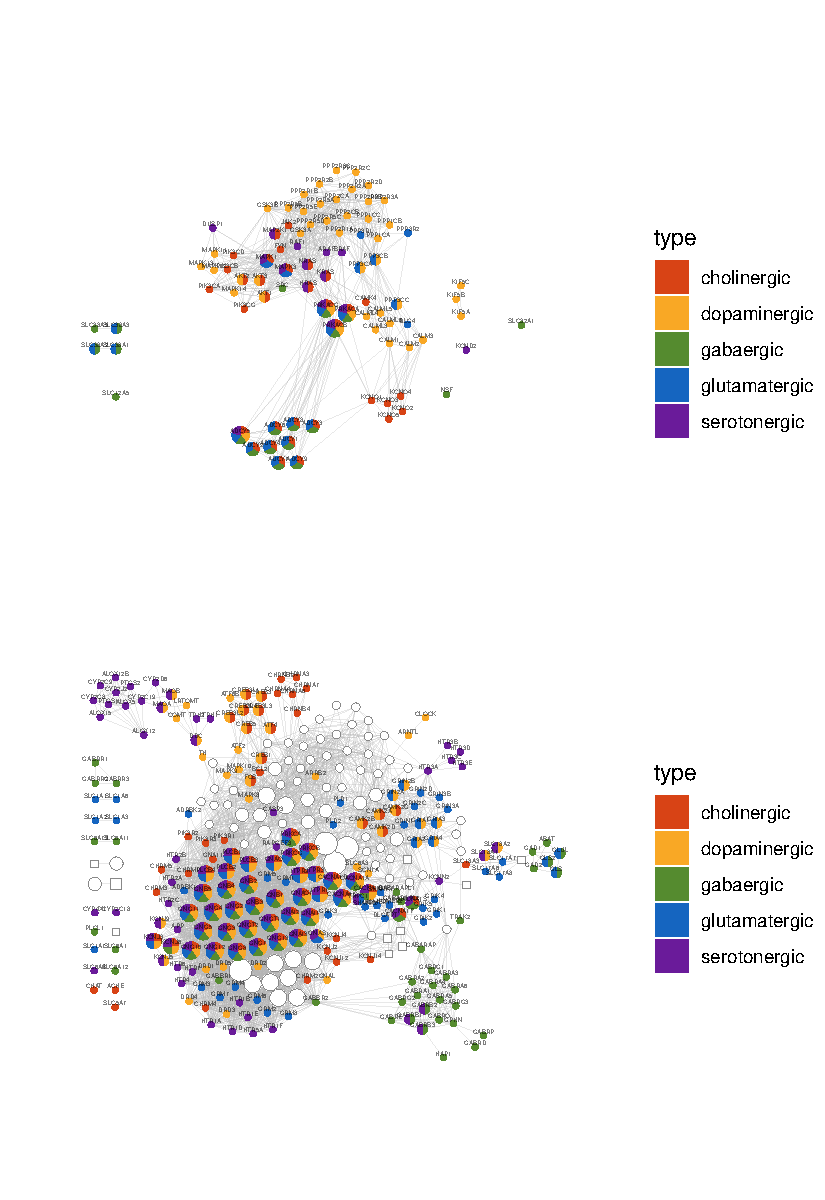
\includegraphics[width=\textwidth,height=0.9\textheight]{figs/analysis.network.fig3_raw-1}
\caption{test.}
\end{figure}

\clearpage

Additionally, we cumulatively count nodes by their categories (function
and neuroexclusivity) and inferred root:

\begin{Shaded}
\begin{Highlighting}[]
\NormalTok{cumulative_emergence <-}\StringTok{ }\NormalTok{vertices }\OperatorTok
\StringTok{  }\KeywordTok{select}\NormalTok{(root, annotation, }\DataTypeTok{is_neuroexclusive =}\NormalTok{ ne) }\OperatorTok
\StringTok{  }\CommentTok{# Adding clade info}
\StringTok{  }\KeywordTok{right_join}\NormalTok{(clade_names) }\OperatorTok
\StringTok{  }\CommentTok{# Pivoting from wide to long}
\StringTok{  }\KeywordTok{pivot_longer}\NormalTok{(annotation}\OperatorTok{:}\NormalTok{is_neuroexclusive, }\DataTypeTok{values_ptypes =} \KeywordTok{list}\NormalTok{(}\DataTypeTok{value =} \StringTok{"character"}\NormalTok{)) }\OperatorTok
\StringTok{  }\CommentTok{# Counting nodes by category (name) for each root}
\StringTok{  }\KeywordTok{count}\NormalTok{(root, clade_name, name, value) }\OperatorTok
\StringTok{  }\CommentTok{# Making absent counts explicit}
\StringTok{  }\KeywordTok{group_by}\NormalTok{(name) }\OperatorTok
\StringTok{  }\KeywordTok{complete}\NormalTok{(}\KeywordTok{nesting}\NormalTok{(root, clade_name), name, value, }\DataTypeTok{fill =} \KeywordTok{list}\NormalTok{(}\DataTypeTok{n =} \DecValTok{0}\NormalTok{)) }\OperatorTok
\StringTok{  }\CommentTok{# No reason to include NA observations in cumulative sum}
\StringTok{  }\NormalTok{na.omit }\OperatorTok
\StringTok{  }\CommentTok{# Cumulative sum node count at each root}
\StringTok{  }\KeywordTok{group_by}\NormalTok{(name, value) }\OperatorTok
\StringTok{  }\KeywordTok{mutate}\NormalTok{(}\DataTypeTok{cumulative_count =} \KeywordTok{order_by}\NormalTok{(}\OperatorTok{-}\NormalTok{root, }\KeywordTok{cumsum}\NormalTok{(n)))}
\end{Highlighting}
\end{Shaded}

Plotting such cumulative counts:

\begin{Shaded}
\begin{Highlighting}[]
\NormalTok{cumulative_emergence }\OperatorTok\StringTok{ }\NormalTok{ungroup }\OperatorTok
\StringTok{  }\CommentTok{# Creating ordered factors for plotting}
\StringTok{  }\KeywordTok{mutate}\NormalTok{(}
     \DataTypeTok{clade_name =} \KeywordTok{fct_reorder}\NormalTok{(clade_name, }\OperatorTok{-}\NormalTok{root)}
\NormalTok{    ,}\DataTypeTok{value      =} \KeywordTok{fct_reorder}\NormalTok{(value, name)}
\NormalTok{  )}

\KeywordTok{ggplot}\NormalTok{(cumulative_emergence) }\OperatorTok{+}
\StringTok{  }\CommentTok{#----- Barplot ------}
\StringTok{  }\KeywordTok{geom_bar}\NormalTok{(}
     \DataTypeTok{mapping     =} \KeywordTok{aes}\NormalTok{(clade_name, cumulative_count, }\DataTypeTok{group =}\NormalTok{ value)}
\NormalTok{    ,}\DataTypeTok{stat        =} \StringTok{"sum"}
\NormalTok{    ,}\DataTypeTok{fill        =} \StringTok{"#999999"}
\NormalTok{    ,}\DataTypeTok{show.legend =}\NormalTok{ F}
\NormalTok{  ) }\OperatorTok{+}
\StringTok{  }\CommentTok{#----- Lines ------}
\StringTok{  }\KeywordTok{geom_line}\NormalTok{(}
     \DataTypeTok{mapping =} \KeywordTok{aes}\NormalTok{(clade_name, cumulative_count, }\DataTypeTok{group =}\NormalTok{ value, }\DataTypeTok{color =}\NormalTok{ value)}
\NormalTok{    ,}\DataTypeTok{size    =} \DecValTok{1}
\NormalTok{  ) }\OperatorTok{+}
\StringTok{  }\CommentTok{#----- Styling ------}
\StringTok{  }\KeywordTok{scale_color_manual}\NormalTok{(}\DataTypeTok{values =}\NormalTok{ color_mappings) }\OperatorTok{+}
\StringTok{  }\KeywordTok{facet_grid}\NormalTok{(name }\OperatorTok{~}\StringTok{ }\NormalTok{.) }\OperatorTok{+}
\StringTok{  }\KeywordTok{theme}\NormalTok{(}
     \DataTypeTok{axis.title  =} \KeywordTok{element_blank}\NormalTok{()}
\NormalTok{    ,}\DataTypeTok{axis.text.x =} \KeywordTok{element_text}\NormalTok{(}\DataTypeTok{angle =} \DecValTok{-45}\NormalTok{, }\DataTypeTok{vjust =} \DecValTok{0}\NormalTok{, }\DataTypeTok{hjust =} \DecValTok{0}\NormalTok{)}
\NormalTok{  )}
\end{Highlighting}
\end{Shaded}

\begin{figure}

{\centering 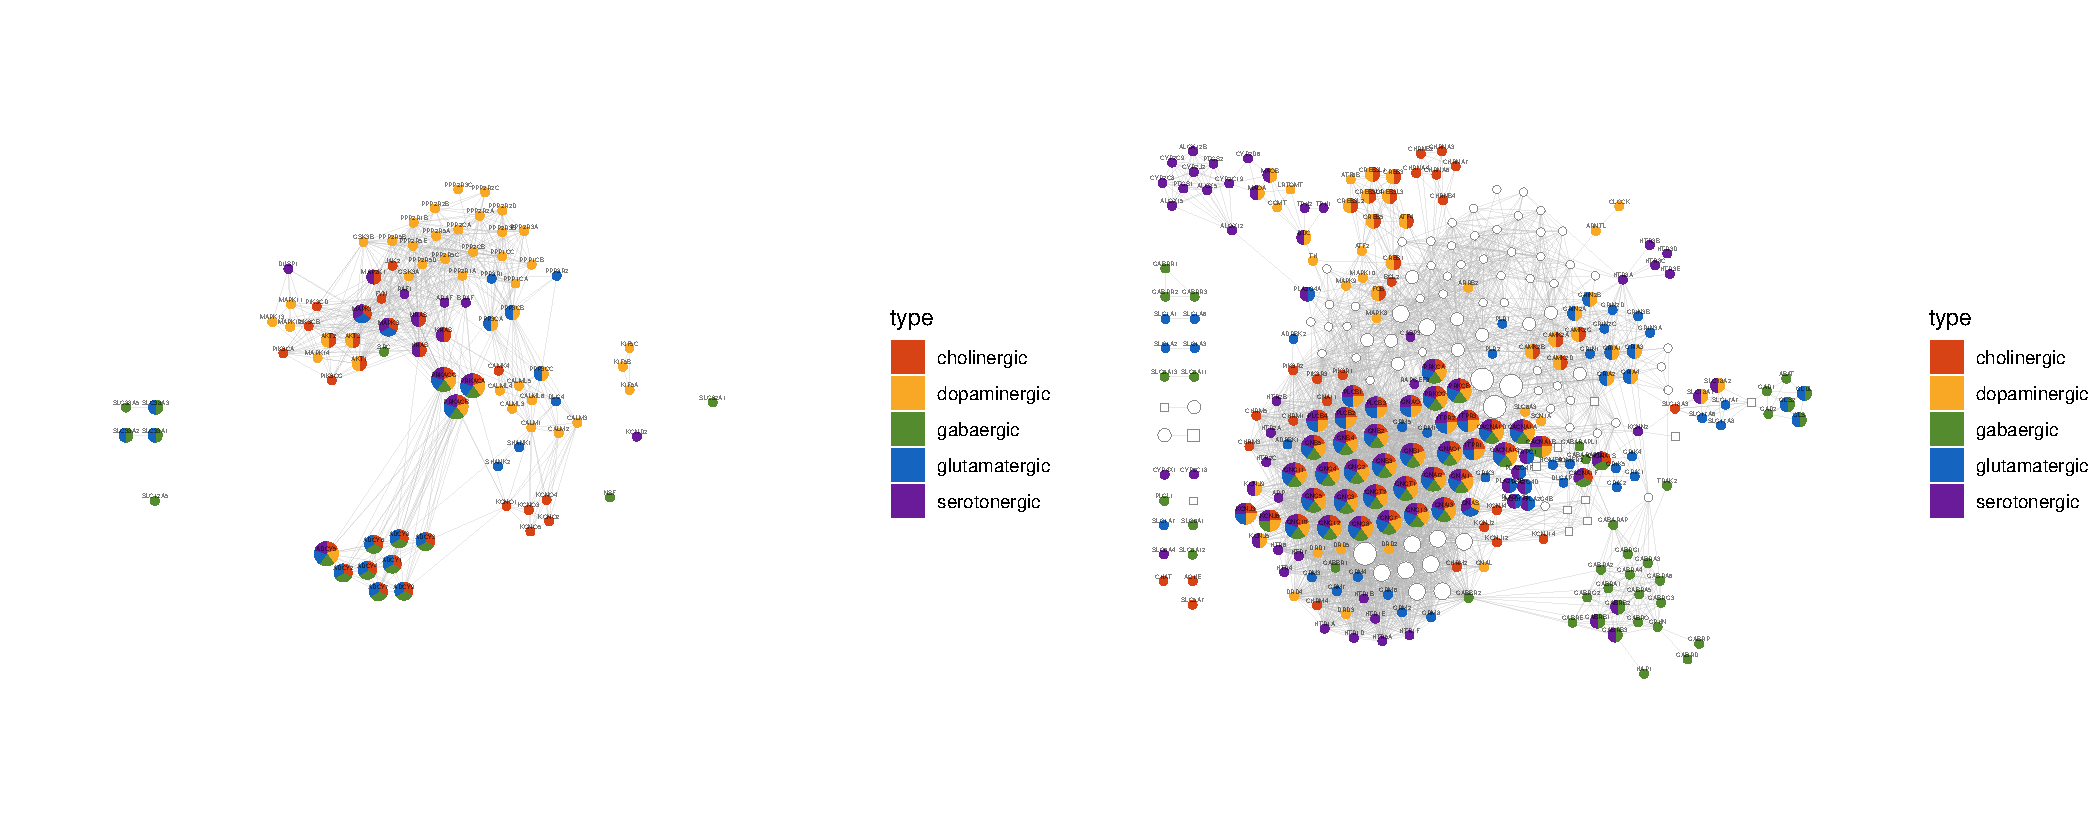
\includegraphics{figs/analysis.network.unnamed-chunk-11-1} 

}

\caption{Cumulative node counts by categories at each root.}\label{fig:unnamed-chunk-11}
\end{figure}

\hypertarget{manuscript-figure-4}{%
\subsubsection{Manuscript figure 4}\label{manuscript-figure-4}}

Visualizing nodes with roots \textless= 30 (Human-Porifera LCA) and
\textgreater= 26 (Human-Cnidaria LCA) at every distinct root.

\begin{Shaded}
\begin{Highlighting}[]
\NormalTok{plot_size <-}\StringTok{ }\KeywordTok{scale_radius}\NormalTok{(}\DataTypeTok{range =} \KeywordTok{c}\NormalTok{(}\FloatTok{0.5}\NormalTok{, }\FloatTok{1.5}\NormalTok{), }\DataTypeTok{guide =} \OtherTok{FALSE}\NormalTok{)}

\NormalTok{fig4 <-}\StringTok{ }\NormalTok{roots[roots }\OperatorTok{>=}\StringTok{ }\DecValTok{26} \OperatorTok{&}\StringTok{ }\NormalTok{roots }\OperatorTok{<=}\StringTok{ }\DecValTok{30}\NormalTok{] }\OperatorTok
\StringTok{  }\KeywordTok{imap}\NormalTok{(}\OperatorTok{~}\StringTok{ }\NormalTok{\{}
  \CommentTok{# Finding which genes should be drawn}
\NormalTok{  current_genes <-}\StringTok{ }\NormalTok{vertices }\OperatorTok\StringTok{ }\KeywordTok{filter}\NormalTok{(root }\OperatorTok{==}\StringTok{ }\NormalTok{.x)}
\NormalTok{  past_genes    <-}\StringTok{ }\NormalTok{vertices }\OperatorTok\StringTok{ }\KeywordTok{filter}\NormalTok{(root  }\OperatorTok{>}\StringTok{ }\NormalTok{.x)}
  
  \CommentTok{# Finding which edges should be drawn}
\NormalTok{  partial_ids   <-}\StringTok{ }\KeywordTok{c}\NormalTok{(current_genes[[}\StringTok{"string_id"}\NormalTok{]], past_genes[[}\StringTok{"string_id"}\NormalTok{]])}
\NormalTok{  which_edges   <-}\StringTok{ }\KeywordTok{apply}\NormalTok{(string_edgelist, }\DecValTok{1}\NormalTok{, }\ControlFlowTok{function}\NormalTok{(r) }\KeywordTok{all}\NormalTok{(r }\OperatorTok\StringTok{ }\NormalTok{partial_ids))}
\NormalTok{  partial_edges <-}\StringTok{ }\NormalTok{edges[which_edges }\OperatorTok\StringTok{ }\KeywordTok{rep}\NormalTok{(}\DecValTok{2}\NormalTok{),]}
  
\NormalTok{  plot_edges <-}\StringTok{ }\KeywordTok{geom_path}\NormalTok{(}
     \DataTypeTok{data    =}\NormalTok{ partial_edges}
\NormalTok{    ,}\DataTypeTok{mapping =}\NormalTok{ edge_aes}
\NormalTok{    ,}\DataTypeTok{color   =}\NormalTok{ edge_color}
\NormalTok{    ,}\DataTypeTok{size    =} \FloatTok{0.1}
\NormalTok{  )}
  
\NormalTok{  plot_past <-}\StringTok{ }\KeywordTok{geom_point}\NormalTok{(}
     \DataTypeTok{data    =}\NormalTok{ past_genes}
\NormalTok{    ,}\DataTypeTok{mapping =} \KeywordTok{aes}\NormalTok{(x, y, }\DataTypeTok{size =}\NormalTok{ size)}
\NormalTok{    ,}\DataTypeTok{fill    =}\NormalTok{ past_fill}
\NormalTok{    ,}\DataTypeTok{color   =}\NormalTok{ past_color}
\NormalTok{    ,}\DataTypeTok{shape   =}\NormalTok{ past_genes}\OperatorTok{$}\NormalTok{shape}
\NormalTok{    ,}\DataTypeTok{stroke  =} \FloatTok{0.25}
\NormalTok{  )}
  
\NormalTok{  plot_text <-}\StringTok{ }\KeywordTok{geom_text}\NormalTok{(}
     \DataTypeTok{data    =}\NormalTok{ current_genes}
\NormalTok{    ,}\DataTypeTok{mapping =}\NormalTok{ text_aes}
\NormalTok{    ,}\DataTypeTok{size    =} \FloatTok{0.8}
\NormalTok{    ,}\DataTypeTok{vjust   =} \FloatTok{-0.5}
\NormalTok{    ,}\DataTypeTok{nudge_y =} \DecValTok{1}
\NormalTok{    ,}\DataTypeTok{alpha   =} \FloatTok{0.5}
\NormalTok{  )}
  
\NormalTok{  plot_current_nodes <-}\StringTok{ }\KeywordTok{geom_point}\NormalTok{(}
     \DataTypeTok{data    =}\NormalTok{ current_genes}
\NormalTok{    ,}\DataTypeTok{mapping =} \KeywordTok{aes}\NormalTok{(x, y, }\DataTypeTok{fill =}\NormalTok{ annotation, }\DataTypeTok{size =}\NormalTok{ size)}
\NormalTok{    ,}\DataTypeTok{color   =}\NormalTok{ current_genes}\OperatorTok{$}\NormalTok{color_node}
\NormalTok{    ,}\DataTypeTok{shape   =}\NormalTok{ current_genes}\OperatorTok{$}\NormalTok{shape}
\NormalTok{    ,}\DataTypeTok{stroke  =} \FloatTok{0.25}
\NormalTok{  )}
  
\NormalTok{  remove_legend <-}\StringTok{ }\KeywordTok{guides}\NormalTok{(}\DataTypeTok{fill =} \StringTok{"none"}\NormalTok{, }\DataTypeTok{colour =} \StringTok{"none"}\NormalTok{)}
  
  \CommentTok{# Assembling}
  \KeywordTok{ggplot}\NormalTok{() }\OperatorTok{+}
\StringTok{    }\KeywordTok{ggtitle}\NormalTok{(}\KeywordTok{paste}\NormalTok{(.y, }\StringTok{"LCA"}\NormalTok{)) }\OperatorTok{+}
\StringTok{    }\NormalTok{diff_theme }\OperatorTok{+}
\StringTok{    }\NormalTok{xy_lim }\OperatorTok{+}
\StringTok{    }\NormalTok{plot_edges }\OperatorTok{+}
\StringTok{    }\NormalTok{plot_past }\OperatorTok{+}
\StringTok{    }\NormalTok{plot_current_nodes }\OperatorTok{+}
\StringTok{    }\NormalTok{plot_scales }\OperatorTok{+}
\StringTok{    }\NormalTok{plot_size }\OperatorTok{+}
\StringTok{    }\NormalTok{plot_text }\OperatorTok{+}
\StringTok{    }\NormalTok{remove_legend}
\NormalTok{\})}

\NormalTok{fig4 <-}\StringTok{ }\KeywordTok{invoke}\NormalTok{(grid.arrange, fig4, }\DataTypeTok{ncol =} \DecValTok{5}\NormalTok{)}
\end{Highlighting}
\end{Shaded}

\begin{Shaded}
\begin{Highlighting}[]
\CommentTok{# ggsave(}
\CommentTok{#   "plots/fig4_raw.pdf"}
\CommentTok{#   ,plot        = fig4}
\CommentTok{#   ,width       = 9*0.9}
\CommentTok{#   ,height      = 5*0.9}
\CommentTok{#   ,onefile     = F}
\CommentTok{#   ,useDingbats = F}
\CommentTok{# )}
\end{Highlighting}
\end{Shaded}

\clearpage

\begin{figure}
\centering
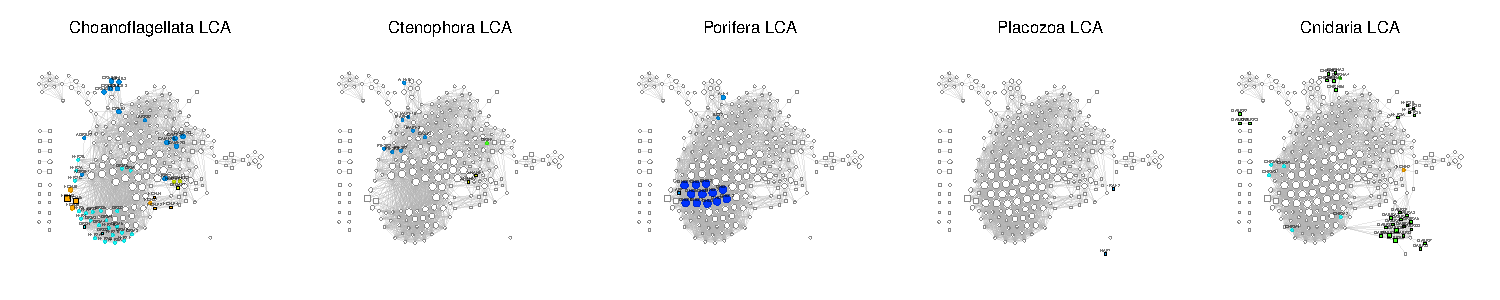
\includegraphics[width=1\textwidth,height=\textheight]{figs/analysis.network.fig4_raw-1}
\caption{test.}
\end{figure}

\clearpage

\hypertarget{supplementary-network-figures}{%
\subsubsection{Supplementary network
figures}\label{supplementary-network-figures}}

The following supplementary figures help us see what nodes have been
rooted at each LCA. Nodes rooted at previous LCAs are colored white.

\begin{Shaded}
\begin{Highlighting}[]
\NormalTok{system_plots   <-}\StringTok{ }\KeywordTok{list}\NormalTok{()}
\NormalTok{function_plots <-}\StringTok{ }\KeywordTok{list}\NormalTok{()}

\KeywordTok{iwalk}\NormalTok{(roots, }\OperatorTok{~}\StringTok{ }\NormalTok{\{}
  \CommentTok{# Finding which genes should be drawn}
\NormalTok{  current_genes <-}\StringTok{ }\NormalTok{vertices }\OperatorTok\StringTok{ }\KeywordTok{filter}\NormalTok{(root }\OperatorTok{==}\StringTok{ }\NormalTok{.x)}
\NormalTok{  past_genes    <-}\StringTok{ }\NormalTok{vertices }\OperatorTok\StringTok{ }\KeywordTok{filter}\NormalTok{(root  }\OperatorTok{>}\StringTok{ }\NormalTok{.x)}
  
  \CommentTok{# Finding which edges should be drawn}
\NormalTok{  partial_ids   <-}\StringTok{ }\KeywordTok{c}\NormalTok{(current_genes[[}\StringTok{"string_id"}\NormalTok{]], past_genes[[}\StringTok{"string_id"}\NormalTok{]])}
\NormalTok{  which_edges   <-}\StringTok{ }\KeywordTok{apply}\NormalTok{(string_edgelist, }\DecValTok{1}\NormalTok{, }\ControlFlowTok{function}\NormalTok{(r) }\KeywordTok{all}\NormalTok{(r }\OperatorTok\StringTok{ }\NormalTok{partial_ids))}
\NormalTok{  partial_edges <-}\StringTok{ }\NormalTok{edges[which_edges }\OperatorTok\StringTok{ }\KeywordTok{rep}\NormalTok{(}\DecValTok{2}\NormalTok{),]}
  
  \CommentTok{# Common elements -----------}
\NormalTok{  plot_edges <-}\StringTok{ }\KeywordTok{geom_path}\NormalTok{(}
     \DataTypeTok{data    =}\NormalTok{ partial_edges}
\NormalTok{    ,}\DataTypeTok{mapping =}\NormalTok{ edge_aes}
\NormalTok{    ,}\DataTypeTok{color   =}\NormalTok{ edge_color}
\NormalTok{    ,}\DataTypeTok{size    =} \FloatTok{0.1}
\NormalTok{  )}
  
\NormalTok{  plot_past <-}\StringTok{ }\KeywordTok{geom_point}\NormalTok{(}
     \DataTypeTok{data    =}\NormalTok{ past_genes}
\NormalTok{    ,}\DataTypeTok{mapping =} \KeywordTok{aes}\NormalTok{(x, y, }\DataTypeTok{size =}\NormalTok{ size)}
\NormalTok{    ,}\DataTypeTok{fill    =}\NormalTok{ past_fill}
\NormalTok{    ,}\DataTypeTok{color   =}\NormalTok{ past_color}
\NormalTok{    ,}\DataTypeTok{shape   =}\NormalTok{ past_genes}\OperatorTok{$}\NormalTok{shape}
\NormalTok{    ,}\DataTypeTok{stroke  =} \FloatTok{0.25}
\NormalTok{  )}
  
\NormalTok{  plot_text <-}\StringTok{ }\KeywordTok{geom_text}\NormalTok{(}\DataTypeTok{data =}\NormalTok{ current_genes, text_aes, }\DataTypeTok{size =} \FloatTok{0.75}\NormalTok{, }\DataTypeTok{nudge_y =} \DecValTok{4}\NormalTok{, }\DataTypeTok{alpha =} \FloatTok{0.5}\NormalTok{)}
  
\NormalTok{  base <-}\StringTok{ }\KeywordTok{ggplot}\NormalTok{() }\OperatorTok{+}
\StringTok{    }\KeywordTok{ggtitle}\NormalTok{(}\KeywordTok{paste0}\NormalTok{(}\StringTok{"Human-"}\NormalTok{, .y, }\StringTok{" LCA (#"}\NormalTok{, .x, }\StringTok{")"}\NormalTok{)) }\OperatorTok{+}
\StringTok{    }\NormalTok{diff_theme }\OperatorTok{+}
\StringTok{    }\NormalTok{xy_lim }\OperatorTok{+}
\StringTok{    }\NormalTok{plot_edges }\OperatorTok{+}
\StringTok{    }\NormalTok{plot_past }\OperatorTok{+}
\StringTok{    }\NormalTok{plot_size}
  
  \CommentTok{# Nodes colored by system -----------}
\NormalTok{  plot_current_pies <-}\StringTok{ }\KeywordTok{geom_scatterpie}\NormalTok{(}\DataTypeTok{data =}\NormalTok{ current_genes, pie_aes, }\DataTypeTok{cols =}\NormalTok{ systems, }\DataTypeTok{color =} \OtherTok{NA}\NormalTok{)}
  
\NormalTok{  system_plots[[}\KeywordTok{as.character}\NormalTok{(.x)]] <<-}\StringTok{ }\NormalTok{base }\OperatorTok{+}
\StringTok{    }\NormalTok{plot_current_pies }\OperatorTok{+}
\StringTok{    }\NormalTok{node_fill_scale }\OperatorTok{+}
\StringTok{    }\NormalTok{plot_text}
  
  \CommentTok{# Nodes colored by function --------}
\NormalTok{  plot_current_nodes <-}\StringTok{ }\KeywordTok{geom_point}\NormalTok{(}
     \DataTypeTok{data    =}\NormalTok{ current_genes}
\NormalTok{    ,}\DataTypeTok{mapping =} \KeywordTok{aes}\NormalTok{(x, y, }\DataTypeTok{fill =}\NormalTok{ annotation, }\DataTypeTok{size =}\NormalTok{ size)}
\NormalTok{    ,}\DataTypeTok{color   =}\NormalTok{ current_genes}\OperatorTok{$}\NormalTok{color_node}
\NormalTok{    ,}\DataTypeTok{shape   =}\NormalTok{ current_genes}\OperatorTok{$}\NormalTok{shape}
\NormalTok{    ,}\DataTypeTok{stroke  =} \FloatTok{0.25}
\NormalTok{  )}
  
\NormalTok{  function_plots[[}\KeywordTok{as.character}\NormalTok{(.x)]] <<-}\StringTok{ }\NormalTok{base }\OperatorTok{+}
\StringTok{    }\NormalTok{plot_current_nodes }\OperatorTok{+}
\StringTok{    }\NormalTok{plot_scales }\OperatorTok{+}
\StringTok{    }\NormalTok{plot_size }\OperatorTok{+}
\StringTok{    }\NormalTok{plot_text }\OperatorTok{+}
\StringTok{    }\KeywordTok{guides}\NormalTok{(}\DataTypeTok{fill =} \KeywordTok{guide_legend}\NormalTok{(}\DataTypeTok{override.aes =} \KeywordTok{list}\NormalTok{(}\DataTypeTok{shape =} \DecValTok{21}\NormalTok{))) }\CommentTok{# legend hack}
\NormalTok{\})}

\CommentTok{# Printing and saving}
\KeywordTok{arrangeGrob}\NormalTok{(}\DataTypeTok{grobs =}\NormalTok{ system_plots, }\DataTypeTok{ncol =} \DecValTok{2}\NormalTok{) }\OperatorTok\StringTok{ }\NormalTok{grid}\OperatorTok{::}\KeywordTok{grid.draw}\NormalTok{()}
\end{Highlighting}
\end{Shaded}

\clearpage

\thispagestyle{empty}

\pdfpageheight=22in

\begin{figure}[p]

\caption{caption.}\label{fig:analysis.network.fig_sup_systems-1}

{\centering 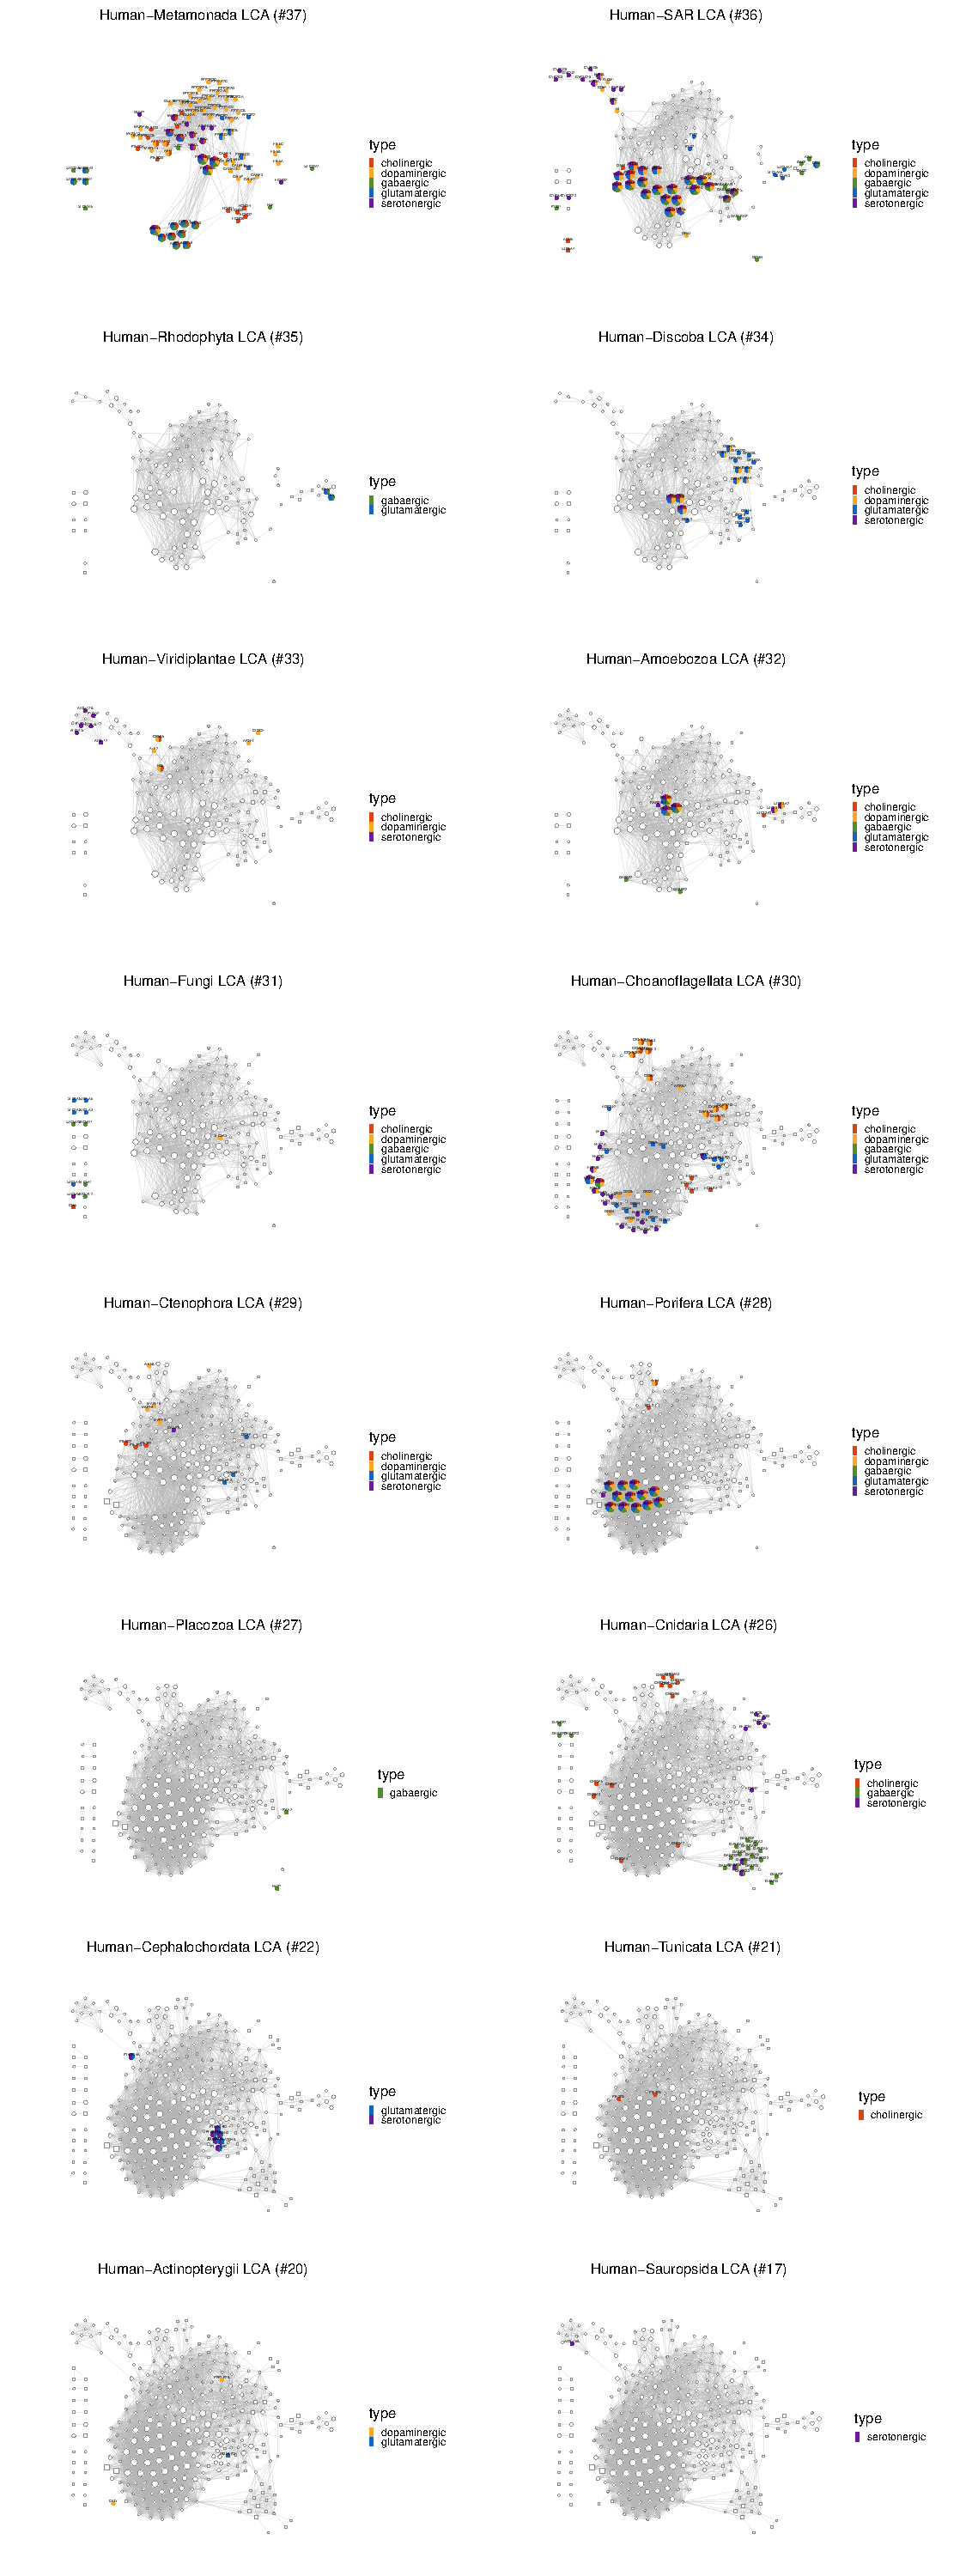
\includegraphics[width=7.5in, height=20in]{figs/analysis.network.fig_sup_systems-1} }

\end{figure}

\clearpage

\thispagestyle{empty}

\begin{Shaded}
\begin{Highlighting}[]
\KeywordTok{arrangeGrob}\NormalTok{(}\DataTypeTok{grobs =}\NormalTok{ function_plots, }\DataTypeTok{ncol =} \DecValTok{2}\NormalTok{) }\OperatorTok\StringTok{ }\NormalTok{grid}\OperatorTok{::}\KeywordTok{grid.draw}\NormalTok{()}
\end{Highlighting}
\end{Shaded}

\begin{figure}[p]

\caption{caption.}\label{fig:analysis.network.fig_sup_functions-1}

{\centering 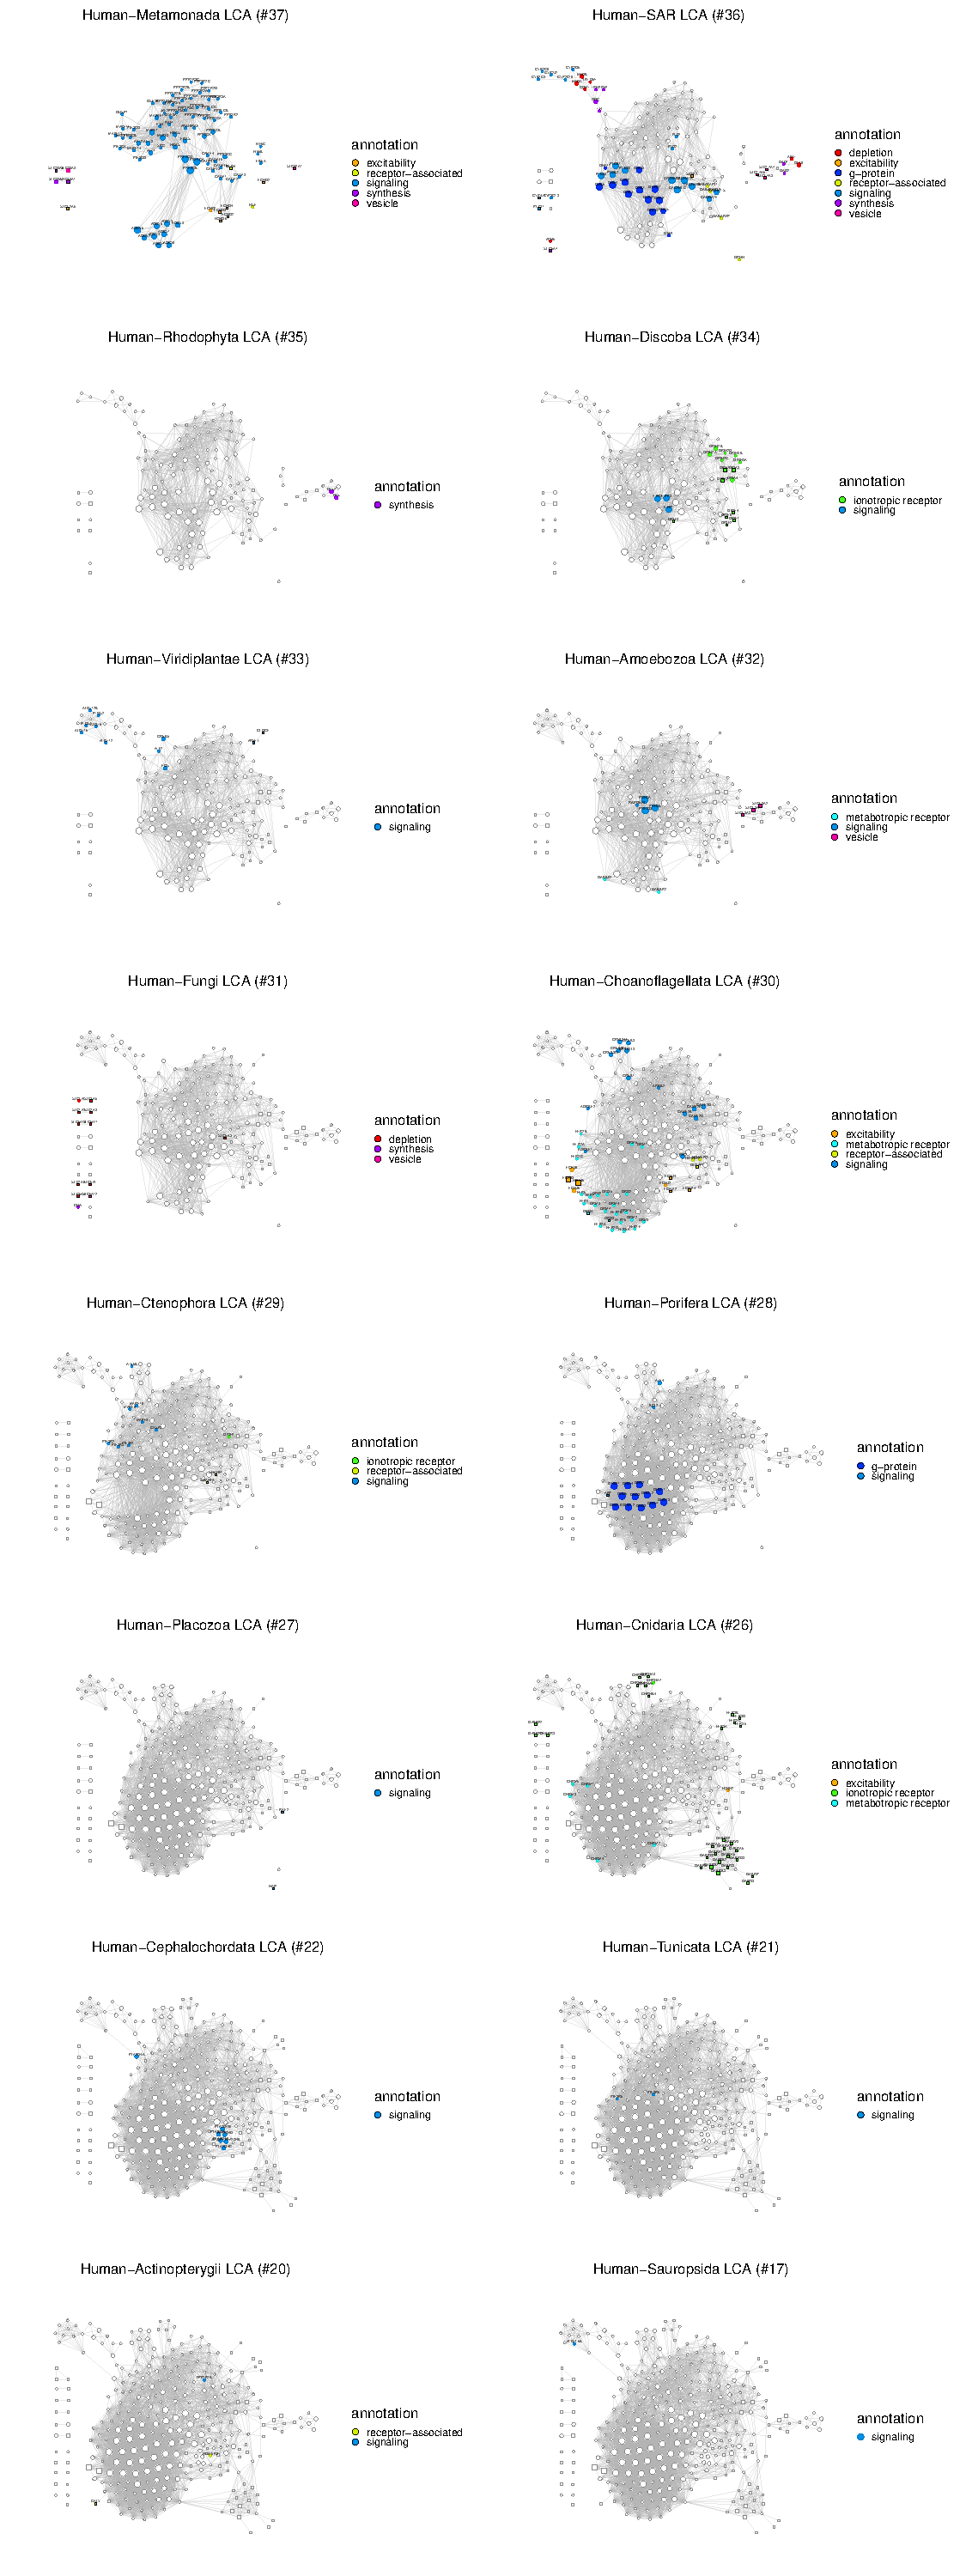
\includegraphics[width=7.5in, height=20in]{figs/analysis.network.fig_sup_functions-1} }

\end{figure}

\clearpage

\pdfpageheight=11in

\begin{Shaded}
\begin{Highlighting}[]
\CommentTok{# Pivoting vertices data.frame to enable faceting by systems}
\NormalTok{vertices_long <-}\StringTok{ }\KeywordTok{pivot_longer}\NormalTok{(}
   \DataTypeTok{data      =}\NormalTok{ vertices}
\NormalTok{  ,}\DataTypeTok{cols      =}\NormalTok{ systems}
\NormalTok{  ,}\DataTypeTok{names_to  =} \StringTok{"system"}
\NormalTok{  ,}\DataTypeTok{values_to =} \StringTok{"is_system"}
\NormalTok{) }\OperatorTok
\StringTok{  }\KeywordTok{mutate}\NormalTok{(}
     \DataTypeTok{system_color     =} \KeywordTok{ifelse}\NormalTok{(is_system,     system, }\StringTok{"other"}\NormalTok{)}
\NormalTok{    ,}\DataTypeTok{annotation_color =} \KeywordTok{ifelse}\NormalTok{(is_system, annotation, }\StringTok{"other"}\NormalTok{)}
\NormalTok{  )}

\NormalTok{edges_systems <-}\StringTok{ }\KeywordTok{inner_join}\NormalTok{(edges_long, vertices_long, }\DataTypeTok{by =} \StringTok{"string_id"}\NormalTok{)}

\CommentTok{# Determines from which root onwards and edge can be drawn (as well as its color)}
\NormalTok{edges_systems }\OperatorTok
\StringTok{  }\KeywordTok{group_by}\NormalTok{(group, system) }\OperatorTok
\StringTok{  }\KeywordTok{mutate}\NormalTok{(}
     \DataTypeTok{edge_system =} \KeywordTok{ifelse}\NormalTok{(is_system[}\KeywordTok{which.min}\NormalTok{(root)], system, }\StringTok{"other_edge"}\NormalTok{)}
\NormalTok{    ,}\DataTypeTok{edge_root   =} \KeywordTok{min}\NormalTok{(root)}
\NormalTok{  )}

\CommentTok{# Reference data.frame for inequality join}
\NormalTok{subsequent_duplicator <-}\StringTok{ }\NormalTok{vertices }\OperatorTok\StringTok{ }\KeywordTok{distinct}\NormalTok{(}\DataTypeTok{facet_root =}\NormalTok{ root)}

\CommentTok{# Simply duplicating emerging edges in subsequent roots}
\NormalTok{edges_in_roots <-}\StringTok{ }\NormalTok{edges_systems }\OperatorTok
\StringTok{  }\KeywordTok{fuzzy_inner_join}\NormalTok{(subsequent_duplicator, }\DataTypeTok{by =} \KeywordTok{c}\NormalTok{(}\StringTok{"edge_root"}\NormalTok{ =}\StringTok{ "facet_root"}\NormalTok{), }\DataTypeTok{match_fun =} \KeywordTok{list}\NormalTok{(}\StringTok{`}\DataTypeTok{>=}\StringTok{`}\NormalTok{)) }\OperatorTok
\StringTok{  }\KeywordTok{mutate}\NormalTok{(}
     \DataTypeTok{past =}\NormalTok{ edge_root }\OperatorTok{!=}\StringTok{ }\NormalTok{facet_root}
\NormalTok{    ,}\DataTypeTok{edge_color =} \KeywordTok{ifelse}\NormalTok{(}\OperatorTok{!}\NormalTok{past }\OperatorTok{&}\StringTok{ }\NormalTok{(system_color }\OperatorTok{==}\StringTok{ }\NormalTok{edge_system), system, }\StringTok{"other_edge"}\NormalTok{)}
\NormalTok{  )}

\CommentTok{# Simply duplicating emerging nodes in subsequent roots}
\NormalTok{nodes_in_roots <-}\StringTok{ }\NormalTok{vertices_long }\OperatorTok
\StringTok{  }\KeywordTok{fuzzy_inner_join}\NormalTok{(subsequent_duplicator, }\DataTypeTok{by =} \KeywordTok{c}\NormalTok{(}\StringTok{"root"}\NormalTok{ =}\StringTok{ "facet_root"}\NormalTok{), }\DataTypeTok{match_fun =} \KeywordTok{list}\NormalTok{(}\StringTok{`}\DataTypeTok{>=}\StringTok{`}\NormalTok{)) }\OperatorTok
\StringTok{  }\KeywordTok{mutate}\NormalTok{(}
     \DataTypeTok{past              =}\NormalTok{ root }\OperatorTok{!=}\StringTok{ }\NormalTok{facet_root}
\NormalTok{    ,}\DataTypeTok{system_color      =} \KeywordTok{ifelse}\NormalTok{(past, }\StringTok{"past"}\NormalTok{, system_color)}
\NormalTok{    ,}\DataTypeTok{system_border     =} \KeywordTok{ifelse}\NormalTok{(}\OperatorTok{!}\NormalTok{past }\OperatorTok{&}\StringTok{ }\NormalTok{ne, }\StringTok{"ne_border"}\NormalTok{, system_color)}
\NormalTok{    ,}\DataTypeTok{annotation_border =} \KeywordTok{ifelse}\NormalTok{(}\OperatorTok{!}\NormalTok{past }\OperatorTok{&}\StringTok{ }\NormalTok{ne, }\StringTok{"ne_border"}\NormalTok{, annotation_color)}
\NormalTok{  )}

\KeywordTok{ggplot}\NormalTok{() }\OperatorTok{+}
\StringTok{  }\KeywordTok{geom_path}\NormalTok{(}
     \DataTypeTok{data    =}\NormalTok{ edges_in_roots}
\NormalTok{    ,}\DataTypeTok{mapping =} \KeywordTok{aes}\NormalTok{(}
       \DataTypeTok{x     =}\NormalTok{ x}
\NormalTok{      ,}\DataTypeTok{y     =}\NormalTok{ y}
\NormalTok{      ,}\DataTypeTok{group =}\NormalTok{ group}
\NormalTok{    )}
\NormalTok{    ,}\DataTypeTok{color   =}\NormalTok{ color_mappings[edges_in_roots[[}\StringTok{"edge_color"}\NormalTok{]]] }\OperatorTok\StringTok{ }\KeywordTok{alpha}\NormalTok{(}\FloatTok{0.3}\NormalTok{)}
\NormalTok{    ,}\DataTypeTok{size    =} \FloatTok{0.1}
\NormalTok{  ) }\OperatorTok{+}
\StringTok{  }\KeywordTok{geom_point}\NormalTok{(}
     \DataTypeTok{data =}\NormalTok{ nodes_in_roots }
\NormalTok{    ,}\DataTypeTok{mapping =} \KeywordTok{aes}\NormalTok{(}
       \DataTypeTok{x     =}\NormalTok{ x}
\NormalTok{      ,}\DataTypeTok{y     =}\NormalTok{ y}
\NormalTok{      ,}\DataTypeTok{size  =}\NormalTok{ size}
\NormalTok{      ,}\DataTypeTok{shape =}\NormalTok{ shape}
\NormalTok{      ,}\DataTypeTok{fill  =}\NormalTok{ system_color}
\NormalTok{      ,}\DataTypeTok{color =}\NormalTok{ system_border}
\NormalTok{    )}
\NormalTok{  ) }\OperatorTok{+}
\StringTok{  }\NormalTok{node_fill_scale }\OperatorTok{+}
\StringTok{  }\NormalTok{node_color_scale }\OperatorTok{+}
\StringTok{  }\KeywordTok{scale_shape_identity}\NormalTok{() }\OperatorTok{+}
\StringTok{  }\KeywordTok{scale_radius}\NormalTok{(}\DataTypeTok{range =} \KeywordTok{c}\NormalTok{(}\DecValTok{1}\NormalTok{, }\DecValTok{3}\NormalTok{)) }\OperatorTok{+}
\StringTok{  }\KeywordTok{facet_grid}\NormalTok{(}\OperatorTok{-}\NormalTok{facet_root }\OperatorTok{~}\StringTok{ }\NormalTok{system, }\DataTypeTok{switch =} \StringTok{"y"}\NormalTok{) }\OperatorTok{+}
\StringTok{  }\KeywordTok{theme_void}\NormalTok{() }\OperatorTok{+}
\StringTok{  }\KeywordTok{theme}\NormalTok{(}
     \DataTypeTok{strip.text.y     =} \KeywordTok{element_text}\NormalTok{(}\DataTypeTok{angle =} \DecValTok{90}\NormalTok{)}
\NormalTok{    ,}\DataTypeTok{strip.background =} \KeywordTok{element_rect}\NormalTok{(}\DataTypeTok{color =} \StringTok{"#c0c0c0"}\NormalTok{, }\DataTypeTok{fill =} \StringTok{"#c0c0c0"}\NormalTok{, }\DataTypeTok{size =} \FloatTok{0.5}\NormalTok{, }\DataTypeTok{linetype =} \StringTok{"solid"}\NormalTok{)}
\NormalTok{    ,}\DataTypeTok{panel.border     =} \KeywordTok{element_rect}\NormalTok{(}\DataTypeTok{color =} \StringTok{"#c0c0c0"}\NormalTok{, }\DataTypeTok{fill =} \OtherTok{NA}\NormalTok{, }\DataTypeTok{size =} \FloatTok{0.5}\NormalTok{, }\DataTypeTok{linetype =} \StringTok{"solid"}\NormalTok{)}
\NormalTok{  ) }\OperatorTok{+}
\StringTok{  }\KeywordTok{guides}\NormalTok{(}\DataTypeTok{fill =} \StringTok{"none"}\NormalTok{, }\DataTypeTok{color =} \StringTok{"none"}\NormalTok{, }\DataTypeTok{size =} \StringTok{"none"}\NormalTok{)}
\end{Highlighting}
\end{Shaded}

\clearpage

\thispagestyle{empty}

\pdfpagewidth=16.6in \pdfpageheight=37.6in

\begin{figure}[p]

\caption{caption.}\label{fig:analysis.network.faceted_systems-1}

{\centering 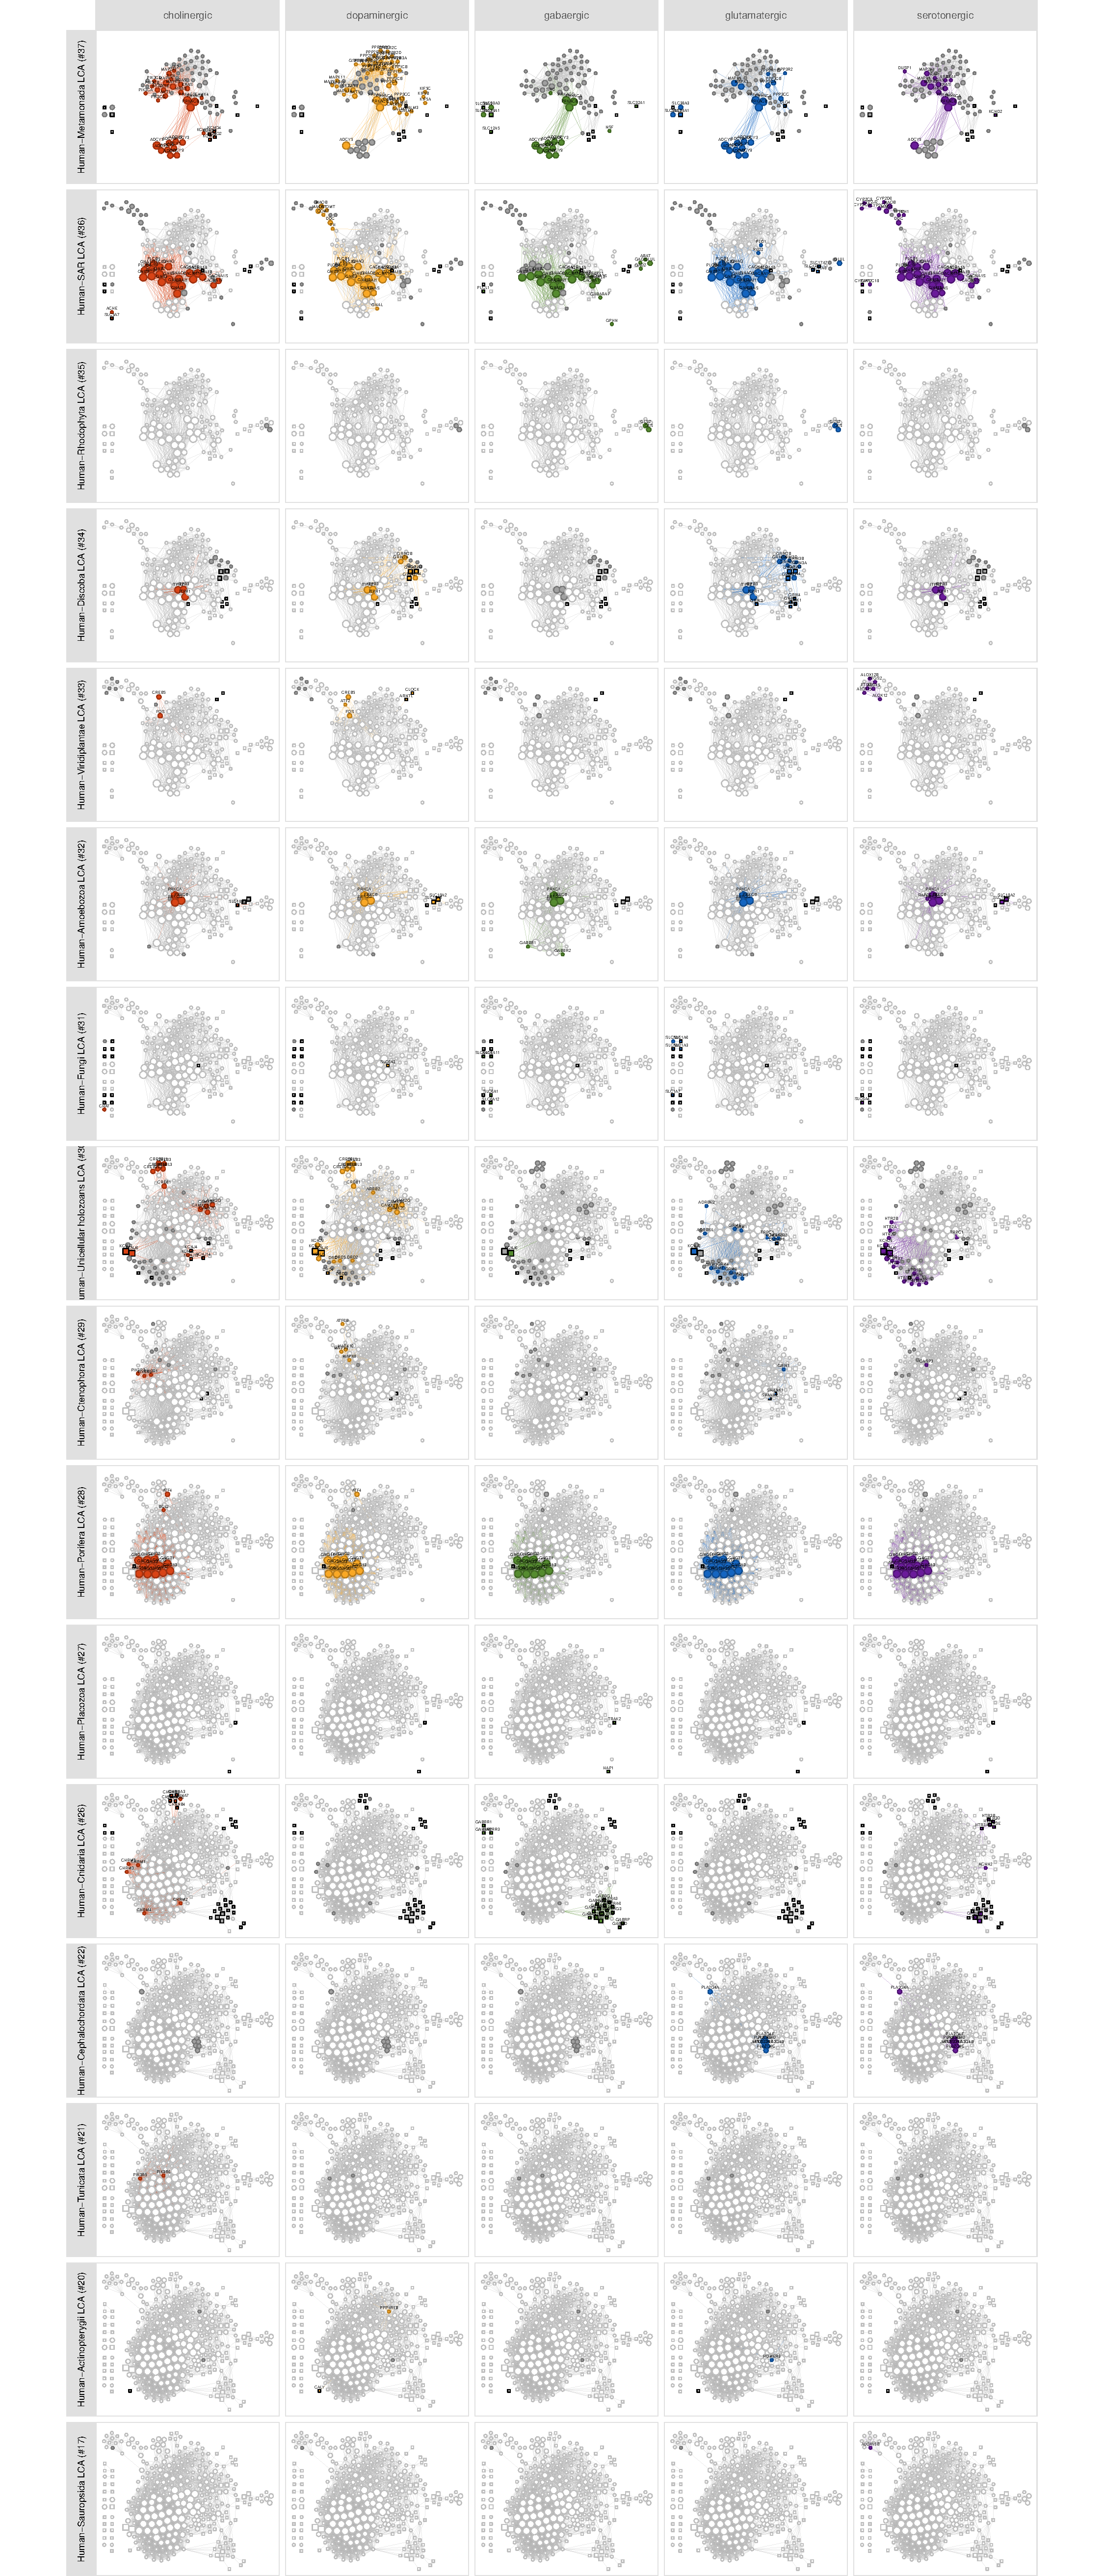
\includegraphics[height=35in, width=15in]{figs/analysis.network.faceted_systems-1} }

\end{figure}

\clearpage

\pdfpagewidth=8.5in \pdfpageheight=11in

\hypertarget{manuscript-set-diagrams}{%
\subsubsection{Manuscript set diagrams}\label{manuscript-set-diagrams}}

Given the dificulties of joining ggplot and base plots, the set diagrams
have to be plotted by themselves:

\begin{Shaded}
\begin{Highlighting}[]
\CommentTok{# We have to manually find the correct order of colors}
\CommentTok{# Because UpSetR does not understand named vectors}
\NormalTok{get_colors <-}\StringTok{ }\ControlFlowTok{function}\NormalTok{(df) \{}
\NormalTok{  ordered_systems <-}\StringTok{ }\NormalTok{df }\OperatorTok
\StringTok{    }\KeywordTok{select}\NormalTok{(systems) }\OperatorTok
\StringTok{    }\NormalTok{colSums }\OperatorTok
\StringTok{    }\KeywordTok{extract}\NormalTok{(. }\OperatorTok{>}\StringTok{ }\DecValTok{0}\NormalTok{) }\OperatorTok
\StringTok{    }\KeywordTok{extract}\NormalTok{(}\KeywordTok{order}\NormalTok{(., }\KeywordTok{names}\NormalTok{(.), }\DataTypeTok{decreasing =}\NormalTok{ T))}

\NormalTok{  color_mappings[}\KeywordTok{names}\NormalTok{(ordered_systems)]}
\NormalTok{\}}

\CommentTok{# Figure 1A set diagram}
\KeywordTok{upset}\NormalTok{(}
   \KeywordTok{select}\NormalTok{(vertices, systems)}
\NormalTok{  ,}\DataTypeTok{mb.ratio        =} \KeywordTok{c}\NormalTok{(}\FloatTok{0.7}\NormalTok{, }\FloatTok{0.3}\NormalTok{)}
\NormalTok{  ,}\DataTypeTok{order.by        =} \StringTok{"freq"}
\NormalTok{  ,}\DataTypeTok{mainbar.y.label =} \StringTok{"System Intersections"}
\NormalTok{  ,}\DataTypeTok{sets.x.label    =} \StringTok{"Genes per system"}
\NormalTok{  ,}\DataTypeTok{text.scale      =}\NormalTok{ upset_texts}
\NormalTok{  ,}\DataTypeTok{point.size      =} \FloatTok{3.5}
\NormalTok{  ,}\DataTypeTok{line.size       =} \DecValTok{1}
\NormalTok{  ,}\DataTypeTok{sets.bar.color  =} \KeywordTok{get_colors}\NormalTok{(vertices)}
\NormalTok{)}
\KeywordTok{dev.print}\NormalTok{(pdf, }\StringTok{"plots/fig1a_set_raw.pdf"}\NormalTok{, }\DataTypeTok{width =} \DecValTok{18}\NormalTok{, }\DataTypeTok{height =} \DecValTok{10}\NormalTok{, }\DataTypeTok{onefile =}\NormalTok{ F, }\DataTypeTok{useDingbats =}\NormalTok{ F)}

\CommentTok{# Figure 3A set diagram}
\NormalTok{fig3a_set <-}\StringTok{ }\NormalTok{vertices }\OperatorTok\StringTok{ }\KeywordTok{filter}\NormalTok{(root }\OperatorTok{==}\StringTok{ }\DecValTok{37}\NormalTok{) }\OperatorTok\StringTok{ }\KeywordTok{select}\NormalTok{(systems)}
\KeywordTok{upset}\NormalTok{(}
\NormalTok{   fig3a_set}
\NormalTok{  ,}\DataTypeTok{mb.ratio        =} \KeywordTok{c}\NormalTok{(}\FloatTok{0.7}\NormalTok{, }\FloatTok{0.3}\NormalTok{)}
\NormalTok{  ,}\DataTypeTok{order.by        =} \StringTok{"freq"}
\NormalTok{  ,}\DataTypeTok{mainbar.y.label =} \StringTok{"System Intersections"}
\NormalTok{  ,}\DataTypeTok{sets.x.label    =} \StringTok{"Genes per system"}
\NormalTok{  ,}\DataTypeTok{text.scale      =}\NormalTok{ upset_texts}
\NormalTok{  ,}\DataTypeTok{point.size      =} \FloatTok{3.5}
\NormalTok{  ,}\DataTypeTok{line.size       =} \DecValTok{1}
\NormalTok{  ,}\DataTypeTok{sets.bar.color  =} \KeywordTok{get_colors}\NormalTok{(fig3a_set)}
\NormalTok{)}
\KeywordTok{dev.print}\NormalTok{(pdf, }\StringTok{"plots/fig3a_set_raw.pdf"}\NormalTok{, }\DataTypeTok{width =} \DecValTok{16}\NormalTok{, }\DataTypeTok{height =} \DecValTok{8}\NormalTok{, }\DataTypeTok{onefile =}\NormalTok{ F, }\DataTypeTok{useDingbats =}\NormalTok{ F)}

\CommentTok{# Figure 3B set diagram}
\NormalTok{fig3b_set <-}\StringTok{ }\NormalTok{vertices }\OperatorTok\StringTok{ }\KeywordTok{filter}\NormalTok{(root }\OperatorTok{<}\StringTok{ }\DecValTok{37} \OperatorTok{&}\StringTok{ }\NormalTok{root }\OperatorTok{>=}\StringTok{ }\DecValTok{26}\NormalTok{) }\OperatorTok\StringTok{ }\KeywordTok{select}\NormalTok{(systems)}
\KeywordTok{upset}\NormalTok{(}
\NormalTok{   fig3b_set}
\NormalTok{  ,}\DataTypeTok{mb.ratio        =} \KeywordTok{c}\NormalTok{(}\FloatTok{0.7}\NormalTok{, }\FloatTok{0.3}\NormalTok{)}
\NormalTok{  ,}\DataTypeTok{order.by        =} \StringTok{"freq"}
\NormalTok{  ,}\DataTypeTok{mainbar.y.label =} \StringTok{"System Intersections"}
\NormalTok{  ,}\DataTypeTok{sets.x.label    =} \StringTok{"Genes per system"}
\NormalTok{  ,}\DataTypeTok{text.scale      =}\NormalTok{ upset_texts}
\NormalTok{  ,}\DataTypeTok{point.size      =} \FloatTok{3.5}
\NormalTok{  ,}\DataTypeTok{line.size       =} \DecValTok{1}
\NormalTok{  ,}\DataTypeTok{sets.bar.color  =} \KeywordTok{get_colors}\NormalTok{(fig3b_set)}
\NormalTok{)}
\KeywordTok{dev.print}\NormalTok{(pdf, }\StringTok{"plots/fig3b_set_raw.pdf"}\NormalTok{, }\DataTypeTok{width =} \DecValTok{16}\NormalTok{, }\DataTypeTok{height =} \DecValTok{8}\NormalTok{, }\DataTypeTok{onefile =}\NormalTok{ F, }\DataTypeTok{useDingbats =}\NormalTok{ F)}
\end{Highlighting}
\end{Shaded}

\begin{figure}
\subfloat[Set diagram for Figure 1A\label{fig:unnamed-chunk-121}]{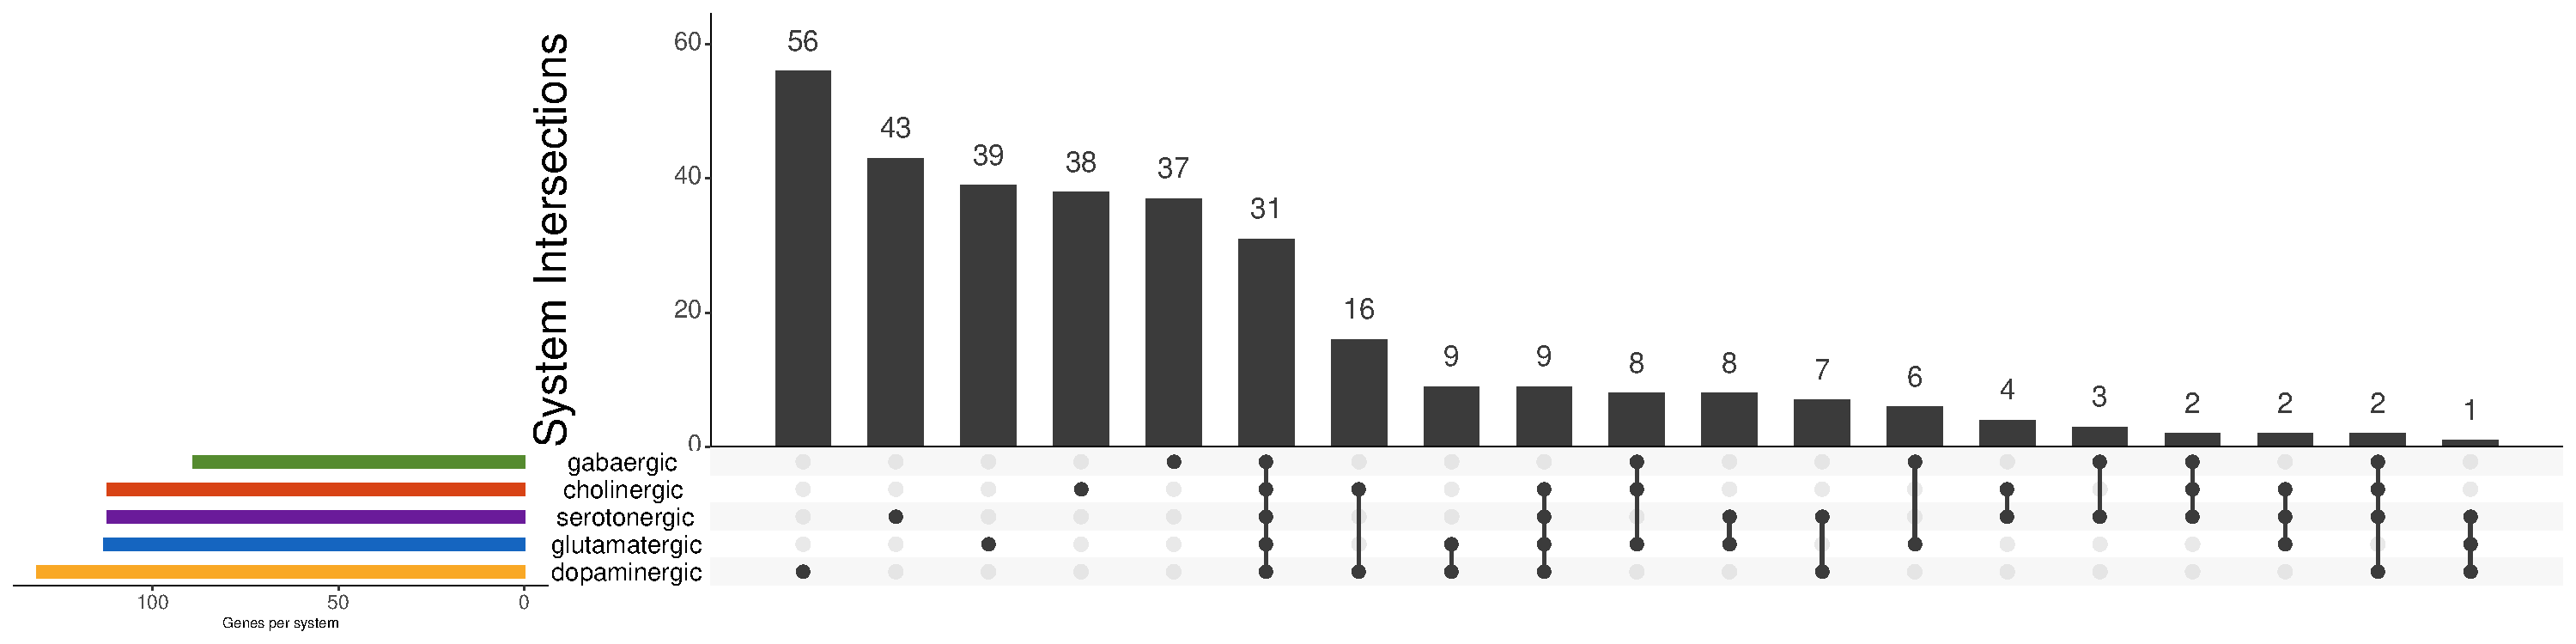
\includegraphics{figs/analysis.network.unnamed-chunk-12-1} }\newline\subfloat[Set diagram for Figure 3A\label{fig:unnamed-chunk-122}]{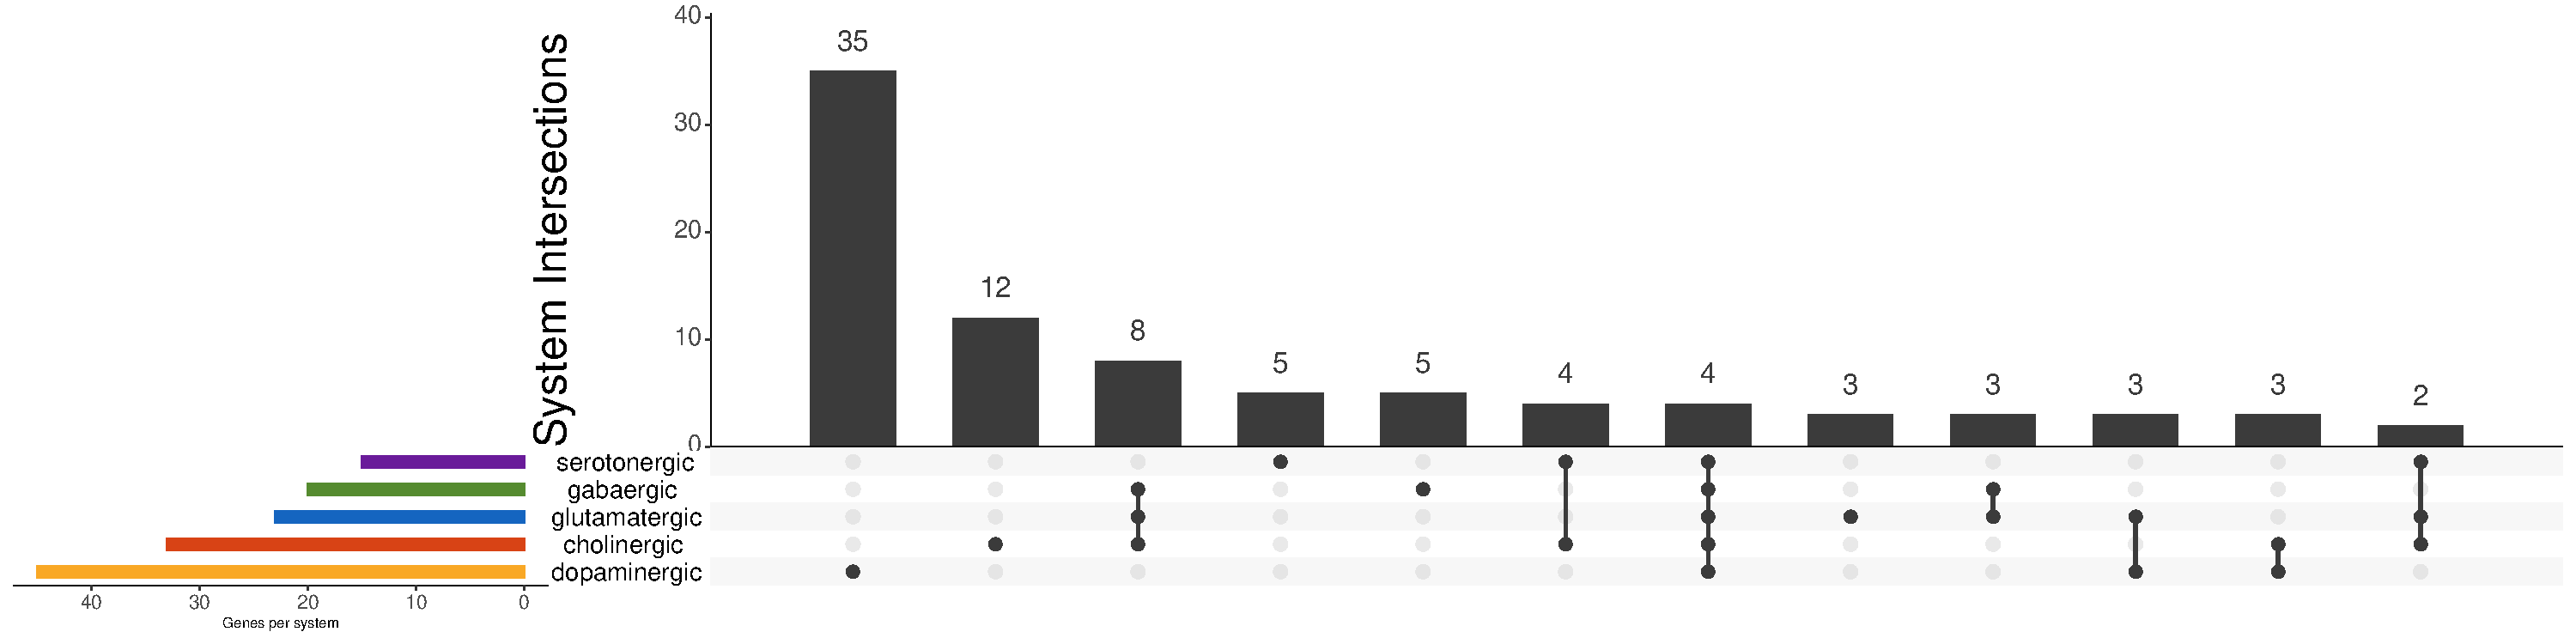
\includegraphics{figs/analysis.network.unnamed-chunk-12-2} }\newline\subfloat[Set diagram for Figure 3B\label{fig:unnamed-chunk-123}]{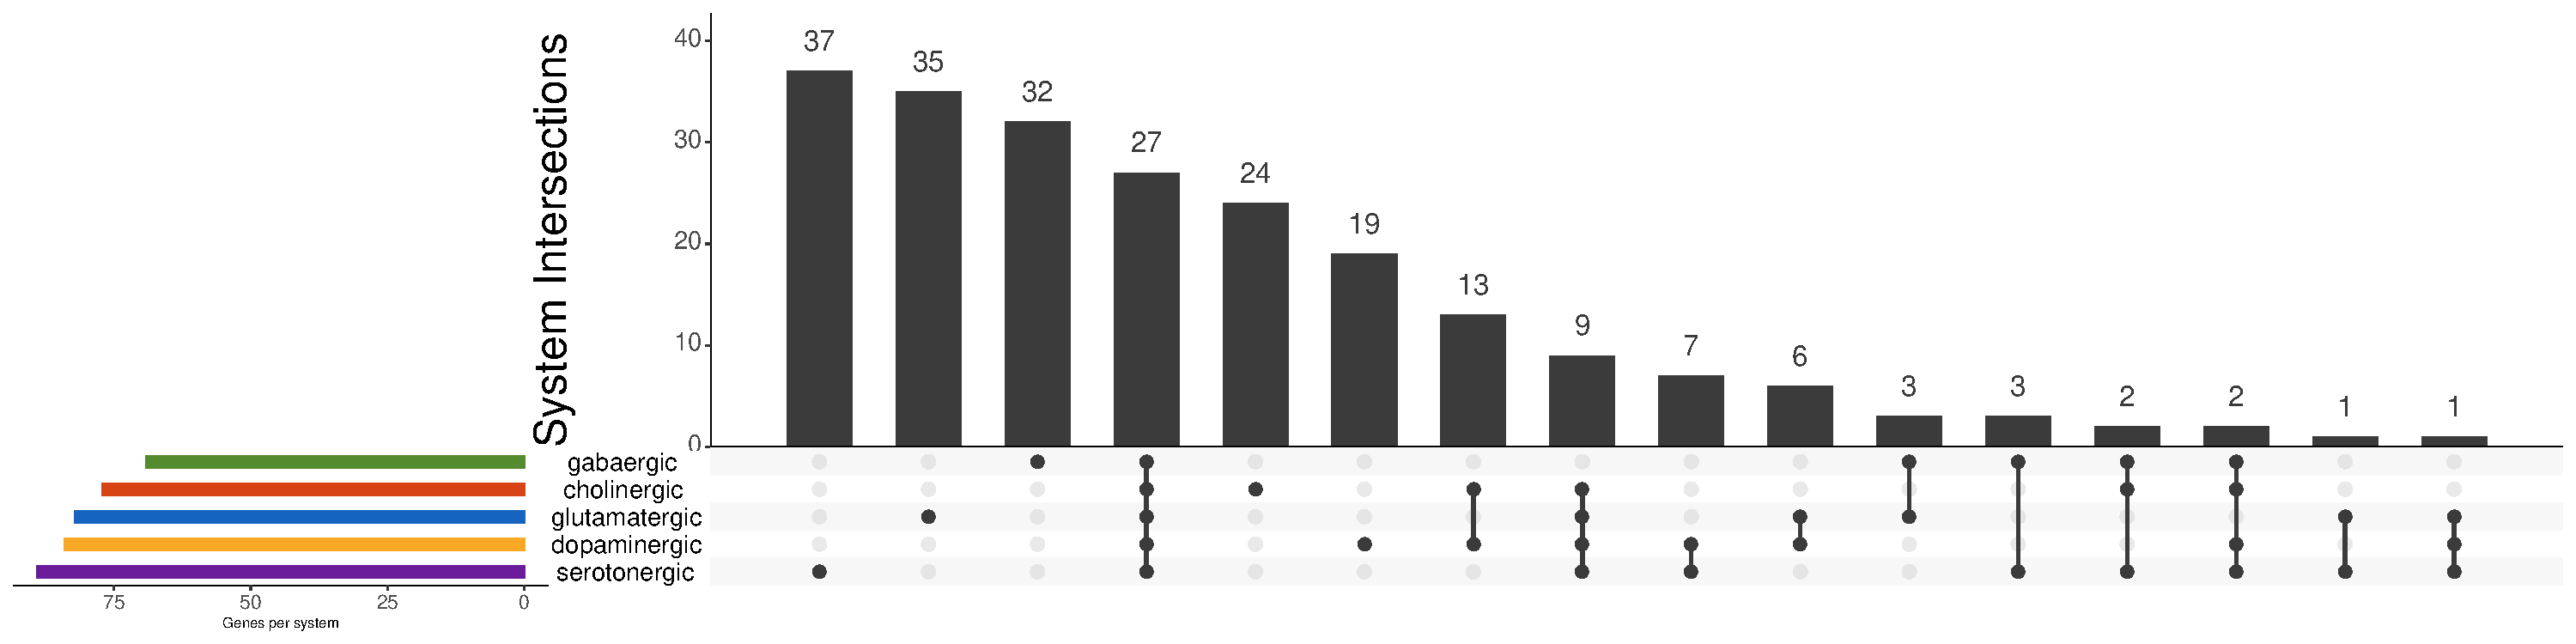
\includegraphics{figs/analysis.network.unnamed-chunk-12-3} }\caption{Set diagrams}\label{fig:unnamed-chunk-12}
\end{figure}


\hypertarget{abundance}{%
\subsection{Abundance}\label{abundance}}

A Loading initial resources:

\begin{Shaded}
\begin{Highlighting}[]
\CommentTok{# Data manipulation}
\KeywordTok{library}\NormalTok{(tidyverse)}
\KeywordTok{library}\NormalTok{(magrittr)}

\CommentTok{# Utils}
\KeywordTok{library}\NormalTok{(neurotransmissionevolution)}

\CommentTok{# Packaged data}
\KeywordTok{data}\NormalTok{(}
\NormalTok{   cogs}
\NormalTok{  ,gene_ids}
\NormalTok{  ,gene_cogs}
\NormalTok{  ,string_eukaryotes}
\NormalTok{  ,}\DataTypeTok{package =} \StringTok{"neurotransmissionevolution"}
\NormalTok{)}

\CommentTok{# Fresh analysis data}
\NormalTok{cog_roots                   <-}\StringTok{ }\KeywordTok{read_tsv}\NormalTok{(}\StringTok{"geneplast_roots.tsv"}\NormalTok{,             }\DataTypeTok{col_types =} \StringTok{"ci"}\NormalTok{)}
\NormalTok{clade_names                 <-}\StringTok{ }\KeywordTok{read_tsv}\NormalTok{(}\StringTok{"geneplast_clade_names.tsv"}\NormalTok{,       }\DataTypeTok{col_types =} \StringTok{"ic"}\NormalTok{)}
\NormalTok{clade_taxids                <-}\StringTok{ }\KeywordTok{read_tsv}\NormalTok{(}\StringTok{"geneplast_clade_taxids.tsv"}\NormalTok{,      }\DataTypeTok{col_types =} \StringTok{"ici"}\NormalTok{)}

\CommentTok{# Collapsing similar functions}
\NormalTok{gene_annotation <-}\StringTok{ }\KeywordTok{read_tsv}\NormalTok{(}\StringTok{"../data/gene_annotation.tsv"}\NormalTok{, }\DataTypeTok{col_types =} \StringTok{"cc"}\NormalTok{) }\OperatorTok
\StringTok{  }\KeywordTok{mutate}\NormalTok{(}\DataTypeTok{annotation =} \KeywordTok{case_when}\NormalTok{(}
     \KeywordTok{grepl}\NormalTok{(}\StringTok{"clearance"}\NormalTok{,   annotation) }\OperatorTok{~}\StringTok{ "depletion"}
\NormalTok{    ,}\KeywordTok{grepl}\NormalTok{(}\StringTok{"degradation"}\NormalTok{, annotation) }\OperatorTok{~}\StringTok{ "depletion"}
\NormalTok{    ,}\KeywordTok{grepl}\NormalTok{(}\StringTok{"transport"}\NormalTok{,   annotation) }\OperatorTok{~}\StringTok{ "synthesis"}
\NormalTok{    ,}\OtherTok{TRUE} \OperatorTok{~}\StringTok{ }\NormalTok{annotation}
\NormalTok{  ))}
\end{Highlighting}
\end{Shaded}

We start by setting up reusable data frames with useful metrics.

\begin{Shaded}
\begin{Highlighting}[]
\CommentTok{# If a gene has more than 1 COG, select the oldest one.}
\CommentTok{# This is unusual, but can happen in cases of gene fusion, for instance.}
\NormalTok{gene_cogs }\OperatorTok
\StringTok{  }\KeywordTok{inner_join}\NormalTok{(cog_roots) }\OperatorTok
\StringTok{  }\KeywordTok{group_by}\NormalTok{(string_id) }\OperatorTok
\StringTok{  }\KeywordTok{filter}\NormalTok{(root }\OperatorTok{==}\StringTok{ }\KeywordTok{max}\NormalTok{(root))}

\CommentTok{# The function of a COG is the function of its proteins}
\NormalTok{cog_annotation <-}\StringTok{ }\NormalTok{gene_ids }\OperatorTok
\StringTok{  }\KeywordTok{inner_join}\NormalTok{(gene_cogs) }\OperatorTok
\StringTok{  }\KeywordTok{inner_join}\NormalTok{(gene_annotation) }\OperatorTok
\StringTok{  }\KeywordTok{distinct}\NormalTok{(cog_id, annotation)}

\CommentTok{# Number of proteins in a COG in every species}
\NormalTok{cog_abundance_by_taxid <-}\StringTok{ }\NormalTok{cogs }\OperatorTok
\StringTok{  }\KeywordTok{filter}\NormalTok{(cog_id }\OperatorTok\StringTok{ }\NormalTok{gene_cogs[[}\StringTok{"cog_id"}\NormalTok{]]) }\OperatorTok
\StringTok{  }\KeywordTok{count}\NormalTok{(taxid, cog_id,  }\DataTypeTok{name =} \StringTok{"abundance"}\NormalTok{) }\OperatorTok
\StringTok{  }\KeywordTok{left_join}\NormalTok{(cog_annotation)}

\CommentTok{# Mapping species to clade info}
\NormalTok{ordered_species <-}\StringTok{ }\NormalTok{string_eukaryotes }\OperatorTok
\StringTok{  }\KeywordTok{select}\NormalTok{(taxid, ncbi_name) }\OperatorTok
\StringTok{  }\KeywordTok{left_join}\NormalTok{(clade_taxids) }\OperatorTok
\StringTok{  }\KeywordTok{left_join}\NormalTok{(clade_names, }\DataTypeTok{by =} \KeywordTok{c}\NormalTok{(}\StringTok{"lca"}\NormalTok{ =}\StringTok{ "root"}\NormalTok{)) }\OperatorTok
\StringTok{  }\KeywordTok{mutate}\NormalTok{(}
     \DataTypeTok{ncbi_name  =} \KeywordTok{fct_reorder}\NormalTok{(ncbi_name, }\OperatorTok{-}\NormalTok{taxid_order)}
\NormalTok{    ,}\DataTypeTok{clade_name =} \KeywordTok{fct_reorder}\NormalTok{(clade_name, }\OperatorTok{-}\NormalTok{taxid_order)}
\NormalTok{  )}

\CommentTok{# Plotting colors}
\NormalTok{annotation_colors <-}\StringTok{ }\KeywordTok{c}\NormalTok{(}
   \StringTok{"depletion"}\NormalTok{             =}\StringTok{ "#F40000"}
\NormalTok{  ,}\StringTok{"excitability"}\NormalTok{          =}\StringTok{ "#FFAB00"}
\NormalTok{  ,}\StringTok{"receptor-associated"}\NormalTok{   =}\StringTok{ "#D6EE00"}
\NormalTok{  ,}\StringTok{"ionotropic receptor"}\NormalTok{   =}\StringTok{ "#43FF1C"}
\NormalTok{  ,}\StringTok{"metabotropic receptor"}\NormalTok{ =}\StringTok{ "#18FFFF"}
\NormalTok{  ,}\StringTok{"signaling"}\NormalTok{             =}\StringTok{ "#0091EA"}
\NormalTok{  ,}\StringTok{"g-protein"}\NormalTok{             =}\StringTok{ "#0033ff"}
\NormalTok{  ,}\StringTok{"synthesis"}\NormalTok{             =}\StringTok{ "#AA00FF"}
\NormalTok{  ,}\StringTok{"vesicle"}\NormalTok{               =}\StringTok{ "#FF00AA"}
\NormalTok{)}
\end{Highlighting}
\end{Shaded}

The average orthogroup abundances are finally computed for each species
according to the function of orthogroups.

\begin{Shaded}
\begin{Highlighting}[]
\NormalTok{avg_abundance_by_function <-}\StringTok{ }\NormalTok{cog_abundance_by_taxid }\OperatorTok
\StringTok{  }\KeywordTok{group_by}\NormalTok{(taxid, annotation) }\OperatorTok
\StringTok{  }\KeywordTok{summarise}\NormalTok{(}\DataTypeTok{avg_abundance =} \KeywordTok{mean}\NormalTok{(abundance)) }\OperatorTok
\StringTok{  }\CommentTok{# Adding species and clade info}
\StringTok{  }\KeywordTok{left_join}\NormalTok{(ordered_species)}
\end{Highlighting}
\end{Shaded}

Plotting:

\begin{Shaded}
\begin{Highlighting}[]
\CommentTok{# This vertical line indicates the first metazoan (Mnemiopsis leidyi / Ctenophora)}
\NormalTok{metazoa_line <-}\StringTok{ }\KeywordTok{geom_vline}\NormalTok{(}
   \DataTypeTok{xintercept =} \StringTok{"Mnemiopsis leidyi"}
\NormalTok{  ,}\DataTypeTok{color      =} \StringTok{"#FF0000"}
\NormalTok{  ,}\DataTypeTok{linetype   =} \StringTok{"11"}
\NormalTok{  ,}\DataTypeTok{alpha      =} \DecValTok{1}
\NormalTok{  ,}\DataTypeTok{size       =} \FloatTok{0.25}
\NormalTok{)}
\NormalTok{tick_function <-}\StringTok{ }\ControlFlowTok{function}\NormalTok{(x) \{}
  \KeywordTok{seq}\NormalTok{(x[}\DecValTok{2}\NormalTok{], }\DecValTok{0}\NormalTok{, }\DataTypeTok{length.out =} \DecValTok{3}\NormalTok{) }\OperatorTok\StringTok{ }\KeywordTok{head}\NormalTok{(}\OperatorTok{-}\DecValTok{1}\NormalTok{) }\OperatorTok\StringTok{ }\KeywordTok{tail}\NormalTok{(}\OperatorTok{-}\DecValTok{1}\NormalTok{) }\OperatorTok\StringTok{ }\NormalTok{\{ }\KeywordTok{ceiling}\NormalTok{(.}\OperatorTok{/}\DecValTok{5}\NormalTok{)}\OperatorTok{*}\DecValTok{5}\NormalTok{ \}}
\NormalTok{\}}

\CommentTok{# Capping abundance values based on metazoan mean}
\NormalTok{capped_abundance_by_function <-}\StringTok{ }\NormalTok{avg_abundance_by_function }\OperatorTok
\StringTok{  }\CommentTok{# mutate(capped_abundance = ifelse(abundance >= 100, 100, abundance)) %>%}
\StringTok{  }\KeywordTok{group_by}\NormalTok{(annotation) }\OperatorTok
\StringTok{  }\KeywordTok{mutate}\NormalTok{(}
     \DataTypeTok{max_abundance =}\NormalTok{ avg_abundance[lca }\OperatorTok{<=}\StringTok{ }\DecValTok{29}\NormalTok{] }\OperatorTok\StringTok{ }\NormalTok{\{ }\KeywordTok{mean}\NormalTok{(.) }\OperatorTok{+}\StringTok{ }\DecValTok{3}\OperatorTok{*}\KeywordTok{sd}\NormalTok{(.) \}}
\NormalTok{    ,}\DataTypeTok{avg_abundance =} \KeywordTok{ifelse}\NormalTok{(avg_abundance }\OperatorTok{>=}\StringTok{ }\NormalTok{max_abundance, }\KeywordTok{pmin}\NormalTok{(max_abundance, }\DecValTok{100}\NormalTok{), }\KeywordTok{pmin}\NormalTok{(avg_abundance, }\DecValTok{100}\NormalTok{))}
\NormalTok{  )}

\CommentTok{# Plotting}
\NormalTok{abundance_plot <-}\StringTok{ }\KeywordTok{ggplot}\NormalTok{(capped_abundance_by_function) }\OperatorTok{+}
\StringTok{  }\CommentTok{# Geoms  ----------------}
\StringTok{  }\NormalTok{metazoa_line }\OperatorTok{+}
\StringTok{  }\KeywordTok{geom_bar}\NormalTok{(}
     \KeywordTok{aes}\NormalTok{(}\DataTypeTok{x =}\NormalTok{ ncbi_name, }\DataTypeTok{y =}\NormalTok{ avg_abundance, }\DataTypeTok{fill =}\NormalTok{ annotation, }\DataTypeTok{color =} \KeywordTok{after_scale}\NormalTok{(}\KeywordTok{darken}\NormalTok{(fill, }\FloatTok{0.1}\NormalTok{)))}
\NormalTok{    ,}\DataTypeTok{stat =} \StringTok{"identity"}
\NormalTok{  ) }\OperatorTok{+}
\StringTok{  }\CommentTok{# Labels  ---------------}
\StringTok{  }\KeywordTok{xlab}\NormalTok{(}\StringTok{"Taxa"}\NormalTok{) }\OperatorTok{+}
\StringTok{  }\KeywordTok{ylab}\NormalTok{(}\StringTok{"Average protein abundance in orthologous groups"}\NormalTok{) }\OperatorTok{+}
\StringTok{  }\CommentTok{# Scales ----------------}
\StringTok{  }\KeywordTok{scale_y_continuous}\NormalTok{(}\DataTypeTok{breaks =}\NormalTok{ tick_function, }\DataTypeTok{minor_breaks =} \OtherTok{NULL}\NormalTok{) }\OperatorTok{+}
\StringTok{  }\KeywordTok{scale_fill_manual}\NormalTok{(}\DataTypeTok{values =}\NormalTok{ annotation_colors }\OperatorTok\StringTok{ }\KeywordTok{darken}\NormalTok{(}\FloatTok{0.1}\NormalTok{)) }\OperatorTok{+}
\StringTok{  }\CommentTok{# Styling ---------------}
\StringTok{  }\KeywordTok{facet_grid}\NormalTok{(annotation }\OperatorTok{~}\StringTok{ }\NormalTok{clade_name, }\DataTypeTok{scales =} \StringTok{"free"}\NormalTok{, }\DataTypeTok{space =} \StringTok{"free"}\NormalTok{) }\OperatorTok{+}
\StringTok{  }\KeywordTok{theme}\NormalTok{(}
     \DataTypeTok{panel.spacing      =} \KeywordTok{unit}\NormalTok{(}\FloatTok{2.5}\NormalTok{, }\StringTok{"pt"}\NormalTok{)}
\NormalTok{    ,}\DataTypeTok{strip.background.x =} \KeywordTok{element_blank}\NormalTok{()}
\NormalTok{    ,}\DataTypeTok{strip.background.y =} \KeywordTok{element_rect}\NormalTok{(}\DataTypeTok{fill=}\StringTok{"#E0E0E0"}\NormalTok{)}
\NormalTok{    ,}\DataTypeTok{panel.grid.major.x =} \KeywordTok{element_blank}\NormalTok{()}
\NormalTok{    ,}\DataTypeTok{panel.grid.major.y =} \KeywordTok{element_line}\NormalTok{(}\DataTypeTok{colour =} \StringTok{"#F5F5F5"}\NormalTok{, }\DataTypeTok{size =} \FloatTok{0.25}\NormalTok{)}
\NormalTok{    ,}\DataTypeTok{panel.background   =} \KeywordTok{element_rect}\NormalTok{(}\DataTypeTok{fill =} \StringTok{'#EEEEEE'}\NormalTok{, }\DataTypeTok{colour =} \StringTok{'#E0E0E0'}\NormalTok{)}
\NormalTok{    ,}\DataTypeTok{strip.text.x       =} \KeywordTok{element_text}\NormalTok{(}\DataTypeTok{size =} \DecValTok{6}\NormalTok{, }\DataTypeTok{angle =} \DecValTok{90}\NormalTok{, }\DataTypeTok{hjust =} \DecValTok{0}\NormalTok{, }\DataTypeTok{vjust =} \FloatTok{0.5}\NormalTok{)}
\NormalTok{    ,}\DataTypeTok{strip.text.y       =} \KeywordTok{element_text}\NormalTok{(}\DataTypeTok{size =} \DecValTok{8}\NormalTok{, }\DataTypeTok{vjust =} \FloatTok{0.5}\NormalTok{)}
\NormalTok{    ,}\DataTypeTok{axis.text.x        =} \KeywordTok{element_text}\NormalTok{(}\DataTypeTok{size =} \DecValTok{2}\NormalTok{, }\DataTypeTok{angle =} \DecValTok{-45}\NormalTok{, }\DataTypeTok{vjust =} \DecValTok{0}\NormalTok{, }\DataTypeTok{hjust =} \DecValTok{0}\NormalTok{)}
\NormalTok{    ,}\DataTypeTok{axis.text.y        =} \KeywordTok{element_text}\NormalTok{(}\DataTypeTok{size =} \DecValTok{6}\NormalTok{)}
\NormalTok{    ,}\DataTypeTok{legend.position    =} \StringTok{"none"}
\NormalTok{  )}
\KeywordTok{ggsave}\NormalTok{(}\StringTok{"plots/fig5_raw.pdf"}\NormalTok{, abundance_plot, }\DataTypeTok{width =} \DecValTok{16}\NormalTok{, }\DataTypeTok{height =} \DecValTok{6}\NormalTok{)}

\CommentTok{# Uncapped abundances for supplementary text}
\NormalTok{abundance_plot }\OperatorTok\StringTok{ }\NormalTok{avg_abundance_by_function}
\end{Highlighting}
\end{Shaded}

\begin{figure}

{\centering 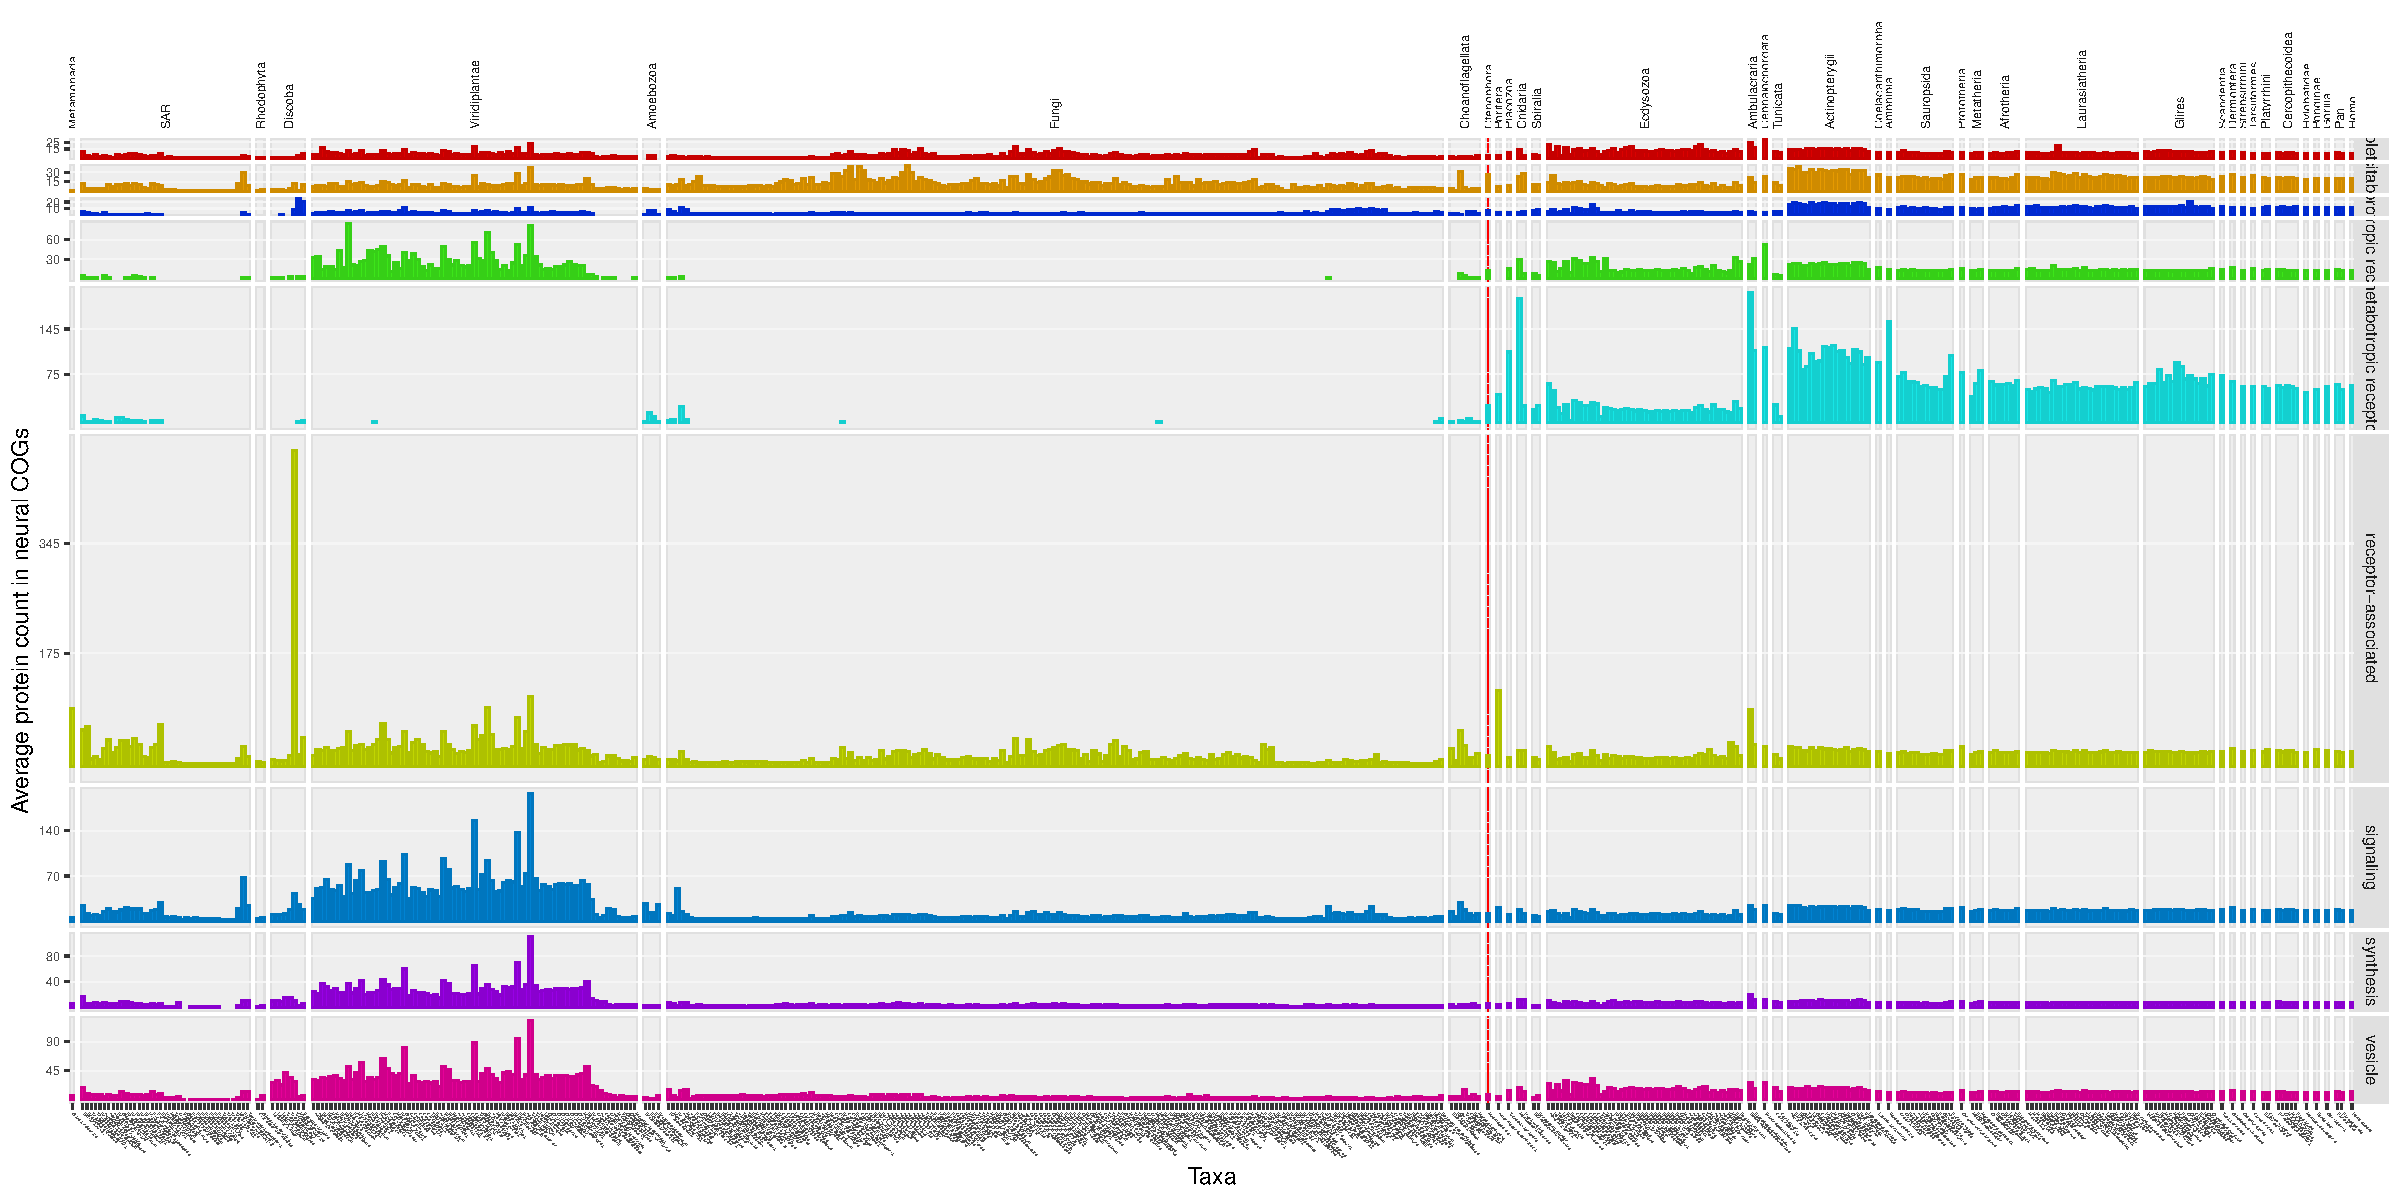
\includegraphics{figs/analysis.abundance.unnamed-chunk-5-1} 

}

\caption{Abundance values by species. Species are ordered like in Supplementary Figure 1.}\label{fig:unnamed-chunk-5}
\end{figure}

Species-specific average abundances, now averaged by clades:

\begin{Shaded}
\begin{Highlighting}[]
\KeywordTok{ggplot}\NormalTok{(avg_abundance_by_function) }\OperatorTok{+}
\StringTok{  }\KeywordTok{geom_bar}\NormalTok{(}
    \KeywordTok{aes}\NormalTok{(}\DataTypeTok{x =}\NormalTok{ clade_name, }\DataTypeTok{y =}\NormalTok{ avg_abundance, }\DataTypeTok{fill =}\NormalTok{ annotation, }\DataTypeTok{color =} \KeywordTok{after_scale}\NormalTok{(}\KeywordTok{darken}\NormalTok{(fill, }\FloatTok{0.1}\NormalTok{)))}
\NormalTok{    ,}\DataTypeTok{stat =} \StringTok{"summary"}
\NormalTok{    ,}\DataTypeTok{fun  =} \StringTok{"mean"}
\NormalTok{  ) }\OperatorTok{+}
\StringTok{  }\KeywordTok{scale_y_continuous}\NormalTok{(}\DataTypeTok{breaks =}\NormalTok{ tick_function, }\DataTypeTok{minor_breaks =} \OtherTok{NULL}\NormalTok{) }\OperatorTok{+}
\StringTok{  }\KeywordTok{scale_fill_manual}\NormalTok{(}\DataTypeTok{values =}\NormalTok{ annotation_colors, }\DataTypeTok{guide =} \StringTok{"none"}\NormalTok{) }\OperatorTok{+}
\StringTok{  }\KeywordTok{facet_grid}\NormalTok{(annotation }\OperatorTok{~}\StringTok{ }\NormalTok{., }\DataTypeTok{scales =} \StringTok{"free"}\NormalTok{, }\DataTypeTok{space =} \StringTok{"free_y"}\NormalTok{) }\OperatorTok{+}
\StringTok{  }\KeywordTok{theme}\NormalTok{(}
     \DataTypeTok{panel.spacing      =} \KeywordTok{unit}\NormalTok{(}\DecValTok{1}\NormalTok{, }\StringTok{"pt"}\NormalTok{)}
\NormalTok{    ,}\DataTypeTok{strip.text.y       =} \KeywordTok{element_text}\NormalTok{(}\DataTypeTok{angle =} \DecValTok{0}\NormalTok{, }\DataTypeTok{hjust =} \DecValTok{0}\NormalTok{)}
\NormalTok{    ,}\DataTypeTok{axis.text.x        =} \KeywordTok{element_text}\NormalTok{(}\DataTypeTok{size =} \DecValTok{5}\NormalTok{, }\DataTypeTok{angle =} \DecValTok{-45}\NormalTok{, }\DataTypeTok{vjust =} \DecValTok{0}\NormalTok{, }\DataTypeTok{hjust =} \DecValTok{0}\NormalTok{)}
\NormalTok{    ,}\DataTypeTok{axis.text.y        =} \KeywordTok{element_text}\NormalTok{(}\DataTypeTok{size =} \DecValTok{5}\NormalTok{)}
\NormalTok{  )}
\end{Highlighting}
\end{Shaded}

\begin{figure}

{\centering 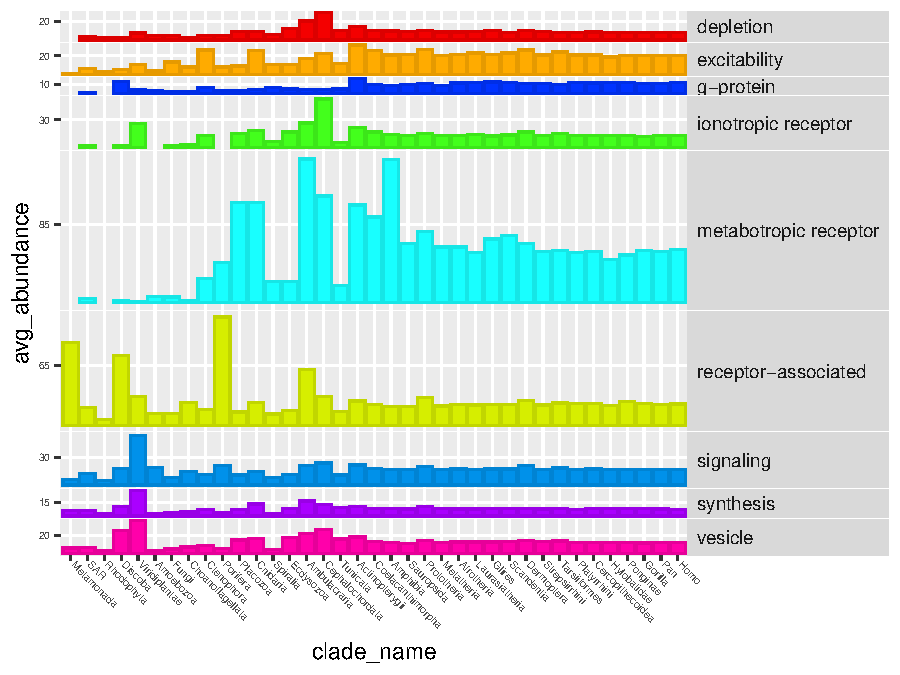
\includegraphics{figs/analysis.abundance.unnamed-chunk-6-1} 

}

\caption{Abundances averaged by clades.}\label{fig:unnamed-chunk-6}
\end{figure}

Plain protein abundance in single orthogroups

\begin{Shaded}
\begin{Highlighting}[]
\CommentTok{# Collapsing COGs with multiple functions}
\NormalTok{cog_abundance_collapsed <-}\StringTok{ }\NormalTok{cog_abundance_by_taxid }\OperatorTok
\StringTok{  }\KeywordTok{group_by}\NormalTok{(taxid, cog_id) }\OperatorTok
\StringTok{  }\KeywordTok{summarise}\NormalTok{(}
     \DataTypeTok{annotation =} \KeywordTok{paste}\NormalTok{(annotation, }\DataTypeTok{collapse =} \StringTok{"/"}\NormalTok{)}
\NormalTok{    ,}\DataTypeTok{abundance  =} \KeywordTok{unique}\NormalTok{(abundance)}
\NormalTok{  ) }\OperatorTok
\StringTok{  }\NormalTok{ungroup }\OperatorTok
\StringTok{  }\KeywordTok{left_join}\NormalTok{(ordered_species) }\OperatorTok
\StringTok{  }\KeywordTok{arrange}\NormalTok{(annotation) }\OperatorTok
\StringTok{  }\KeywordTok{mutate}\NormalTok{(}\DataTypeTok{cog_id =} \KeywordTok{fct_inorder}\NormalTok{(cog_id))}

\CommentTok{# Adding colors for such COGs}
\NormalTok{annotation_colors }\OperatorTok\StringTok{ }\KeywordTok{c}\NormalTok{(}
   \StringTok{"vesicle/synthesis"}\NormalTok{      =}\StringTok{ "#808080"}
\NormalTok{  ,}\StringTok{"depletion/vesicle"}\NormalTok{      =}\StringTok{ "#808080"}
\NormalTok{  ,}\StringTok{"signaling/excitability"}\NormalTok{ =}\StringTok{ "#808080"}
\NormalTok{)}

\KeywordTok{ggplot}\NormalTok{(cog_abundance_collapsed) }\OperatorTok{+}
\StringTok{  }\NormalTok{metazoa_line }\OperatorTok{+}\StringTok{ }
\StringTok{  }\KeywordTok{geom_bar}\NormalTok{(}\KeywordTok{aes}\NormalTok{(}\DataTypeTok{x =}\NormalTok{ ncbi_name, }\DataTypeTok{y =}\NormalTok{ abundance, }\DataTypeTok{fill =}\NormalTok{ annotation), }\DataTypeTok{stat =} \StringTok{"identity"}\NormalTok{) }\OperatorTok{+}
\StringTok{  }\KeywordTok{scale_fill_manual}\NormalTok{(}\DataTypeTok{values =}\NormalTok{ annotation_colors }\OperatorTok\StringTok{ }\KeywordTok{darken}\NormalTok{(}\FloatTok{0.2}\NormalTok{), }\DataTypeTok{guide =} \StringTok{"none"}\NormalTok{) }\OperatorTok{+}
\StringTok{  }\KeywordTok{scale_y_continuous}\NormalTok{(}\DataTypeTok{breaks =}\NormalTok{ tick_function, }\DataTypeTok{minor_breaks =} \OtherTok{NULL}\NormalTok{) }\OperatorTok{+}
\StringTok{  }\KeywordTok{facet_grid}\NormalTok{(cog_id }\OperatorTok{~}\StringTok{ }\NormalTok{., }\DataTypeTok{scales =} \StringTok{"free_y"}\NormalTok{) }\OperatorTok{+}
\StringTok{  }\KeywordTok{theme}\NormalTok{(}
     \DataTypeTok{panel.spacing      =} \KeywordTok{unit}\NormalTok{(}\FloatTok{0.5}\NormalTok{, }\StringTok{"pt"}\NormalTok{)}
\NormalTok{    ,}\DataTypeTok{panel.grid.major.x =} \KeywordTok{element_blank}\NormalTok{()}
\NormalTok{    ,}\DataTypeTok{panel.grid.major.y =} \KeywordTok{element_line}\NormalTok{(}\DataTypeTok{size =} \FloatTok{0.1}\NormalTok{, }\DataTypeTok{linetype =} \StringTok{"dashed"}\NormalTok{)}
\NormalTok{    ,}\DataTypeTok{strip.text.y       =} \KeywordTok{element_text}\NormalTok{(}\DataTypeTok{size =} \DecValTok{4}\NormalTok{, }\DataTypeTok{angle =} \DecValTok{0}\NormalTok{, }\DataTypeTok{hjust =} \DecValTok{0}\NormalTok{)}
\NormalTok{    ,}\DataTypeTok{axis.text.x        =} \KeywordTok{element_text}\NormalTok{(}\DataTypeTok{size =} \FloatTok{1.25}\NormalTok{, }\DataTypeTok{angle =} \DecValTok{-45}\NormalTok{, }\DataTypeTok{vjust =} \DecValTok{0}\NormalTok{, }\DataTypeTok{hjust =} \DecValTok{0}\NormalTok{)}
\NormalTok{    ,}\DataTypeTok{axis.text.y        =} \KeywordTok{element_text}\NormalTok{(}\DataTypeTok{size =} \DecValTok{4}\NormalTok{)}
\NormalTok{    ,}\DataTypeTok{axis.ticks         =} \KeywordTok{element_line}\NormalTok{(}\DataTypeTok{size =} \FloatTok{0.1}\NormalTok{)}
\NormalTok{  )}
\end{Highlighting}
\end{Shaded}

\begin{figure}

{\centering 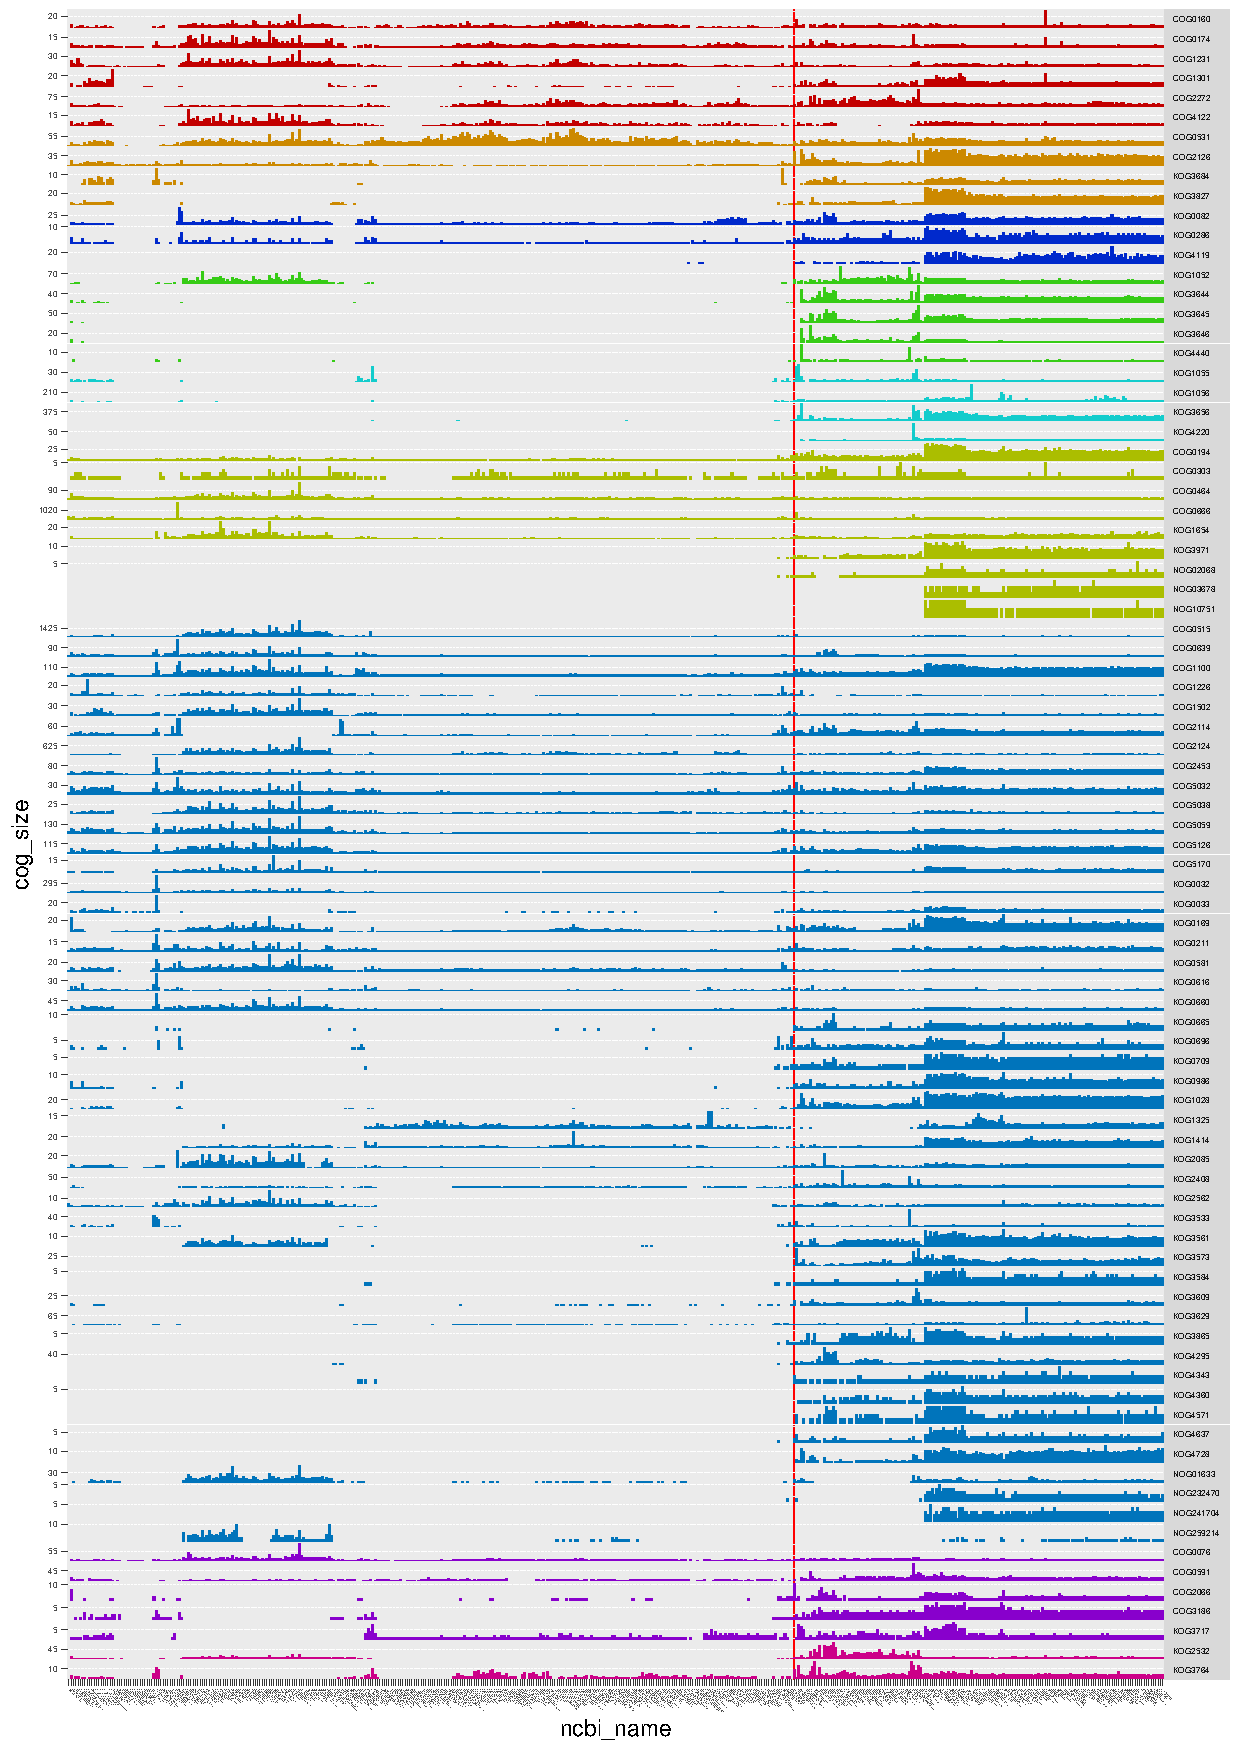
\includegraphics{figs/analysis.abundance.unnamed-chunk-7-1} 

}

\caption{Number of proteins in each neurotransmission COG, for every species.}\label{fig:unnamed-chunk-7}
\end{figure}


\begin{Shaded}
\begin{Highlighting}[]
\CommentTok{#leave this chunk}
\end{Highlighting}
\end{Shaded}

\end{document}
